\documentclass[twoside]{book}

% Packages required by doxygen
\usepackage{fixltx2e}
\usepackage{calc}
\usepackage{doxygen}
\usepackage[export]{adjustbox} % also loads graphicx
\usepackage{graphicx}
\usepackage[utf8]{inputenc}
\usepackage{makeidx}
\usepackage{multicol}
\usepackage{multirow}
\PassOptionsToPackage{warn}{textcomp}
\usepackage{textcomp}
\usepackage[nointegrals]{wasysym}
\usepackage[table]{xcolor}

% NLS support packages
\usepackage{polski}
\usepackage[T1]{fontenc}

% Font selection
\usepackage[T1]{fontenc}
\usepackage[scaled=.90]{helvet}
\usepackage{courier}
\usepackage{amssymb}
\usepackage{sectsty}
\renewcommand{\familydefault}{\sfdefault}
\allsectionsfont{%
  \fontseries{bc}\selectfont%
  \color{darkgray}%
}
\renewcommand{\DoxyLabelFont}{%
  \fontseries{bc}\selectfont%
  \color{darkgray}%
}
\newcommand{\+}{\discretionary{\mbox{\scriptsize$\hookleftarrow$}}{}{}}

% Page & text layout
\usepackage{geometry}
\geometry{%
  a4paper,%
  top=2.5cm,%
  bottom=2.5cm,%
  left=2.5cm,%
  right=2.5cm%
}
\tolerance=750
\hfuzz=15pt
\hbadness=750
\setlength{\emergencystretch}{15pt}
\setlength{\parindent}{0cm}
\setlength{\parskip}{0.2cm}
\makeatletter
\renewcommand{\paragraph}{%
  \@startsection{paragraph}{4}{0ex}{-1.0ex}{1.0ex}{%
    \normalfont\normalsize\bfseries\SS@parafont%
  }%
}
\renewcommand{\subparagraph}{%
  \@startsection{subparagraph}{5}{0ex}{-1.0ex}{1.0ex}{%
    \normalfont\normalsize\bfseries\SS@subparafont%
  }%
}
\makeatother

% Headers & footers
\usepackage{fancyhdr}
\pagestyle{fancyplain}
\fancyhead[LE]{\fancyplain{}{\bfseries\thepage}}
\fancyhead[CE]{\fancyplain{}{}}
\fancyhead[RE]{\fancyplain{}{\bfseries\leftmark}}
\fancyhead[LO]{\fancyplain{}{\bfseries\rightmark}}
\fancyhead[CO]{\fancyplain{}{}}
\fancyhead[RO]{\fancyplain{}{\bfseries\thepage}}
\fancyfoot[LE]{\fancyplain{}{}}
\fancyfoot[CE]{\fancyplain{}{}}
\fancyfoot[RE]{\fancyplain{}{\bfseries\scriptsize Wygenerowano Pn, 11 sty 2016 14\+:21\+:34 dla Game programem Doxygen }}
\fancyfoot[LO]{\fancyplain{}{\bfseries\scriptsize Wygenerowano Pn, 11 sty 2016 14\+:21\+:34 dla Game programem Doxygen }}
\fancyfoot[CO]{\fancyplain{}{}}
\fancyfoot[RO]{\fancyplain{}{}}
\renewcommand{\footrulewidth}{0.4pt}
\renewcommand{\chaptermark}[1]{%
  \markboth{#1}{}%
}
\renewcommand{\sectionmark}[1]{%
  \markright{\thesection\ #1}%
}

% Indices & bibliography
\usepackage{natbib}
\usepackage[titles]{tocloft}
\setcounter{tocdepth}{3}
\setcounter{secnumdepth}{5}
\makeindex

% Custom commands
\newcommand{\clearemptydoublepage}{%
  \newpage{\pagestyle{empty}\cleardoublepage}%
}


%===== C O N T E N T S =====

\begin{document}

% Titlepage & ToC
\pagenumbering{roman}
\begin{titlepage}
\vspace*{7cm}
\begin{center}%
{\Large Game }\\
\vspace*{1cm}
{\large Wygenerowano przez Doxygen 1.8.10}\\
\vspace*{0.5cm}
{\small Pn, 11 sty 2016 14:21:34}\\
\end{center}
\end{titlepage}
\clearemptydoublepage
\tableofcontents
\clearemptydoublepage
\pagenumbering{arabic}

%--- Begin generated contents ---
\chapter{Indeks hierarchiczny}
\section{Hierarchia klas}
Ta lista dziedziczenia posortowana jest z grubsza, choć nie całkowicie, alfabetycznie\+:\begin{DoxyCompactList}
\item \contentsline{section}{Controller\+Parameters2\+D}{\pageref{class_controller_parameters2_d}}{}
\item \contentsline{section}{Controller\+State2\+D}{\pageref{class_controller_state2_d}}{}
\item \contentsline{section}{Game\+Manager}{\pageref{class_game_manager}}{}
\item \contentsline{section}{I\+Floating\+Text\+Positioner}{\pageref{interface_i_floating_text_positioner}}{}
\begin{DoxyCompactList}
\item \contentsline{section}{Centered\+Text\+Positioner}{\pageref{class_centered_text_positioner}}{}
\item \contentsline{section}{From\+World\+Point\+Text\+Positioner}{\pageref{class_from_world_point_text_positioner}}{}
\end{DoxyCompactList}
\item \contentsline{section}{I\+Player\+Respawn\+Listener}{\pageref{interface_i_player_respawn_listener}}{}
\begin{DoxyCompactList}
\item \contentsline{section}{Give\+Health}{\pageref{class_give_health}}{}
\item \contentsline{section}{Point\+Star}{\pageref{class_point_star}}{}
\item \contentsline{section}{Simple\+Enemy\+Ai}{\pageref{class_simple_enemy_ai}}{}
\end{DoxyCompactList}
\item \contentsline{section}{I\+Take\+Damage}{\pageref{interface_i_take_damage}}{}
\begin{DoxyCompactList}
\item \contentsline{section}{Pathed\+Projectile}{\pageref{class_pathed_projectile}}{}
\item \contentsline{section}{Player}{\pageref{class_player}}{}
\item \contentsline{section}{Simple\+Enemy\+Ai}{\pageref{class_simple_enemy_ai}}{}
\end{DoxyCompactList}
\item Mono\+Behaviour\begin{DoxyCompactList}
\item \contentsline{section}{Auto\+Destroy\+Particle\+System}{\pageref{class_auto_destroy_particle_system}}{}
\item \contentsline{section}{Background\+Parallax}{\pageref{class_background_parallax}}{}
\item \contentsline{section}{Camera\+Controller}{\pageref{class_camera_controller}}{}
\item \contentsline{section}{Character\+Controller2\+D}{\pageref{class_character_controller2_d}}{}
\item \contentsline{section}{Checkpoint}{\pageref{class_checkpoint}}{}
\item \contentsline{section}{Controller\+Physics\+Volume2\+D}{\pageref{class_controller_physics_volume2_d}}{}
\item \contentsline{section}{Finish\+Level}{\pageref{class_finish_level}}{}
\item \contentsline{section}{Floating\+Text}{\pageref{class_floating_text}}{}
\item \contentsline{section}{Follow\+Object}{\pageref{class_follow_object}}{}
\item \contentsline{section}{Follow\+Path}{\pageref{class_follow_path}}{}
\item \contentsline{section}{Game\+Hud}{\pageref{class_game_hud}}{}
\item \contentsline{section}{Give\+Damage\+To\+Player}{\pageref{class_give_damage_to_player}}{}
\item \contentsline{section}{Give\+Health}{\pageref{class_give_health}}{}
\item \contentsline{section}{Health\+Bar}{\pageref{class_health_bar}}{}
\item \contentsline{section}{Insta\+Kill}{\pageref{class_insta_kill}}{}
\item \contentsline{section}{Jump\+Platform}{\pageref{class_jump_platform}}{}
\item \contentsline{section}{Level\+Manager}{\pageref{class_level_manager}}{}
\item \contentsline{section}{Path\+Definition}{\pageref{class_path_definition}}{}
\item \contentsline{section}{Pathed\+Projectile}{\pageref{class_pathed_projectile}}{}
\item \contentsline{section}{Pathed\+Projectile\+Spawner}{\pageref{class_pathed_projectile_spawner}}{}
\item \contentsline{section}{Player}{\pageref{class_player}}{}
\item \contentsline{section}{Player\+Bounds}{\pageref{class_player_bounds}}{}
\item \contentsline{section}{Point\+Star}{\pageref{class_point_star}}{}
\item \contentsline{section}{Projectile}{\pageref{class_projectile}}{}
\begin{DoxyCompactList}
\item \contentsline{section}{Simple\+Projectile}{\pageref{class_simple_projectile}}{}
\end{DoxyCompactList}
\item \contentsline{section}{Simple\+Enemy\+Ai}{\pageref{class_simple_enemy_ai}}{}
\item \contentsline{section}{Sort\+Particle\+System}{\pageref{class_sort_particle_system}}{}
\item \contentsline{section}{Start\+Screen}{\pageref{class_start_screen}}{}
\end{DoxyCompactList}
\end{DoxyCompactList}

\chapter{Indeks klas}
\section{Lista klas}
Tutaj znajdują się klasy, struktury, unie i interfejsy wraz z ich krótkimi opisami\+:\begin{DoxyCompactList}
\item\contentsline{section}{{\bf Auto\+Destroy\+Particle\+System} \\*Klasa automatycznie niszcząca particle system po zakończeniu jego animacji. }{\pageref{class_auto_destroy_particle_system}}{}
\item\contentsline{section}{{\bf Background\+Parallax} \\*klasa \doxyref{Background\+Parallax}{str.}{class_background_parallax} }{\pageref{class_background_parallax}}{}
\item\contentsline{section}{{\bf Camera\+Controller} \\*klasa \doxyref{Camera\+Controller}{str.}{class_camera_controller} }{\pageref{class_camera_controller}}{}
\item\contentsline{section}{{\bf Centered\+Text\+Positioner} \\*Klasa obsługująca wyświetlanie tekstu na środku ekranu (po wejściu w nowy checkpoint). }{\pageref{class_centered_text_positioner}}{}
\item\contentsline{section}{{\bf Character\+Controller2\+D} \\*klasa \doxyref{Character\+Controller2\+D}{str.}{class_character_controller2_d} }{\pageref{class_character_controller2_d}}{}
\item\contentsline{section}{{\bf Checkpoint} \\*Klasa odpowiedzialna za respawn gracza w danym checkpoincie. }{\pageref{class_checkpoint}}{}
\item\contentsline{section}{{\bf Controller\+Parameters2\+D} \\*klasa \doxyref{Controller\+Parameters2\+D}{str.}{class_controller_parameters2_d} }{\pageref{class_controller_parameters2_d}}{}
\item\contentsline{section}{{\bf Controller\+Physics\+Volume2\+D} \\*klasa \doxyref{Controller\+Physics\+Volume2\+D}{str.}{class_controller_physics_volume2_d} }{\pageref{class_controller_physics_volume2_d}}{}
\item\contentsline{section}{{\bf Controller\+State2\+D} \\*klasa \doxyref{Controller\+State2\+D}{str.}{class_controller_state2_d} }{\pageref{class_controller_state2_d}}{}
\item\contentsline{section}{{\bf Finish\+Level} \\*Klasa odpowiedzialna za przejście do następnego poziomu, po wejściu w obszar zmiany poziomu. }{\pageref{class_finish_level}}{}
\item\contentsline{section}{{\bf Floating\+Text} \\*Klasa odpowiedzialna za wyświetlanie na ekranie gry tekstu informującego o różnych zdarzeniach występujących w czasie rozgrywki. }{\pageref{class_floating_text}}{}
\item\contentsline{section}{{\bf Follow\+Object} \\*Klasa zapewnia podążanie pasku za graczem (w odpowiedniej odległości). }{\pageref{class_follow_object}}{}
\item\contentsline{section}{{\bf Follow\+Path} \\*klasa \doxyref{Follow\+Path}{str.}{class_follow_path} }{\pageref{class_follow_path}}{}
\item\contentsline{section}{{\bf From\+World\+Point\+Text\+Positioner} \\*Klasa określająca parametry wyświetlanego tekstu w świecie gry. }{\pageref{class_from_world_point_text_positioner}}{}
\item\contentsline{section}{{\bf Game\+Hud} \\*Klasa odpowiedzialna za wyświetlanie komunikatu o zdobytych punktach za zebranie gwiazdek i dojście do nowego checkpointu (bonus czasowy). }{\pageref{class_game_hud}}{}
\item\contentsline{section}{{\bf Game\+Manager} \\*Klasa odpowiedzialna za naliczanie i resetowanie punktów podczas gry. }{\pageref{class_game_manager}}{}
\item\contentsline{section}{{\bf Give\+Damage\+To\+Player} \\*Klasa odpowiedzialna za zadawanie obrażeń graczowi przez dany obiekt. }{\pageref{class_give_damage_to_player}}{}
\item\contentsline{section}{{\bf Give\+Health} \\*Klasa odpowiadająca za dodanie punktów zdrowia gracza po zebraniu apteczki. }{\pageref{class_give_health}}{}
\item\contentsline{section}{{\bf Health\+Bar} \\*Klasa pasku zdrowia pojawiającego się nad graczem. }{\pageref{class_health_bar}}{}
\item\contentsline{section}{{\bf I\+Floating\+Text\+Positioner} \\*Interfejs z metodą pozwalającą pobrać położenie tekstu wyświetlanego na ekranie. }{\pageref{interface_i_floating_text_positioner}}{}
\item\contentsline{section}{{\bf Insta\+Kill} \\*Klasa odpowiedzialna za zabicie gracza, gdy napotka na Collider2\+D danego obiektu. }{\pageref{class_insta_kill}}{}
\item\contentsline{section}{{\bf I\+Player\+Respawn\+Listener} \\*Interfejs odpowiedzialny za zrespawnowanie gracza w danym checkpoincie. }{\pageref{interface_i_player_respawn_listener}}{}
\item\contentsline{section}{{\bf I\+Take\+Damage} \\*Interfejs posiadający funkcją przyjmowania obrażeń o podanej wartości, zadanych przez dany obiekt. }{\pageref{interface_i_take_damage}}{}
\item\contentsline{section}{{\bf Jump\+Platform} \\*klasa \doxyref{Jump\+Platform}{str.}{class_jump_platform} }{\pageref{class_jump_platform}}{}
\item\contentsline{section}{{\bf Level\+Manager} }{\pageref{class_level_manager}}{}
\item\contentsline{section}{{\bf Path\+Definition} \\*klasa \doxyref{Path\+Definition}{str.}{class_path_definition} }{\pageref{class_path_definition}}{}
\item\contentsline{section}{{\bf Pathed\+Projectile} }{\pageref{class_pathed_projectile}}{}
\item\contentsline{section}{{\bf Pathed\+Projectile\+Spawner} \\*Tworzenie pocisku poruszającego się po danej ścieżce. }{\pageref{class_pathed_projectile_spawner}}{}
\item\contentsline{section}{{\bf Player} \\*klasa \doxyref{Player}{str.}{class_player} }{\pageref{class_player}}{}
\item\contentsline{section}{{\bf Player\+Bounds} \\*Klasa ograniczająca mozliwy ruch gracza jedynie w zakresie widzialnego istniejącego poziomu. }{\pageref{class_player_bounds}}{}
\item\contentsline{section}{{\bf Point\+Star} \\*Klasa przyznająca punkty za zebranie gwiazdek. }{\pageref{class_point_star}}{}
\item\contentsline{section}{{\bf Projectile} \\*Podstawowa klasa pocisku. }{\pageref{class_projectile}}{}
\item\contentsline{section}{{\bf Simple\+Enemy\+Ai} \\*Klasa odpowiadająca za podstawowe działania przeciwnika w świecie gry. }{\pageref{class_simple_enemy_ai}}{}
\item\contentsline{section}{{\bf Simple\+Projectile} \\*Klasa potomna dziedzicząca z \doxyref{Projectile}{str.}{class_projectile}. }{\pageref{class_simple_projectile}}{}
\item\contentsline{section}{{\bf Sort\+Particle\+System} \\*klasa \doxyref{Sort\+Particle\+System}{str.}{class_sort_particle_system} }{\pageref{class_sort_particle_system}}{}
\item\contentsline{section}{{\bf Start\+Screen} \\*Klasa umożliwi ewentualne rozpoczęcie gry od ekranu startowego, a nastepnie przeniesienie do pierwszego etapu gry. }{\pageref{class_start_screen}}{}
\end{DoxyCompactList}

\chapter{Dokumentacja klas}
\section{Dokumentacja klasy Auto\+Destroy\+Particle\+System}
\label{class_auto_destroy_particle_system}\index{Auto\+Destroy\+Particle\+System@{Auto\+Destroy\+Particle\+System}}


Klasa automatycznie niszcząca particle system po zakończeniu jego animacji.  


Diagram dziedziczenia dla Auto\+Destroy\+Particle\+System\begin{figure}[H]
\begin{center}
\leavevmode
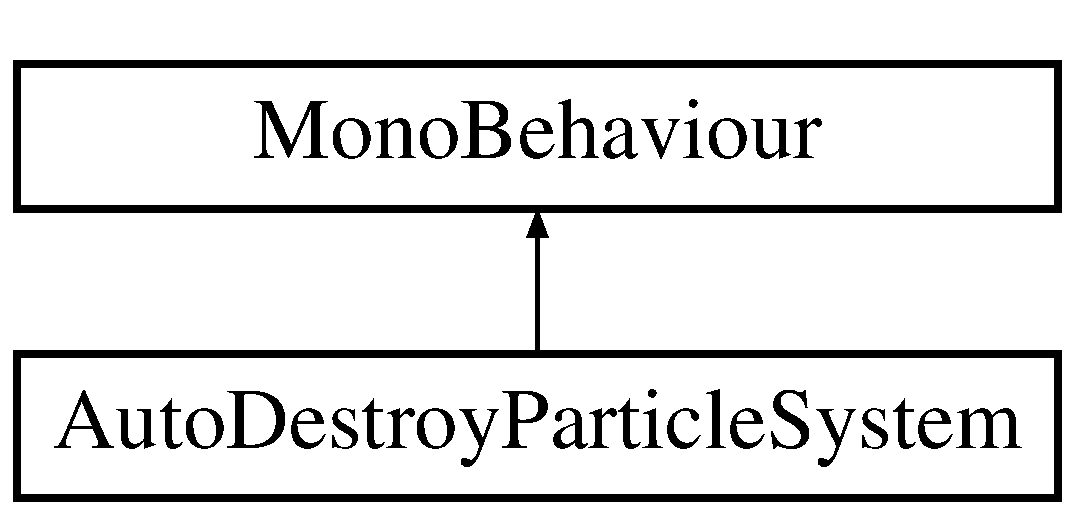
\includegraphics[height=2.000000cm]{class_auto_destroy_particle_system}
\end{center}
\end{figure}
\subsection*{Metody publiczne}
\begin{DoxyCompactItemize}
\item 
void {\bf Start} ()
\begin{DoxyCompactList}\small\item\em Pobranie Particle\+System. \end{DoxyCompactList}\item 
void {\bf Update} ()
\begin{DoxyCompactList}\small\item\em Automatyczne zniszczenie particle system po zakończeniu jego animacji. \end{DoxyCompactList}\end{DoxyCompactItemize}


\subsection{Opis szczegółowy}
Klasa automatycznie niszcząca particle system po zakończeniu jego animacji. 



\subsection{Dokumentacja funkcji składowych}
\index{Auto\+Destroy\+Particle\+System@{Auto\+Destroy\+Particle\+System}!Start@{Start}}
\index{Start@{Start}!Auto\+Destroy\+Particle\+System@{Auto\+Destroy\+Particle\+System}}
\subsubsection[{Start()}]{\setlength{\rightskip}{0pt plus 5cm}void Auto\+Destroy\+Particle\+System.\+Start (
\begin{DoxyParamCaption}
{}
\end{DoxyParamCaption}
)}\label{class_auto_destroy_particle_system_a74462c1cf75609ccd2d2663f996d2095}


Pobranie Particle\+System. 

\index{Auto\+Destroy\+Particle\+System@{Auto\+Destroy\+Particle\+System}!Update@{Update}}
\index{Update@{Update}!Auto\+Destroy\+Particle\+System@{Auto\+Destroy\+Particle\+System}}
\subsubsection[{Update()}]{\setlength{\rightskip}{0pt plus 5cm}void Auto\+Destroy\+Particle\+System.\+Update (
\begin{DoxyParamCaption}
{}
\end{DoxyParamCaption}
)}\label{class_auto_destroy_particle_system_a17e7ff9cc79dcb7b2bc8a537f0c3b042}


Automatyczne zniszczenie particle system po zakończeniu jego animacji. 



Dokumentacja dla tej klasy została wygenerowana z pliku\+:\begin{DoxyCompactItemize}
\item 
C\+:/\+Users/\+Paul/\+Projects/\+Unity\+Game/\+Projekt/\+Assets/\+Code/Auto\+Destroy\+Particle\+System.\+cs\end{DoxyCompactItemize}

\section{Dokumentacja klasy Background\+Parallax}
\label{class_background_parallax}\index{Background\+Parallax@{Background\+Parallax}}


klasa \doxyref{Background\+Parallax}{str.}{class_background_parallax}  


Diagram dziedziczenia dla Background\+Parallax\begin{figure}[H]
\begin{center}
\leavevmode
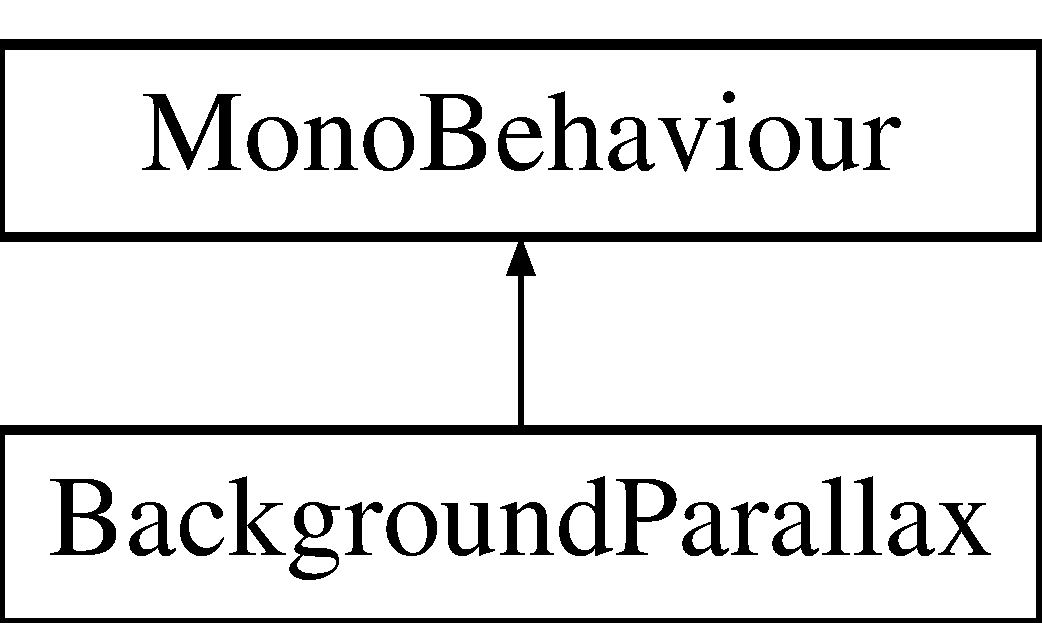
\includegraphics[height=2.000000cm]{class_background_parallax}
\end{center}
\end{figure}
\subsection*{Metody publiczne}
\begin{DoxyCompactItemize}
\item 
void {\bf start} ()
\begin{DoxyCompactList}\small\item\em Zapamiętanie położenia kamery w ostatniej klatce gry, potrzebnego w późniejszym etape do określenia, o ile tło musi się poruszyć w lewo lub prawo. \end{DoxyCompactList}\item 
void {\bf Update} ()
\begin{DoxyCompactList}\small\item\em Ruch wykonany od ostaniej klatki do obecnej, przeskalowany przez czynnik efektu parallax (intensywności ruchu tła). \end{DoxyCompactList}\end{DoxyCompactItemize}
\subsection*{Atrybuty publiczne}
\begin{DoxyCompactItemize}
\item 
Transform[$\,$] {\bf Backgrounds}
\begin{DoxyCompactList}\small\item\em Tablica rzędów elementów tła. \end{DoxyCompactList}\item 
float {\bf Parallax\+Scale}
\begin{DoxyCompactList}\small\item\em Wartość efektu poruszania się tła. \end{DoxyCompactList}\item 
float {\bf Parallax\+Reduction\+Factor}
\begin{DoxyCompactList}\small\item\em Wartość redukująca stopień poruszania się, dla warstw (rzędów elementów) dalej położonych. \end{DoxyCompactList}\item 
float {\bf Smoothing}
\begin{DoxyCompactList}\small\item\em Zapewnienie płynności ruchu. \end{DoxyCompactList}\end{DoxyCompactItemize}


\subsection{Opis szczegółowy}
klasa \doxyref{Background\+Parallax}{str.}{class_background_parallax} 



\subsection{Dokumentacja funkcji składowych}
\index{Background\+Parallax@{Background\+Parallax}!start@{start}}
\index{start@{start}!Background\+Parallax@{Background\+Parallax}}
\subsubsection[{start()}]{\setlength{\rightskip}{0pt plus 5cm}void Background\+Parallax.\+start (
\begin{DoxyParamCaption}
{}
\end{DoxyParamCaption}
)}\label{class_background_parallax_abb5fc2464be1a1bba55238be509a2082}


Zapamiętanie położenia kamery w ostatniej klatce gry, potrzebnego w późniejszym etape do określenia, o ile tło musi się poruszyć w lewo lub prawo. 

\index{Background\+Parallax@{Background\+Parallax}!Update@{Update}}
\index{Update@{Update}!Background\+Parallax@{Background\+Parallax}}
\subsubsection[{Update()}]{\setlength{\rightskip}{0pt plus 5cm}void Background\+Parallax.\+Update (
\begin{DoxyParamCaption}
{}
\end{DoxyParamCaption}
)}\label{class_background_parallax_a77b333e27f605355ee6b98eb58641ab5}


Ruch wykonany od ostaniej klatki do obecnej, przeskalowany przez czynnik efektu parallax (intensywności ruchu tła). 

Dla każdej warstwy (rzędu elementów) tła.

Zapamiętanie pozycji warstwy tła uaktualnionej o efekt parallax,

oraz postepującą redukcję tego efektu dla coraz dalszych warstw.

Ustawienie aktualnej pozycji warstw tła.

Obecna pozycja tła.

Nowa pozycja tła.

Określony efekt płynności animacji efektu w grze.

Uaktualnienie ruchu kamery. 

\subsection{Dokumentacja atrybutów składowych}
\index{Background\+Parallax@{Background\+Parallax}!Backgrounds@{Backgrounds}}
\index{Backgrounds@{Backgrounds}!Background\+Parallax@{Background\+Parallax}}
\subsubsection[{Backgrounds}]{\setlength{\rightskip}{0pt plus 5cm}Transform [$\,$] Background\+Parallax.\+Backgrounds}\label{class_background_parallax_a626641e92b9bedfbd0f5aaf2938875b3}


Tablica rzędów elementów tła. 

\index{Background\+Parallax@{Background\+Parallax}!Parallax\+Reduction\+Factor@{Parallax\+Reduction\+Factor}}
\index{Parallax\+Reduction\+Factor@{Parallax\+Reduction\+Factor}!Background\+Parallax@{Background\+Parallax}}
\subsubsection[{Parallax\+Reduction\+Factor}]{\setlength{\rightskip}{0pt plus 5cm}float Background\+Parallax.\+Parallax\+Reduction\+Factor}\label{class_background_parallax_aad6f6a27f24a5d911991227f8abe1a71}


Wartość redukująca stopień poruszania się, dla warstw (rzędów elementów) dalej położonych. 

\index{Background\+Parallax@{Background\+Parallax}!Parallax\+Scale@{Parallax\+Scale}}
\index{Parallax\+Scale@{Parallax\+Scale}!Background\+Parallax@{Background\+Parallax}}
\subsubsection[{Parallax\+Scale}]{\setlength{\rightskip}{0pt plus 5cm}float Background\+Parallax.\+Parallax\+Scale}\label{class_background_parallax_a078a366dfc612de0f0848b9be330f055}


Wartość efektu poruszania się tła. 

\index{Background\+Parallax@{Background\+Parallax}!Smoothing@{Smoothing}}
\index{Smoothing@{Smoothing}!Background\+Parallax@{Background\+Parallax}}
\subsubsection[{Smoothing}]{\setlength{\rightskip}{0pt plus 5cm}float Background\+Parallax.\+Smoothing}\label{class_background_parallax_ad9e09d728695d0c26f103ee614b67000}


Zapewnienie płynności ruchu. 



Dokumentacja dla tej klasy została wygenerowana z pliku\+:\begin{DoxyCompactItemize}
\item 
C\+:/\+Users/\+Paul/\+Projects/\+Unity\+Game/\+Projekt/\+Assets/\+Code/Background\+Parallax.\+cs\end{DoxyCompactItemize}

\section{Dokumentacja klasy Camera\+Controller}
\label{class_camera_controller}\index{Camera\+Controller@{Camera\+Controller}}


klasa \doxyref{Camera\+Controller}{str.}{class_camera_controller}  


Diagram dziedziczenia dla Camera\+Controller\begin{figure}[H]
\begin{center}
\leavevmode
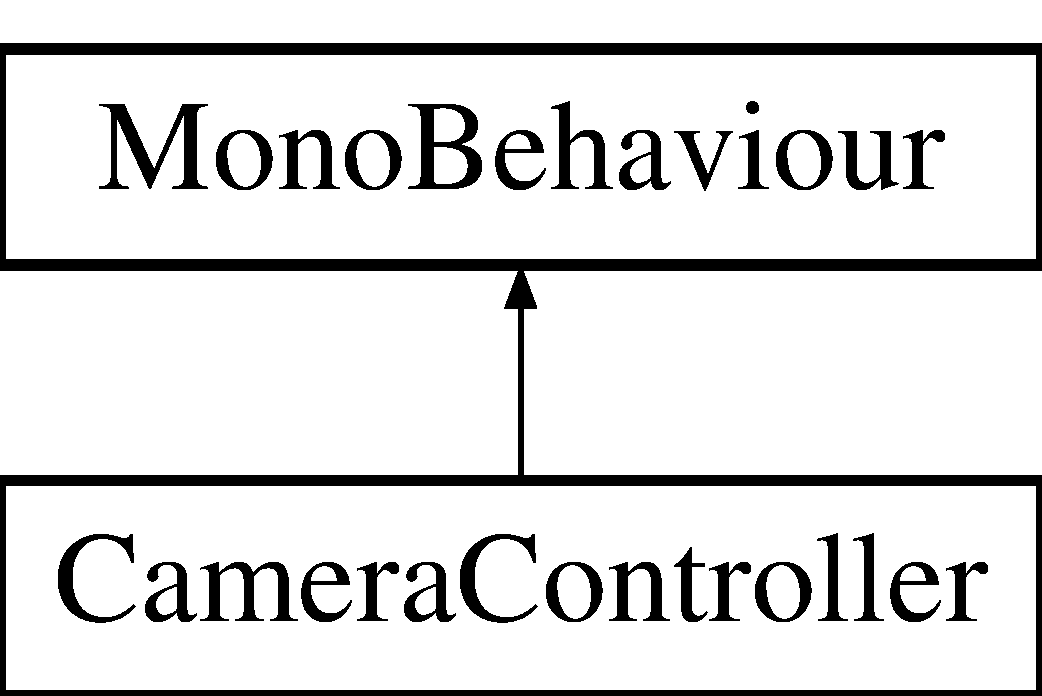
\includegraphics[height=2.000000cm]{class_camera_controller}
\end{center}
\end{figure}
\subsection*{Metody publiczne}
\begin{DoxyCompactItemize}
\item 
void {\bf Start} ()
\begin{DoxyCompactList}\small\item\em Ustawienie ograniczeń rozmiaru obszaru, w którym może się poruszać kamera, oraz ustawienie podążania kamery za graczem. \end{DoxyCompactList}\item 
void {\bf Update} ()
\begin{DoxyCompactList}\small\item\em Metoda Update \end{DoxyCompactList}\end{DoxyCompactItemize}
\subsection*{Atrybuty publiczne}
\begin{DoxyCompactItemize}
\item 
Transform {\bf Player}
\begin{DoxyCompactList}\small\item\em Obiekt gracza. \end{DoxyCompactList}\item 
Vector2 {\bf Margin}
\begin{DoxyCompactList}\small\item\em Wartość progu ruchu gracza, od którego ma nastapić zmiana położenia kamery. \end{DoxyCompactList}\item 
Vector2 {\bf Smoothing}
\begin{DoxyCompactList}\small\item\em Zapewnienie płynności ruchu kamery. \end{DoxyCompactList}\item 
Box\+Collider2\+D {\bf Bounds}
\begin{DoxyCompactList}\small\item\em Ograniczenia ruchu kamery w świecie gry. \end{DoxyCompactList}\end{DoxyCompactItemize}
\subsection*{Właściwości}
\begin{DoxyCompactItemize}
\item 
bool {\bf Is\+Following}\hspace{0.3cm}{\ttfamily  [get, set]}
\begin{DoxyCompactList}\small\item\em Zmienna, mówiąca, czy kamera podąża za graczem. \end{DoxyCompactList}\end{DoxyCompactItemize}


\subsection{Opis szczegółowy}
klasa \doxyref{Camera\+Controller}{str.}{class_camera_controller} 



\subsection{Dokumentacja funkcji składowych}
\index{Camera\+Controller@{Camera\+Controller}!Start@{Start}}
\index{Start@{Start}!Camera\+Controller@{Camera\+Controller}}
\subsubsection[{Start()}]{\setlength{\rightskip}{0pt plus 5cm}void Camera\+Controller.\+Start (
\begin{DoxyParamCaption}
{}
\end{DoxyParamCaption}
)}\label{class_camera_controller_ad4a238c6f7db3ee003302a245d860860}


Ustawienie ograniczeń rozmiaru obszaru, w którym może się poruszać kamera, oraz ustawienie podążania kamery za graczem. 

\index{Camera\+Controller@{Camera\+Controller}!Update@{Update}}
\index{Update@{Update}!Camera\+Controller@{Camera\+Controller}}
\subsubsection[{Update()}]{\setlength{\rightskip}{0pt plus 5cm}void Camera\+Controller.\+Update (
\begin{DoxyParamCaption}
{}
\end{DoxyParamCaption}
)}\label{class_camera_controller_a7c4f486f4bcbd1d54a346fdce9707bd5}


Metoda Update 

Obecne położenie kamery.

Jeśli odległość między położeniem kamery, a położeniem gracza w poziomie jest większa od danej wartości.

Wykonaj ruch kamery z pozycji x do pozycji gracza, z określonym efektem płynności w grze.

Jeśli odległość między położeniem kamery, a położeniem gracza w pionie jest większa od danej wartości.

Wykonaj ruch kamery z pozycji y do pozycji gracza, z określonym efektem płynności w grze.

camera.\+ortographic\+Size to połowa wysokości boxu kamery. Mnożymy tę wartośc przez stosunek szerokości do wysokości, aby otrzymać połowę szerokości boxu kamery.

Ograniczanie położenia kamery (x,y) do rozmiarów Bounds, czyli boxu ograniczającego ruch kamery w świecie gry.

Ustawienie uaktualnionej pozycji kamery. 

\subsection{Dokumentacja atrybutów składowych}
\index{Camera\+Controller@{Camera\+Controller}!Bounds@{Bounds}}
\index{Bounds@{Bounds}!Camera\+Controller@{Camera\+Controller}}
\subsubsection[{Bounds}]{\setlength{\rightskip}{0pt plus 5cm}Box\+Collider2\+D Camera\+Controller.\+Bounds}\label{class_camera_controller_aad472aa9d9410f6b05884b0d4d336d45}


Ograniczenia ruchu kamery w świecie gry. 

\index{Camera\+Controller@{Camera\+Controller}!Margin@{Margin}}
\index{Margin@{Margin}!Camera\+Controller@{Camera\+Controller}}
\subsubsection[{Margin}]{\setlength{\rightskip}{0pt plus 5cm}Vector2 Camera\+Controller.\+Margin}\label{class_camera_controller_a8c93ba738eeff2eb5af4bc2bc4ec3f10}


Wartość progu ruchu gracza, od którego ma nastapić zmiana położenia kamery. 

\index{Camera\+Controller@{Camera\+Controller}!Player@{Player}}
\index{Player@{Player}!Camera\+Controller@{Camera\+Controller}}
\subsubsection[{Player}]{\setlength{\rightskip}{0pt plus 5cm}Transform Camera\+Controller.\+Player}\label{class_camera_controller_a0028f1f6c8d940c36cfb6f6ea77b8658}


Obiekt gracza. 

\index{Camera\+Controller@{Camera\+Controller}!Smoothing@{Smoothing}}
\index{Smoothing@{Smoothing}!Camera\+Controller@{Camera\+Controller}}
\subsubsection[{Smoothing}]{\setlength{\rightskip}{0pt plus 5cm}Vector2 Camera\+Controller.\+Smoothing}\label{class_camera_controller_aaa266990dfb97f6e19d4dd6489f683ef}


Zapewnienie płynności ruchu kamery. 



\subsection{Dokumentacja właściwości}
\index{Camera\+Controller@{Camera\+Controller}!Is\+Following@{Is\+Following}}
\index{Is\+Following@{Is\+Following}!Camera\+Controller@{Camera\+Controller}}
\subsubsection[{Is\+Following}]{\setlength{\rightskip}{0pt plus 5cm}bool Camera\+Controller.\+Is\+Following\hspace{0.3cm}{\ttfamily [get]}, {\ttfamily [set]}}\label{class_camera_controller_a1eb503b3ec9f5c4b2f267e859ba37467}


Zmienna, mówiąca, czy kamera podąża za graczem. 



Dokumentacja dla tej klasy została wygenerowana z pliku\+:\begin{DoxyCompactItemize}
\item 
C\+:/\+Users/\+Paul/\+Projects/\+Unity\+Game/\+Projekt/\+Assets/\+Code/Camera\+Controller.\+cs\end{DoxyCompactItemize}

\section{Dokumentacja klasy Centered\+Text\+Positioner}
\label{class_centered_text_positioner}\index{Centered\+Text\+Positioner@{Centered\+Text\+Positioner}}


Klasa obsługująca wyświetlanie tekstu na środku ekranu (po wejściu w nowy checkpoint).  


Diagram dziedziczenia dla Centered\+Text\+Positioner\begin{figure}[H]
\begin{center}
\leavevmode
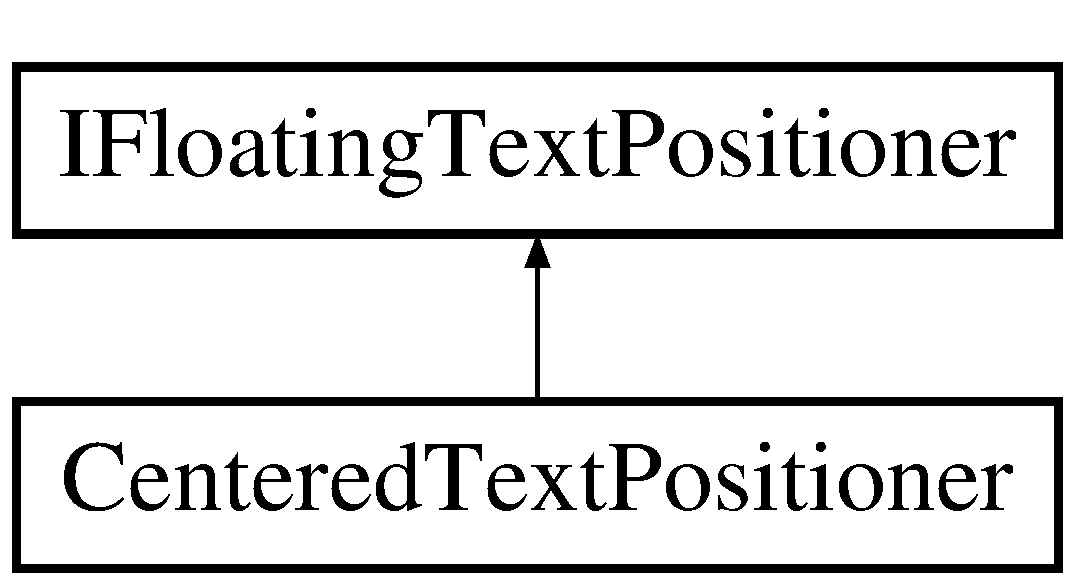
\includegraphics[height=2.000000cm]{class_centered_text_positioner}
\end{center}
\end{figure}
\subsection*{Metody publiczne}
\begin{DoxyCompactItemize}
\item 
{\bf Centered\+Text\+Positioner} (float speed)
\begin{DoxyCompactList}\small\item\em Ustawienie szybkości wyświetlania komunikatów tekstowych. \end{DoxyCompactList}\item 
bool {\bf Get\+Position} (ref Vector2 position, G\+U\+I\+Content content, Vector2 size)
\begin{DoxyCompactList}\small\item\em Metoda mówiąca \doxyref{Floating\+Text}{str.}{class_floating_text}, czy dalej wyświetlać tekst. Ustawia również współrzędne tekstu w grze. \end{DoxyCompactList}\end{DoxyCompactItemize}


\subsection{Opis szczegółowy}
Klasa obsługująca wyświetlanie tekstu na środku ekranu (po wejściu w nowy checkpoint). 



\subsection{Dokumentacja konstruktora i destruktora}
\index{Centered\+Text\+Positioner@{Centered\+Text\+Positioner}!Centered\+Text\+Positioner@{Centered\+Text\+Positioner}}
\index{Centered\+Text\+Positioner@{Centered\+Text\+Positioner}!Centered\+Text\+Positioner@{Centered\+Text\+Positioner}}
\subsubsection[{Centered\+Text\+Positioner(float speed)}]{\setlength{\rightskip}{0pt plus 5cm}Centered\+Text\+Positioner.\+Centered\+Text\+Positioner (
\begin{DoxyParamCaption}
\item[{float}]{speed}
\end{DoxyParamCaption}
)}\label{class_centered_text_positioner_a60ca0fe6eff20d40d78b69c456999163}


Ustawienie szybkości wyświetlania komunikatów tekstowych. 


\begin{DoxyParams}{Parametry}
{\em speed} & \\
\hline
\end{DoxyParams}


\subsection{Dokumentacja funkcji składowych}
\index{Centered\+Text\+Positioner@{Centered\+Text\+Positioner}!Get\+Position@{Get\+Position}}
\index{Get\+Position@{Get\+Position}!Centered\+Text\+Positioner@{Centered\+Text\+Positioner}}
\subsubsection[{Get\+Position(ref Vector2 position, G\+U\+I\+Content content, Vector2 size)}]{\setlength{\rightskip}{0pt plus 5cm}bool Centered\+Text\+Positioner.\+Get\+Position (
\begin{DoxyParamCaption}
\item[{ref Vector2}]{position, }
\item[{G\+U\+I\+Content}]{content, }
\item[{Vector2}]{size}
\end{DoxyParamCaption}
)}\label{class_centered_text_positioner_ad620db2ea6222bd334b95e0b4e50464d}


Metoda mówiąca \doxyref{Floating\+Text}{str.}{class_floating_text}, czy dalej wyświetlać tekst. Ustawia również współrzędne tekstu w grze. 


\begin{DoxyParams}{Parametry}
{\em position} & \\
\hline
{\em content} & \\
\hline
{\em size} & \\
\hline
\end{DoxyParams}
\begin{DoxyReturn}{Zwraca}

\end{DoxyReturn}
Jeśli \+\_\+text\+Position osiągnie 1, tekst nie będzie dalej wyświetlany.

Ustawienie pozycji tekstu na ekranie. 

Implementuje {\bf I\+Floating\+Text\+Positioner} \doxyref{}{str.}{interface_i_floating_text_positioner}.



Dokumentacja dla tej klasy została wygenerowana z pliku\+:\begin{DoxyCompactItemize}
\item 
C\+:/\+Users/\+Paul/\+Projects/\+Unity\+Game/\+Projekt/\+Assets/\+Code/Centered\+Text\+Positioner.\+cs\end{DoxyCompactItemize}

\section{Dokumentacja klasy Character\+Controller2\+D}
\label{class_character_controller2_d}\index{Character\+Controller2\+D@{Character\+Controller2\+D}}


klasa \doxyref{Character\+Controller2\+D}{str.}{class_character_controller2_d}  


Diagram dziedziczenia dla Character\+Controller2\+D\begin{figure}[H]
\begin{center}
\leavevmode
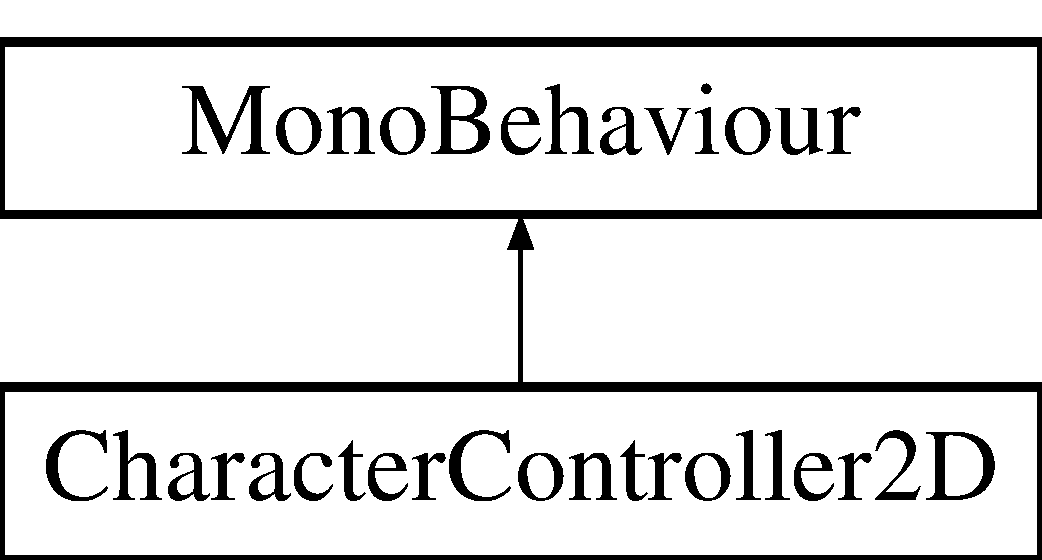
\includegraphics[height=2.000000cm]{class_character_controller2_d}
\end{center}
\end{figure}
\subsection*{Metody publiczne}
\begin{DoxyCompactItemize}
\item 
void {\bf Awake} ()
\begin{DoxyCompactList}\small\item\em Inicjalizacja i ustawienie poczatkowych wartosci parametrow. \end{DoxyCompactList}\item 
void {\bf Add\+Force} (Vector2 force)
\begin{DoxyCompactList}\small\item\em Dodanie dodatkowej predkosci. \end{DoxyCompactList}\item 
void {\bf Set\+Force} (Vector2 force)
\begin{DoxyCompactList}\small\item\em Ustawienie predkosci. \end{DoxyCompactList}\item 
void {\bf Set\+Horizontal\+Force} (float x)
\begin{DoxyCompactList}\small\item\em Ustawienie predkosci w poziomie. \end{DoxyCompactList}\item 
void {\bf Set\+Vertical\+Force} (float y)
\begin{DoxyCompactList}\small\item\em Ustawienie predkosci w pionie. \end{DoxyCompactList}\item 
void {\bf Jump} ()
\begin{DoxyCompactList}\small\item\em Wykonanie skoku. \end{DoxyCompactList}\item 
void {\bf Late\+Update} ()
\begin{DoxyCompactList}\small\item\em Wykonywane po wywolaniu aktualizacji obiektow. Uwzglednienie wplywu czasu na czestotliwosc skokow i ruch, wplyw grawitacji na ruch w pionie. \end{DoxyCompactList}\item 
void {\bf On\+Trigger\+Enter2\+D} (Collider2\+D other)
\begin{DoxyCompactList}\small\item\em Wykrycie ze gracz znalazl sie w innym srodowisku (np. wodzie). \end{DoxyCompactList}\item 
void {\bf On\+Trigger\+Exit2\+D} (Collider2\+D other)
\begin{DoxyCompactList}\small\item\em Wyjscie ze srodowiska o zmienionych parametrach. \end{DoxyCompactList}\end{DoxyCompactItemize}
\subsection*{Atrybuty publiczne}
\begin{DoxyCompactItemize}
\item 
Layer\+Mask {\bf Platform\+Mask}
\begin{DoxyCompactList}\small\item\em Layer mask uzywany do wykrywania kolizji. Obiekty na tej warstwie uczestnicza w kolizji. \end{DoxyCompactList}\item 
{\bf Controller\+Parameters2\+D} {\bf Default\+Parameters}
\begin{DoxyCompactList}\small\item\em Domyslne parametry kontrolera. \end{DoxyCompactList}\end{DoxyCompactItemize}
\subsection*{Właściwości}
\begin{DoxyCompactItemize}
\item 
{\bf Controller\+State2\+D} {\bf State}\hspace{0.3cm}{\ttfamily  [get]}
\begin{DoxyCompactList}\small\item\em Stan gracza, informujacy o kolizjach w jakich bierze udzial. \end{DoxyCompactList}\item 
Vector2 {\bf Velocity}\hspace{0.3cm}{\ttfamily  [get]}
\begin{DoxyCompactList}\small\item\em Predkosc gracza. \end{DoxyCompactList}\item 
bool {\bf Handle\+Collisions}\hspace{0.3cm}{\ttfamily  [get, set]}
\begin{DoxyCompactList}\small\item\em Zmienna typu bool, mowiaca czy nalezy obsluzyc kolizje. \end{DoxyCompactList}\item 
{\bf Controller\+Parameters2\+D} {\bf Parameters}\hspace{0.3cm}{\ttfamily  [get]}
\begin{DoxyCompactList}\small\item\em Zwraca nadpisane lub w przypadku braku nadpisania, domyslne parametry kontrolera. \end{DoxyCompactList}\item 
Game\+Object {\bf Standing\+On}\hspace{0.3cm}{\ttfamily  [get]}
\begin{DoxyCompactList}\small\item\em Standing\+On \end{DoxyCompactList}\item 
Vector3 {\bf Platform\+Velocity}\hspace{0.3cm}{\ttfamily  [get]}
\begin{DoxyCompactList}\small\item\em Predkosc platformy, na ktorej stoi gracz. \end{DoxyCompactList}\item 
bool {\bf Can\+Jump}\hspace{0.3cm}{\ttfamily  [get]}
\begin{DoxyCompactList}\small\item\em Sprawdza czy mozna wykonac skok zaleznie od ustawionej wartosci Jump\+Behavior. \end{DoxyCompactList}\end{DoxyCompactItemize}


\subsection{Opis szczegółowy}
klasa \doxyref{Character\+Controller2\+D}{str.}{class_character_controller2_d} 



\subsection{Dokumentacja funkcji składowych}
\index{Character\+Controller2\+D@{Character\+Controller2\+D}!Add\+Force@{Add\+Force}}
\index{Add\+Force@{Add\+Force}!Character\+Controller2\+D@{Character\+Controller2\+D}}
\subsubsection[{Add\+Force(\+Vector2 force)}]{\setlength{\rightskip}{0pt plus 5cm}void Character\+Controller2\+D.\+Add\+Force (
\begin{DoxyParamCaption}
\item[{Vector2}]{force}
\end{DoxyParamCaption}
)}\label{class_character_controller2_d_adbd530fe94a846d57ed2c9f322491ab3}


Dodanie dodatkowej predkosci. 

\index{Character\+Controller2\+D@{Character\+Controller2\+D}!Awake@{Awake}}
\index{Awake@{Awake}!Character\+Controller2\+D@{Character\+Controller2\+D}}
\subsubsection[{Awake()}]{\setlength{\rightskip}{0pt plus 5cm}void Character\+Controller2\+D.\+Awake (
\begin{DoxyParamCaption}
{}
\end{DoxyParamCaption}
)}\label{class_character_controller2_d_a63dec3eea904614ce11fff4d0b1f3374}


Inicjalizacja i ustawienie poczatkowych wartosci parametrow. 

Obliczenie rozmiarow boxu, ktory moze uczestniczyc w kolizjach z innymi brylami sztywnymi. Od wartosci odejmowane sa skiny, z ktorych wychodza promienie wykrywajace kolizje (skin to waska ramka wokol obiektu, istniejaca po wewnetrznej stronie obiektu, sluzaca do wykrywania kolizji). Nastepnie obliczane sa odstepy pomiedzy promieniami wykrywajacymi kolizje. \index{Character\+Controller2\+D@{Character\+Controller2\+D}!Jump@{Jump}}
\index{Jump@{Jump}!Character\+Controller2\+D@{Character\+Controller2\+D}}
\subsubsection[{Jump()}]{\setlength{\rightskip}{0pt plus 5cm}void Character\+Controller2\+D.\+Jump (
\begin{DoxyParamCaption}
{}
\end{DoxyParamCaption}
)}\label{class_character_controller2_d_aa42cc475784c2a2f5ca406669504824e}


Wykonanie skoku. 

\index{Character\+Controller2\+D@{Character\+Controller2\+D}!Late\+Update@{Late\+Update}}
\index{Late\+Update@{Late\+Update}!Character\+Controller2\+D@{Character\+Controller2\+D}}
\subsubsection[{Late\+Update()}]{\setlength{\rightskip}{0pt plus 5cm}void Character\+Controller2\+D.\+Late\+Update (
\begin{DoxyParamCaption}
{}
\end{DoxyParamCaption}
)}\label{class_character_controller2_d_aa16cb1f7b8c01f326f8b0b1508590dd7}


Wykonywane po wywolaniu aktualizacji obiektow. Uwzglednienie wplywu czasu na czestotliwosc skokow i ruch, wplyw grawitacji na ruch w pionie. 

\index{Character\+Controller2\+D@{Character\+Controller2\+D}!On\+Trigger\+Enter2\+D@{On\+Trigger\+Enter2\+D}}
\index{On\+Trigger\+Enter2\+D@{On\+Trigger\+Enter2\+D}!Character\+Controller2\+D@{Character\+Controller2\+D}}
\subsubsection[{On\+Trigger\+Enter2\+D(\+Collider2\+D other)}]{\setlength{\rightskip}{0pt plus 5cm}void Character\+Controller2\+D.\+On\+Trigger\+Enter2\+D (
\begin{DoxyParamCaption}
\item[{Collider2\+D}]{other}
\end{DoxyParamCaption}
)}\label{class_character_controller2_d_a9ac0f6a16c9a0e7190e5645a9ba77667}


Wykrycie ze gracz znalazl sie w innym srodowisku (np. wodzie). 

Nadpisanie parametrow kontrolera. \index{Character\+Controller2\+D@{Character\+Controller2\+D}!On\+Trigger\+Exit2\+D@{On\+Trigger\+Exit2\+D}}
\index{On\+Trigger\+Exit2\+D@{On\+Trigger\+Exit2\+D}!Character\+Controller2\+D@{Character\+Controller2\+D}}
\subsubsection[{On\+Trigger\+Exit2\+D(\+Collider2\+D other)}]{\setlength{\rightskip}{0pt plus 5cm}void Character\+Controller2\+D.\+On\+Trigger\+Exit2\+D (
\begin{DoxyParamCaption}
\item[{Collider2\+D}]{other}
\end{DoxyParamCaption}
)}\label{class_character_controller2_d_a91e2f7eefc4b8e8590f8eca161d9a655}


Wyjscie ze srodowiska o zmienionych parametrach. 

Parametry nie sa juz nadpisywane poprzednimi wartosciami. \index{Character\+Controller2\+D@{Character\+Controller2\+D}!Set\+Force@{Set\+Force}}
\index{Set\+Force@{Set\+Force}!Character\+Controller2\+D@{Character\+Controller2\+D}}
\subsubsection[{Set\+Force(\+Vector2 force)}]{\setlength{\rightskip}{0pt plus 5cm}void Character\+Controller2\+D.\+Set\+Force (
\begin{DoxyParamCaption}
\item[{Vector2}]{force}
\end{DoxyParamCaption}
)}\label{class_character_controller2_d_a5ed35a778ec714e5783d6f0570bca703}


Ustawienie predkosci. 

\index{Character\+Controller2\+D@{Character\+Controller2\+D}!Set\+Horizontal\+Force@{Set\+Horizontal\+Force}}
\index{Set\+Horizontal\+Force@{Set\+Horizontal\+Force}!Character\+Controller2\+D@{Character\+Controller2\+D}}
\subsubsection[{Set\+Horizontal\+Force(float x)}]{\setlength{\rightskip}{0pt plus 5cm}void Character\+Controller2\+D.\+Set\+Horizontal\+Force (
\begin{DoxyParamCaption}
\item[{float}]{x}
\end{DoxyParamCaption}
)}\label{class_character_controller2_d_a8fd797b25fef289cbc1993f94dfb9b48}


Ustawienie predkosci w poziomie. 

\index{Character\+Controller2\+D@{Character\+Controller2\+D}!Set\+Vertical\+Force@{Set\+Vertical\+Force}}
\index{Set\+Vertical\+Force@{Set\+Vertical\+Force}!Character\+Controller2\+D@{Character\+Controller2\+D}}
\subsubsection[{Set\+Vertical\+Force(float y)}]{\setlength{\rightskip}{0pt plus 5cm}void Character\+Controller2\+D.\+Set\+Vertical\+Force (
\begin{DoxyParamCaption}
\item[{float}]{y}
\end{DoxyParamCaption}
)}\label{class_character_controller2_d_a29d14b0bb79f8661d9655ab9bed074e2}


Ustawienie predkosci w pionie. 



\subsection{Dokumentacja atrybutów składowych}
\index{Character\+Controller2\+D@{Character\+Controller2\+D}!Default\+Parameters@{Default\+Parameters}}
\index{Default\+Parameters@{Default\+Parameters}!Character\+Controller2\+D@{Character\+Controller2\+D}}
\subsubsection[{Default\+Parameters}]{\setlength{\rightskip}{0pt plus 5cm}{\bf Controller\+Parameters2\+D} Character\+Controller2\+D.\+Default\+Parameters}\label{class_character_controller2_d_a33b6d08469389f16262f8a179ec3c873}


Domyslne parametry kontrolera. 

\index{Character\+Controller2\+D@{Character\+Controller2\+D}!Platform\+Mask@{Platform\+Mask}}
\index{Platform\+Mask@{Platform\+Mask}!Character\+Controller2\+D@{Character\+Controller2\+D}}
\subsubsection[{Platform\+Mask}]{\setlength{\rightskip}{0pt plus 5cm}Layer\+Mask Character\+Controller2\+D.\+Platform\+Mask}\label{class_character_controller2_d_a239fc145e05e239c584bf7b1783b590e}


Layer mask uzywany do wykrywania kolizji. Obiekty na tej warstwie uczestnicza w kolizji. 



\subsection{Dokumentacja właściwości}
\index{Character\+Controller2\+D@{Character\+Controller2\+D}!Can\+Jump@{Can\+Jump}}
\index{Can\+Jump@{Can\+Jump}!Character\+Controller2\+D@{Character\+Controller2\+D}}
\subsubsection[{Can\+Jump}]{\setlength{\rightskip}{0pt plus 5cm}bool Character\+Controller2\+D.\+Can\+Jump\hspace{0.3cm}{\ttfamily [get]}}\label{class_character_controller2_d_a79855579d0cbd33e1ed08df1c513bb0f}


Sprawdza czy mozna wykonac skok zaleznie od ustawionej wartosci Jump\+Behavior. 

\index{Character\+Controller2\+D@{Character\+Controller2\+D}!Handle\+Collisions@{Handle\+Collisions}}
\index{Handle\+Collisions@{Handle\+Collisions}!Character\+Controller2\+D@{Character\+Controller2\+D}}
\subsubsection[{Handle\+Collisions}]{\setlength{\rightskip}{0pt plus 5cm}bool Character\+Controller2\+D.\+Handle\+Collisions\hspace{0.3cm}{\ttfamily [get]}, {\ttfamily [set]}}\label{class_character_controller2_d_aa693a23e691347cf526060141fad519e}


Zmienna typu bool, mowiaca czy nalezy obsluzyc kolizje. 

\index{Character\+Controller2\+D@{Character\+Controller2\+D}!Parameters@{Parameters}}
\index{Parameters@{Parameters}!Character\+Controller2\+D@{Character\+Controller2\+D}}
\subsubsection[{Parameters}]{\setlength{\rightskip}{0pt plus 5cm}{\bf Controller\+Parameters2\+D} Character\+Controller2\+D.\+Parameters\hspace{0.3cm}{\ttfamily [get]}}\label{class_character_controller2_d_a408542bab9592c3d0d4ca432a5775ce6}


Zwraca nadpisane lub w przypadku braku nadpisania, domyslne parametry kontrolera. 

\index{Character\+Controller2\+D@{Character\+Controller2\+D}!Platform\+Velocity@{Platform\+Velocity}}
\index{Platform\+Velocity@{Platform\+Velocity}!Character\+Controller2\+D@{Character\+Controller2\+D}}
\subsubsection[{Platform\+Velocity}]{\setlength{\rightskip}{0pt plus 5cm}Vector3 Character\+Controller2\+D.\+Platform\+Velocity\hspace{0.3cm}{\ttfamily [get]}}\label{class_character_controller2_d_a9eaf0dd583c426b16264c87a7d64d993}


Predkosc platformy, na ktorej stoi gracz. 

\index{Character\+Controller2\+D@{Character\+Controller2\+D}!Standing\+On@{Standing\+On}}
\index{Standing\+On@{Standing\+On}!Character\+Controller2\+D@{Character\+Controller2\+D}}
\subsubsection[{Standing\+On}]{\setlength{\rightskip}{0pt plus 5cm}Game\+Object Character\+Controller2\+D.\+Standing\+On\hspace{0.3cm}{\ttfamily [get]}}\label{class_character_controller2_d_ae2f301ab8f2d3b4290a2780d021e44fb}


Standing\+On 

\index{Character\+Controller2\+D@{Character\+Controller2\+D}!State@{State}}
\index{State@{State}!Character\+Controller2\+D@{Character\+Controller2\+D}}
\subsubsection[{State}]{\setlength{\rightskip}{0pt plus 5cm}{\bf Controller\+State2\+D} Character\+Controller2\+D.\+State\hspace{0.3cm}{\ttfamily [get]}}\label{class_character_controller2_d_a5e65ffc5d4f73920480727f2bf58e978}


Stan gracza, informujacy o kolizjach w jakich bierze udzial. 

\index{Character\+Controller2\+D@{Character\+Controller2\+D}!Velocity@{Velocity}}
\index{Velocity@{Velocity}!Character\+Controller2\+D@{Character\+Controller2\+D}}
\subsubsection[{Velocity}]{\setlength{\rightskip}{0pt plus 5cm}Vector2 Character\+Controller2\+D.\+Velocity\hspace{0.3cm}{\ttfamily [get]}}\label{class_character_controller2_d_af48e21d4114c7f48f97fe924956b3d10}


Predkosc gracza. 



Dokumentacja dla tej klasy została wygenerowana z pliku\+:\begin{DoxyCompactItemize}
\item 
C\+:/\+Users/\+Paul/\+Projects/\+Unity\+Game/\+Projekt/\+Assets/\+Code/Character\+Controller2\+D.\+cs\end{DoxyCompactItemize}

\section{Dokumentacja klasy Checkpoint}
\label{class_checkpoint}\index{Checkpoint@{Checkpoint}}


Klasa odpowiedzialna za respawn gracza w danym checkpoincie.  


Diagram dziedziczenia dla Checkpoint\begin{figure}[H]
\begin{center}
\leavevmode
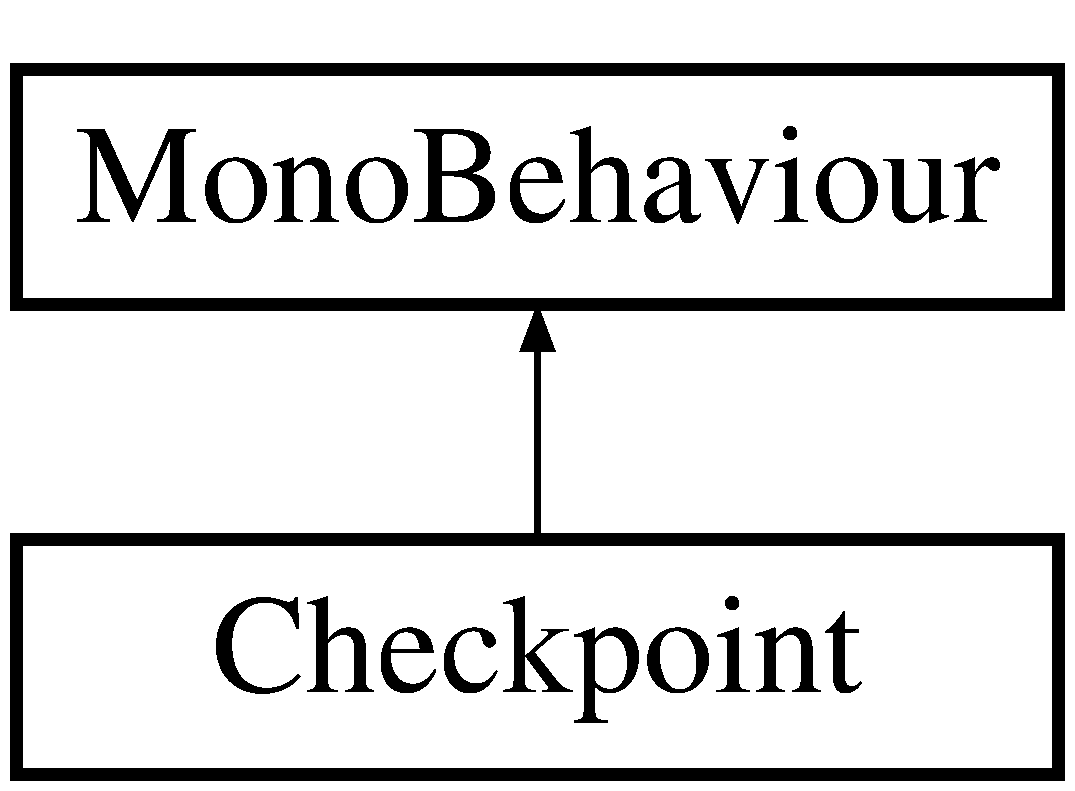
\includegraphics[height=2.000000cm]{class_checkpoint}
\end{center}
\end{figure}
\subsection*{Metody publiczne}
\begin{DoxyCompactItemize}
\item 
void {\bf Awake} ()
\begin{DoxyCompactList}\small\item\em Tworzenie listy listenerów obsługujących respawn obiektów wraz z graczem w kolejnych checkpointach. \end{DoxyCompactList}\item 
void {\bf Player\+Hit\+Checkpoint} ()
\begin{DoxyCompactList}\small\item\em Uruchomienie metody Player\+Hit\+Checkpoint\+Co, z aktualną wartością bonusu czasowego jako argumentem. \end{DoxyCompactList}\item 
void {\bf Player\+Left\+Checkpoint} ()
\begin{DoxyCompactList}\small\item\em Metoda wywoływana w razie opuszczenia checkpointu (nic nie robi). \end{DoxyCompactList}\item 
void {\bf Spawn\+Player} ({\bf Player} player)
\begin{DoxyCompactList}\small\item\em Respawnowanie gracza w miejscu, w którym znajduje się checkpoint. \end{DoxyCompactList}\item 
void {\bf Assign\+Object\+To\+Checkpoint} ({\bf I\+Player\+Respawn\+Listener} listener)
\begin{DoxyCompactList}\small\item\em Przydzielanie obiektów do checkpointów, które mają się zrespawnować po respawnie gracza. \end{DoxyCompactList}\end{DoxyCompactItemize}


\subsection{Opis szczegółowy}
Klasa odpowiedzialna za respawn gracza w danym checkpoincie. 



\subsection{Dokumentacja funkcji składowych}
\index{Checkpoint@{Checkpoint}!Assign\+Object\+To\+Checkpoint@{Assign\+Object\+To\+Checkpoint}}
\index{Assign\+Object\+To\+Checkpoint@{Assign\+Object\+To\+Checkpoint}!Checkpoint@{Checkpoint}}
\subsubsection[{Assign\+Object\+To\+Checkpoint(\+I\+Player\+Respawn\+Listener listener)}]{\setlength{\rightskip}{0pt plus 5cm}void Checkpoint.\+Assign\+Object\+To\+Checkpoint (
\begin{DoxyParamCaption}
\item[{{\bf I\+Player\+Respawn\+Listener}}]{listener}
\end{DoxyParamCaption}
)}\label{class_checkpoint_a5fa902f81ee5c306bc6ed25d9ce62185}


Przydzielanie obiektów do checkpointów, które mają się zrespawnować po respawnie gracza. 


\begin{DoxyParams}{Parametry}
{\em listener} & \\
\hline
\end{DoxyParams}
\index{Checkpoint@{Checkpoint}!Awake@{Awake}}
\index{Awake@{Awake}!Checkpoint@{Checkpoint}}
\subsubsection[{Awake()}]{\setlength{\rightskip}{0pt plus 5cm}void Checkpoint.\+Awake (
\begin{DoxyParamCaption}
{}
\end{DoxyParamCaption}
)}\label{class_checkpoint_af3783fddf42967c30cfd022dfc582d79}


Tworzenie listy listenerów obsługujących respawn obiektów wraz z graczem w kolejnych checkpointach. 

\index{Checkpoint@{Checkpoint}!Player\+Hit\+Checkpoint@{Player\+Hit\+Checkpoint}}
\index{Player\+Hit\+Checkpoint@{Player\+Hit\+Checkpoint}!Checkpoint@{Checkpoint}}
\subsubsection[{Player\+Hit\+Checkpoint()}]{\setlength{\rightskip}{0pt plus 5cm}void Checkpoint.\+Player\+Hit\+Checkpoint (
\begin{DoxyParamCaption}
{}
\end{DoxyParamCaption}
)}\label{class_checkpoint_a9dda39b239a45089698864768a4bd11c}


Uruchomienie metody Player\+Hit\+Checkpoint\+Co, z aktualną wartością bonusu czasowego jako argumentem. 

\index{Checkpoint@{Checkpoint}!Player\+Left\+Checkpoint@{Player\+Left\+Checkpoint}}
\index{Player\+Left\+Checkpoint@{Player\+Left\+Checkpoint}!Checkpoint@{Checkpoint}}
\subsubsection[{Player\+Left\+Checkpoint()}]{\setlength{\rightskip}{0pt plus 5cm}void Checkpoint.\+Player\+Left\+Checkpoint (
\begin{DoxyParamCaption}
{}
\end{DoxyParamCaption}
)}\label{class_checkpoint_a732b4b8be74672d68c011e03016270cd}


Metoda wywoływana w razie opuszczenia checkpointu (nic nie robi). 

\index{Checkpoint@{Checkpoint}!Spawn\+Player@{Spawn\+Player}}
\index{Spawn\+Player@{Spawn\+Player}!Checkpoint@{Checkpoint}}
\subsubsection[{Spawn\+Player(\+Player player)}]{\setlength{\rightskip}{0pt plus 5cm}void Checkpoint.\+Spawn\+Player (
\begin{DoxyParamCaption}
\item[{{\bf Player}}]{player}
\end{DoxyParamCaption}
)}\label{class_checkpoint_a3b56b2963f8df54bee9e5647428bfcd5}


Respawnowanie gracza w miejscu, w którym znajduje się checkpoint. 


\begin{DoxyParams}{Parametry}
{\em player} & \\
\hline
\end{DoxyParams}


Dokumentacja dla tej klasy została wygenerowana z pliku\+:\begin{DoxyCompactItemize}
\item 
C\+:/\+Users/\+Paul/\+Projects/\+Unity\+Game/\+Projekt/\+Assets/\+Code/Checkpoint.\+cs\end{DoxyCompactItemize}

\section{Dokumentacja klasy Controller\+Parameters2\+D}
\label{class_controller_parameters2_d}\index{Controller\+Parameters2\+D@{Controller\+Parameters2\+D}}


klasa \doxyref{Controller\+Parameters2\+D}{str.}{class_controller_parameters2_d}  


\subsection*{Typy publiczne}
\begin{DoxyCompactItemize}
\item 
enum {\bf Jump\+Behavior} \{ {\bfseries Can\+Jump\+On\+Ground}, 
{\bfseries Can\+Jump\+Anywhere}, 
{\bfseries Cant\+Jump}
 \}\label{class_controller_parameters2_d_a2838d319f4380bc1120750fdff3dd22f}
\begin{DoxyCompactList}\small\item\em Czy mozna wykonac skok i w jakich okolicznosciach. \end{DoxyCompactList}
\end{DoxyCompactItemize}
\subsection*{Atrybuty publiczne}
\begin{DoxyCompactItemize}
\item 
Vector2 {\bf Max\+Velocity} = new Vector2(float.\+Max\+Value, float.\+Max\+Value)\label{class_controller_parameters2_d_a06ebe9f5ed4fb8a39c1ed11f36659b2b}

\begin{DoxyCompactList}\small\item\em Ustawienie maksymalnej predkosci gracza. \end{DoxyCompactList}\item 
float {\bf Slope\+Limit} = 30
\begin{DoxyCompactList}\small\item\em Slope\+Limit. \end{DoxyCompactList}\item 
float {\bf Gravity} = -\/25f\label{class_controller_parameters2_d_ae83e87db83f426c232a43dd15e30fb38}

\begin{DoxyCompactList}\small\item\em Grawitacja. \end{DoxyCompactList}\item 
{\bf Jump\+Behavior} {\bf Jump\+Restrictions}\label{class_controller_parameters2_d_aa709ad9bce9649d1fbb6e5146c141325}

\begin{DoxyCompactList}\small\item\em Jump\+Restrictions. \end{DoxyCompactList}\item 
float {\bf Jump\+Frequency} = .\+25f\label{class_controller_parameters2_d_ac1215bef2bee5c3e555b92e79ad447cb}

\begin{DoxyCompactList}\small\item\em Częstotliwość skoku. \end{DoxyCompactList}\item 
float {\bf Jump\+Magnitude} = 12\label{class_controller_parameters2_d_ae92dcce1c474adc687bcfa45ca02ae27}

\begin{DoxyCompactList}\small\item\em Siła skoku. \end{DoxyCompactList}\end{DoxyCompactItemize}


\subsection{Opis szczegółowy}
klasa \doxyref{Controller\+Parameters2\+D}{str.}{class_controller_parameters2_d} 



\subsection{Dokumentacja atrybutów składowych}
\index{Controller\+Parameters2\+D@{Controller\+Parameters2\+D}!Slope\+Limit@{Slope\+Limit}}
\index{Slope\+Limit@{Slope\+Limit}!Controller\+Parameters2\+D@{Controller\+Parameters2\+D}}
\subsubsection[{Slope\+Limit}]{\setlength{\rightskip}{0pt plus 5cm}float Controller\+Parameters2\+D.\+Slope\+Limit = 30}\label{class_controller_parameters2_d_ae706235bff2d67da0d71293bef2ea8d1}


Slope\+Limit. 

Nie mozna wejsc na teren o nachyleniu wiekszym od 30 stopni. Ustalenie grawitacji, dopusczalnej czestotliwosci skokow i ich sily. 

Dokumentacja dla tej klasy została wygenerowana z pliku\+:\begin{DoxyCompactItemize}
\item 
C\+:/\+Users/\+Paul/\+Projects/\+Unity\+Game/\+Projekt/\+Assets/\+Code/Controller\+Parameters2\+D.\+cs\end{DoxyCompactItemize}

\section{Dokumentacja klasy Controller\+Physics\+Volume2\+D}
\label{class_controller_physics_volume2_d}\index{Controller\+Physics\+Volume2\+D@{Controller\+Physics\+Volume2\+D}}


klasa \doxyref{Controller\+Physics\+Volume2\+D}{str.}{class_controller_physics_volume2_d}  


Diagram dziedziczenia dla Controller\+Physics\+Volume2\+D\begin{figure}[H]
\begin{center}
\leavevmode
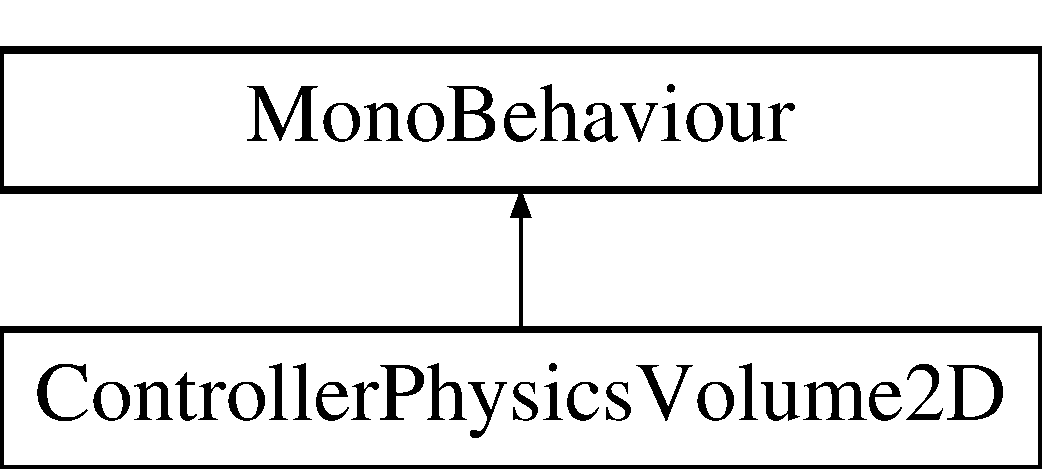
\includegraphics[height=2.000000cm]{class_controller_physics_volume2_d}
\end{center}
\end{figure}
\subsection*{Atrybuty publiczne}
\begin{DoxyCompactItemize}
\item 
{\bf Controller\+Parameters2\+D} {\bf Parameters}
\begin{DoxyCompactList}\small\item\em Uzywane przy zmianie srodowiska w jakim jest gracz (np. na wode), co wplywa na parametry kontrolera. \end{DoxyCompactList}\end{DoxyCompactItemize}


\subsection{Opis szczegółowy}
klasa \doxyref{Controller\+Physics\+Volume2\+D}{str.}{class_controller_physics_volume2_d} 



\subsection{Dokumentacja atrybutów składowych}
\index{Controller\+Physics\+Volume2\+D@{Controller\+Physics\+Volume2\+D}!Parameters@{Parameters}}
\index{Parameters@{Parameters}!Controller\+Physics\+Volume2\+D@{Controller\+Physics\+Volume2\+D}}
\subsubsection[{Parameters}]{\setlength{\rightskip}{0pt plus 5cm}{\bf Controller\+Parameters2\+D} Controller\+Physics\+Volume2\+D.\+Parameters}\label{class_controller_physics_volume2_d_a57a01a60fe2b7a3ab0bd7808211a42b7}


Uzywane przy zmianie srodowiska w jakim jest gracz (np. na wode), co wplywa na parametry kontrolera. 



Dokumentacja dla tej klasy została wygenerowana z pliku\+:\begin{DoxyCompactItemize}
\item 
C\+:/\+Users/\+Paul/\+Projects/\+Unity\+Game/\+Projekt/\+Assets/\+Code/Controller\+Physics\+Volume2\+D.\+cs\end{DoxyCompactItemize}

\section{Dokumentacja klasy Controller\+State2\+D}
\label{class_controller_state2_d}\index{Controller\+State2\+D@{Controller\+State2\+D}}


klasa \doxyref{Controller\+State2\+D}{str.}{class_controller_state2_d}  


\subsection*{Metody publiczne}
\begin{DoxyCompactItemize}
\item 
void {\bf Reset} ()
\begin{DoxyCompactList}\small\item\em Reset stanu \end{DoxyCompactList}\item 
override string {\bf To\+String} ()
\begin{DoxyCompactList}\small\item\em Debug \end{DoxyCompactList}\end{DoxyCompactItemize}
\subsection*{Właściwości}
\begin{DoxyCompactItemize}
\item 
bool {\bf Is\+Colliding\+Right}\hspace{0.3cm}{\ttfamily  [get, set]}
\begin{DoxyCompactList}\small\item\em Kolizja z prawej strony \end{DoxyCompactList}\item 
bool {\bf Is\+Colliding\+Left}\hspace{0.3cm}{\ttfamily  [get, set]}
\begin{DoxyCompactList}\small\item\em Kolizja z lewej strony \end{DoxyCompactList}\item 
bool {\bf Is\+Colliding\+Above}\hspace{0.3cm}{\ttfamily  [get, set]}
\begin{DoxyCompactList}\small\item\em Kolizja powyżej \end{DoxyCompactList}\item 
bool {\bf Is\+Colliding\+Below}\hspace{0.3cm}{\ttfamily  [get, set]}
\begin{DoxyCompactList}\small\item\em Kolizja z poniżej \end{DoxyCompactList}\item 
bool {\bf Is\+Moving\+Down\+Slope}\hspace{0.3cm}{\ttfamily  [get, set]}
\begin{DoxyCompactList}\small\item\em Kolizja ruch po pochyłej (dół) \end{DoxyCompactList}\item 
bool {\bf Is\+Moving\+Up\+Slope}\hspace{0.3cm}{\ttfamily  [get, set]}
\begin{DoxyCompactList}\small\item\em Kolizja ruch po pochyłej (góra) \end{DoxyCompactList}\item 
bool {\bf Is\+Grounded}\hspace{0.3cm}{\ttfamily  [get]}
\begin{DoxyCompactList}\small\item\em Kolizja ziemia \end{DoxyCompactList}\item 
float {\bf Slope\+Angle}\hspace{0.3cm}{\ttfamily  [get, set]}
\begin{DoxyCompactList}\small\item\em Kąt pochyłej \end{DoxyCompactList}\item 
bool {\bf Has\+Collisions}\hspace{0.3cm}{\ttfamily  [get]}
\begin{DoxyCompactList}\small\item\em Kolizja jakakolwiek \end{DoxyCompactList}\end{DoxyCompactItemize}


\subsection{Opis szczegółowy}
klasa \doxyref{Controller\+State2\+D}{str.}{class_controller_state2_d} 



\subsection{Dokumentacja funkcji składowych}
\index{Controller\+State2\+D@{Controller\+State2\+D}!Reset@{Reset}}
\index{Reset@{Reset}!Controller\+State2\+D@{Controller\+State2\+D}}
\subsubsection[{Reset()}]{\setlength{\rightskip}{0pt plus 5cm}void Controller\+State2\+D.\+Reset (
\begin{DoxyParamCaption}
{}
\end{DoxyParamCaption}
)}\label{class_controller_state2_d_a227682256d3eabc548dcd982cbcb7aef}


Reset stanu 

\index{Controller\+State2\+D@{Controller\+State2\+D}!To\+String@{To\+String}}
\index{To\+String@{To\+String}!Controller\+State2\+D@{Controller\+State2\+D}}
\subsubsection[{To\+String()}]{\setlength{\rightskip}{0pt plus 5cm}override string Controller\+State2\+D.\+To\+String (
\begin{DoxyParamCaption}
{}
\end{DoxyParamCaption}
)}\label{class_controller_state2_d_af8f1803156a41e5a8ca0c7c6a7f12865}


Debug 



\subsection{Dokumentacja właściwości}
\index{Controller\+State2\+D@{Controller\+State2\+D}!Has\+Collisions@{Has\+Collisions}}
\index{Has\+Collisions@{Has\+Collisions}!Controller\+State2\+D@{Controller\+State2\+D}}
\subsubsection[{Has\+Collisions}]{\setlength{\rightskip}{0pt plus 5cm}bool Controller\+State2\+D.\+Has\+Collisions\hspace{0.3cm}{\ttfamily [get]}}\label{class_controller_state2_d_a81b74ffe89ca998f186dfcc01cd74a80}


Kolizja jakakolwiek 

\index{Controller\+State2\+D@{Controller\+State2\+D}!Is\+Colliding\+Above@{Is\+Colliding\+Above}}
\index{Is\+Colliding\+Above@{Is\+Colliding\+Above}!Controller\+State2\+D@{Controller\+State2\+D}}
\subsubsection[{Is\+Colliding\+Above}]{\setlength{\rightskip}{0pt plus 5cm}bool Controller\+State2\+D.\+Is\+Colliding\+Above\hspace{0.3cm}{\ttfamily [get]}, {\ttfamily [set]}}\label{class_controller_state2_d_a31e26c803a9fa52216eccaf2adb94b67}


Kolizja powyżej 

\index{Controller\+State2\+D@{Controller\+State2\+D}!Is\+Colliding\+Below@{Is\+Colliding\+Below}}
\index{Is\+Colliding\+Below@{Is\+Colliding\+Below}!Controller\+State2\+D@{Controller\+State2\+D}}
\subsubsection[{Is\+Colliding\+Below}]{\setlength{\rightskip}{0pt plus 5cm}bool Controller\+State2\+D.\+Is\+Colliding\+Below\hspace{0.3cm}{\ttfamily [get]}, {\ttfamily [set]}}\label{class_controller_state2_d_ac23ed207ad3b8225b8cdea0505165c8a}


Kolizja z poniżej 

\index{Controller\+State2\+D@{Controller\+State2\+D}!Is\+Colliding\+Left@{Is\+Colliding\+Left}}
\index{Is\+Colliding\+Left@{Is\+Colliding\+Left}!Controller\+State2\+D@{Controller\+State2\+D}}
\subsubsection[{Is\+Colliding\+Left}]{\setlength{\rightskip}{0pt plus 5cm}bool Controller\+State2\+D.\+Is\+Colliding\+Left\hspace{0.3cm}{\ttfamily [get]}, {\ttfamily [set]}}\label{class_controller_state2_d_a4774afc53858b57f6016e1fb620268c4}


Kolizja z lewej strony 

\index{Controller\+State2\+D@{Controller\+State2\+D}!Is\+Colliding\+Right@{Is\+Colliding\+Right}}
\index{Is\+Colliding\+Right@{Is\+Colliding\+Right}!Controller\+State2\+D@{Controller\+State2\+D}}
\subsubsection[{Is\+Colliding\+Right}]{\setlength{\rightskip}{0pt plus 5cm}bool Controller\+State2\+D.\+Is\+Colliding\+Right\hspace{0.3cm}{\ttfamily [get]}, {\ttfamily [set]}}\label{class_controller_state2_d_ab415da9f261852bca7ba1ec57adf41bb}


Kolizja z prawej strony 

\index{Controller\+State2\+D@{Controller\+State2\+D}!Is\+Grounded@{Is\+Grounded}}
\index{Is\+Grounded@{Is\+Grounded}!Controller\+State2\+D@{Controller\+State2\+D}}
\subsubsection[{Is\+Grounded}]{\setlength{\rightskip}{0pt plus 5cm}bool Controller\+State2\+D.\+Is\+Grounded\hspace{0.3cm}{\ttfamily [get]}}\label{class_controller_state2_d_a895b129b6c8f95dd3aef68d9342a14d8}


Kolizja ziemia 

\index{Controller\+State2\+D@{Controller\+State2\+D}!Is\+Moving\+Down\+Slope@{Is\+Moving\+Down\+Slope}}
\index{Is\+Moving\+Down\+Slope@{Is\+Moving\+Down\+Slope}!Controller\+State2\+D@{Controller\+State2\+D}}
\subsubsection[{Is\+Moving\+Down\+Slope}]{\setlength{\rightskip}{0pt plus 5cm}bool Controller\+State2\+D.\+Is\+Moving\+Down\+Slope\hspace{0.3cm}{\ttfamily [get]}, {\ttfamily [set]}}\label{class_controller_state2_d_a813f7c0a080a2b3f784751bb4fa63057}


Kolizja ruch po pochyłej (dół) 

\index{Controller\+State2\+D@{Controller\+State2\+D}!Is\+Moving\+Up\+Slope@{Is\+Moving\+Up\+Slope}}
\index{Is\+Moving\+Up\+Slope@{Is\+Moving\+Up\+Slope}!Controller\+State2\+D@{Controller\+State2\+D}}
\subsubsection[{Is\+Moving\+Up\+Slope}]{\setlength{\rightskip}{0pt plus 5cm}bool Controller\+State2\+D.\+Is\+Moving\+Up\+Slope\hspace{0.3cm}{\ttfamily [get]}, {\ttfamily [set]}}\label{class_controller_state2_d_ace3f85ee5879533e319143ee09b16f91}


Kolizja ruch po pochyłej (góra) 

\index{Controller\+State2\+D@{Controller\+State2\+D}!Slope\+Angle@{Slope\+Angle}}
\index{Slope\+Angle@{Slope\+Angle}!Controller\+State2\+D@{Controller\+State2\+D}}
\subsubsection[{Slope\+Angle}]{\setlength{\rightskip}{0pt plus 5cm}float Controller\+State2\+D.\+Slope\+Angle\hspace{0.3cm}{\ttfamily [get]}, {\ttfamily [set]}}\label{class_controller_state2_d_a724ea7c59fdf1d3c6f1e8fa80998651a}


Kąt pochyłej 



Dokumentacja dla tej klasy została wygenerowana z pliku\+:\begin{DoxyCompactItemize}
\item 
C\+:/\+Users/\+Paul/\+Projects/\+Unity\+Game/\+Projekt/\+Assets/\+Code/Controller\+State2\+D.\+cs\end{DoxyCompactItemize}

\section{Dokumentacja klasy Finish\+Level}
\label{class_finish_level}\index{Finish\+Level@{Finish\+Level}}


Klasa odpowiedzialna za przejście do następnego poziomu, po wejściu w obszar zmiany poziomu.  


Diagram dziedziczenia dla Finish\+Level\begin{figure}[H]
\begin{center}
\leavevmode
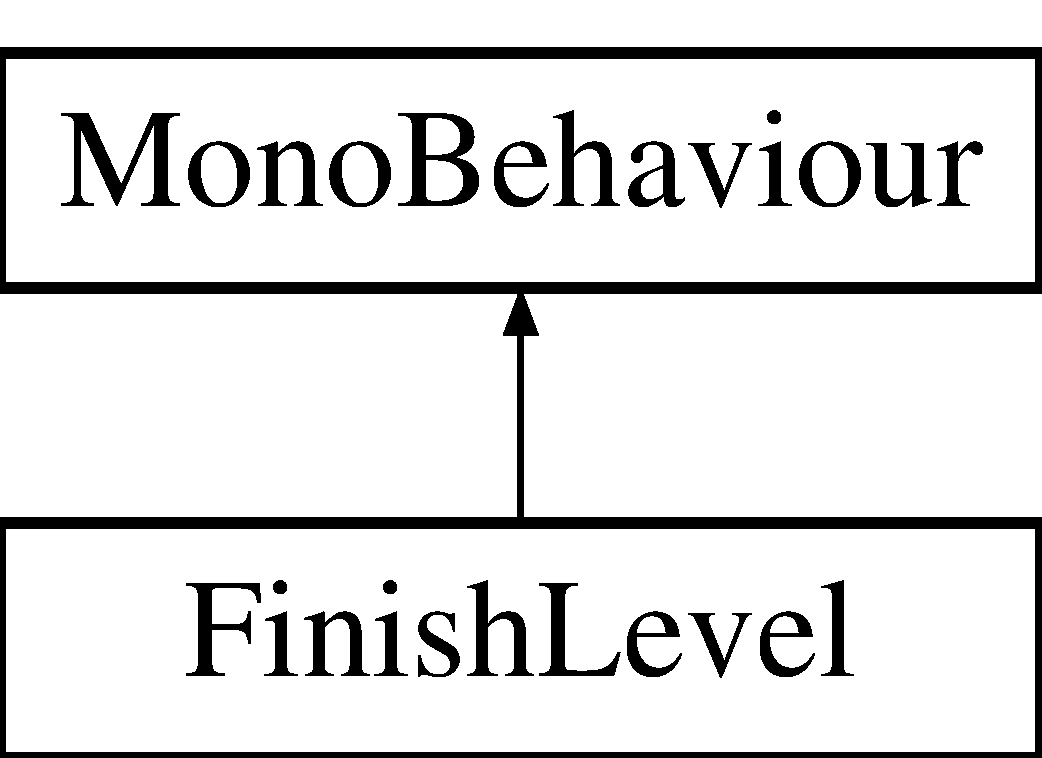
\includegraphics[height=2.000000cm]{class_finish_level}
\end{center}
\end{figure}
\subsection*{Metody publiczne}
\begin{DoxyCompactItemize}
\item 
void {\bfseries On\+Trigger\+Enter2\+D} (Collider2\+D other)\label{class_finish_level_a804424e6504b606f708cd11cd714623e}

\end{DoxyCompactItemize}
\subsection*{Atrybuty publiczne}
\begin{DoxyCompactItemize}
\item 
string {\bfseries Level\+Name}\label{class_finish_level_a29676e91d97a2fb2ab59689b56f609a9}

\end{DoxyCompactItemize}


\subsection{Opis szczegółowy}
Klasa odpowiedzialna za przejście do następnego poziomu, po wejściu w obszar zmiany poziomu. 



Dokumentacja dla tej klasy została wygenerowana z pliku\+:\begin{DoxyCompactItemize}
\item 
C\+:/\+Users/\+Paul/\+Projects/\+Unity\+Game/\+Projekt/\+Assets/\+Code/Finish\+Level.\+cs\end{DoxyCompactItemize}

\section{Dokumentacja klasy Floating\+Text}
\label{class_floating_text}\index{Floating\+Text@{Floating\+Text}}


Klasa odpowiedzialna za wyświetlanie na ekranie gry tekstu informującego o różnych zdarzeniach występujących w czasie rozgrywki.  


Diagram dziedziczenia dla Floating\+Text\begin{figure}[H]
\begin{center}
\leavevmode
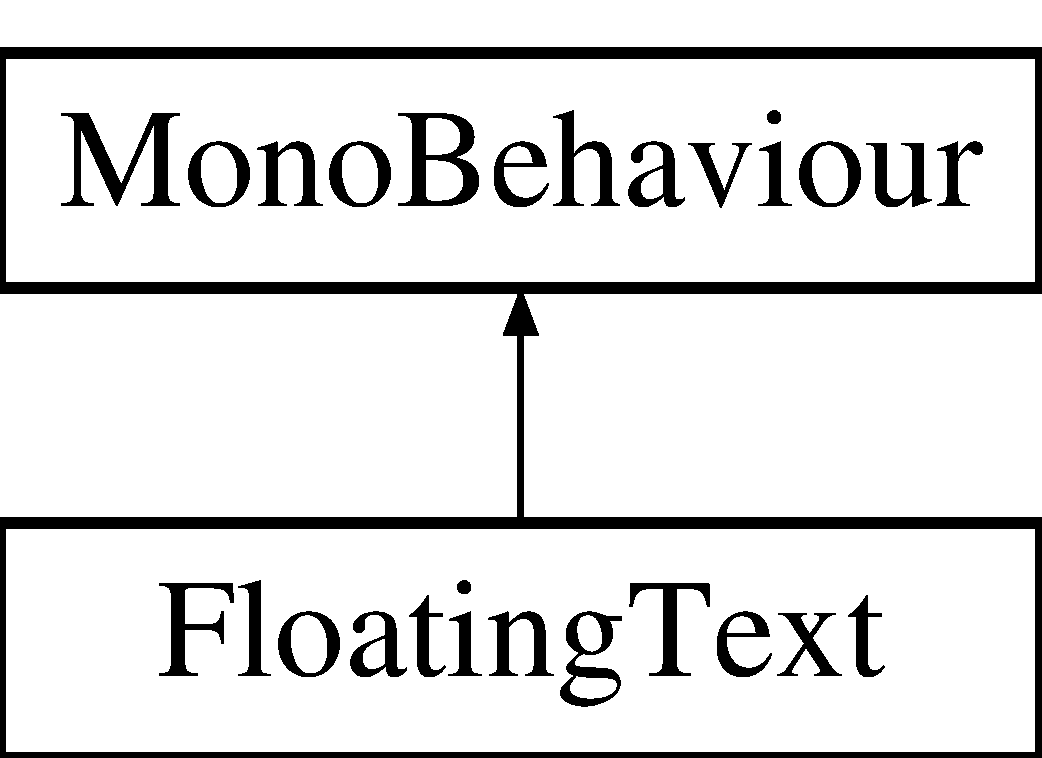
\includegraphics[height=2.000000cm]{class_floating_text}
\end{center}
\end{figure}
\subsection*{Metody publiczne}
\begin{DoxyCompactItemize}
\item 
void {\bf On\+G\+U\+I} ()
\begin{DoxyCompactList}\small\item\em Metoda pokazująca tekst na ekranie oraz usuwająca go. \end{DoxyCompactList}\end{DoxyCompactItemize}
\subsection*{Statyczne metody publiczne}
\begin{DoxyCompactItemize}
\item 
static {\bf Floating\+Text} {\bf Show} (string text, string style, {\bf I\+Floating\+Text\+Positioner} positioner)
\end{DoxyCompactItemize}
\subsection*{Właściwości}
\begin{DoxyCompactItemize}
\item 
string {\bf Text}\hspace{0.3cm}{\ttfamily  [get, set]}\label{class_floating_text_a8f7c9936c710b923c16bf231ac06030f}

\begin{DoxyCompactList}\small\item\em Wyświetlany tekst. \end{DoxyCompactList}\item 
G\+U\+I\+Style {\bf Style}\hspace{0.3cm}{\ttfamily  [get, set]}\label{class_floating_text_a4d9e7743444033595122aa17fad56e97}

\begin{DoxyCompactList}\small\item\em Zmienna stylu interfejsu użytkownika. \end{DoxyCompactList}\end{DoxyCompactItemize}


\subsection{Opis szczegółowy}
Klasa odpowiedzialna za wyświetlanie na ekranie gry tekstu informującego o różnych zdarzeniach występujących w czasie rozgrywki. 



\subsection{Dokumentacja funkcji składowych}
\index{Floating\+Text@{Floating\+Text}!On\+G\+U\+I@{On\+G\+U\+I}}
\index{On\+G\+U\+I@{On\+G\+U\+I}!Floating\+Text@{Floating\+Text}}
\subsubsection[{On\+G\+U\+I()}]{\setlength{\rightskip}{0pt plus 5cm}void Floating\+Text.\+On\+G\+U\+I (
\begin{DoxyParamCaption}
{}
\end{DoxyParamCaption}
)}\label{class_floating_text_a273d9408af60fdd88162447971168f91}


Metoda pokazująca tekst na ekranie oraz usuwająca go. 

Obliczenie wielkości tekstu.

Jeśli wartość zmiennej wskazującej, gdzie ma być wyświetlony tekst jest pusta, niszczony jest obiekt tekstu.

Usunięcie tekstu.

Metoda tworząca tekst na ekranie. \index{Floating\+Text@{Floating\+Text}!Show@{Show}}
\index{Show@{Show}!Floating\+Text@{Floating\+Text}}
\subsubsection[{Show(string text, string style, I\+Floating\+Text\+Positioner positioner)}]{\setlength{\rightskip}{0pt plus 5cm}static {\bf Floating\+Text} Floating\+Text.\+Show (
\begin{DoxyParamCaption}
\item[{string}]{text, }
\item[{string}]{style, }
\item[{{\bf I\+Floating\+Text\+Positioner}}]{positioner}
\end{DoxyParamCaption}
)\hspace{0.3cm}{\ttfamily [static]}}\label{class_floating_text_aec904126f9b38b503a21b498347b3705}
Stworzenie nowego obiektu gry.

Ustawienie stylu tekstu.

Ustawienie miejsca, w którym wyświetlony zostanie tekst.

Ustawienie treści tekstu, która zostanie pokazany. 

Dokumentacja dla tej klasy została wygenerowana z pliku\+:\begin{DoxyCompactItemize}
\item 
C\+:/\+Users/\+Paul/\+Projects/\+Unity\+Game/\+Projekt/\+Assets/\+Code/Floating\+Text.\+cs\end{DoxyCompactItemize}

\section{Dokumentacja klasy Follow\+Object}
\label{class_follow_object}\index{Follow\+Object@{Follow\+Object}}


Klasa zapewnia podążanie pasku za graczem (w odpowiedniej odległości).  


Diagram dziedziczenia dla Follow\+Object\begin{figure}[H]
\begin{center}
\leavevmode
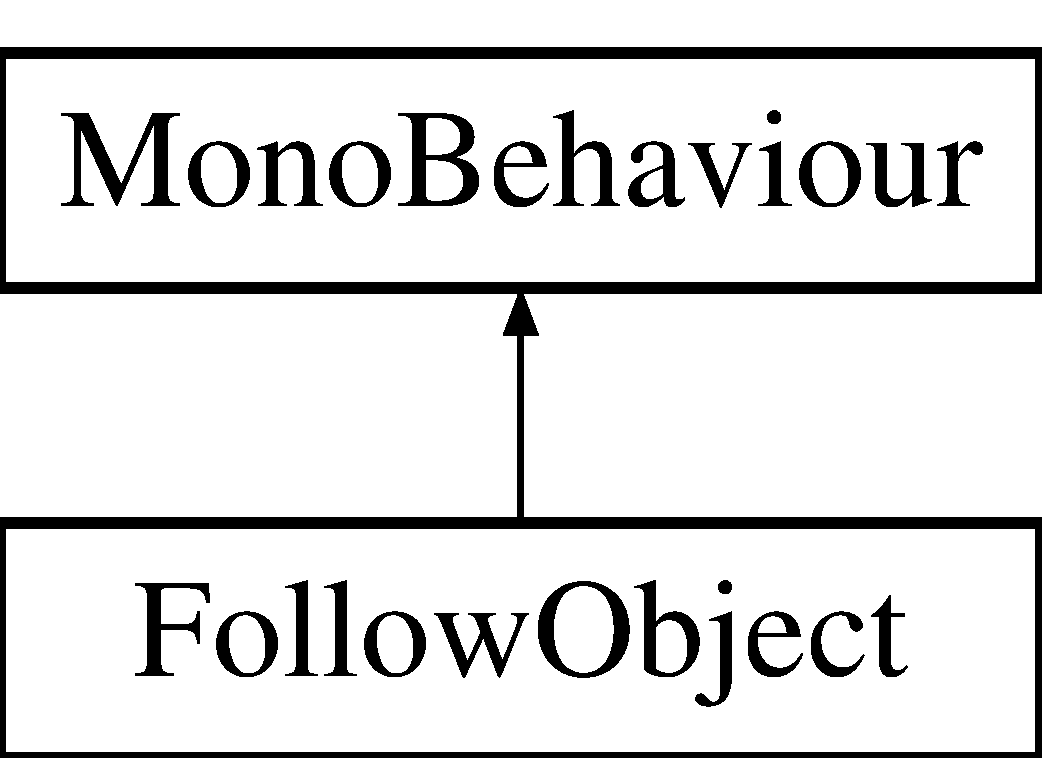
\includegraphics[height=2.000000cm]{class_follow_object}
\end{center}
\end{figure}
\subsection*{Metody publiczne}
\begin{DoxyCompactItemize}
\item 
void {\bf Update} ()
\begin{DoxyCompactList}\small\item\em Aktualizacja położenia pasku zdrowia na podstawie ruchu gracza. \end{DoxyCompactList}\end{DoxyCompactItemize}
\subsection*{Atrybuty publiczne}
\begin{DoxyCompactItemize}
\item 
Vector2 {\bfseries Offset}\label{class_follow_object_a570c760481d19bd4ed4033892797cb62}

\item 
Transform {\bfseries Following}\label{class_follow_object_a6531fc68059005901bccc67fae6d34ec}

\end{DoxyCompactItemize}


\subsection{Opis szczegółowy}
Klasa zapewnia podążanie pasku za graczem (w odpowiedniej odległości). 



\subsection{Dokumentacja funkcji składowych}
\index{Follow\+Object@{Follow\+Object}!Update@{Update}}
\index{Update@{Update}!Follow\+Object@{Follow\+Object}}
\subsubsection[{Update()}]{\setlength{\rightskip}{0pt plus 5cm}void Follow\+Object.\+Update (
\begin{DoxyParamCaption}
{}
\end{DoxyParamCaption}
)}\label{class_follow_object_aea0a99782dd1ab6dc1eeaf9dbe2a3777}


Aktualizacja położenia pasku zdrowia na podstawie ruchu gracza. 



Dokumentacja dla tej klasy została wygenerowana z pliku\+:\begin{DoxyCompactItemize}
\item 
C\+:/\+Users/\+Paul/\+Projects/\+Unity\+Game/\+Projekt/\+Assets/\+Code/Follow\+Object.\+cs\end{DoxyCompactItemize}

\section{Dokumentacja klasy Follow\+Path}
\label{class_follow_path}\index{Follow\+Path@{Follow\+Path}}


klasa \doxyref{Follow\+Path}{str.}{class_follow_path}  


Diagram dziedziczenia dla Follow\+Path\begin{figure}[H]
\begin{center}
\leavevmode
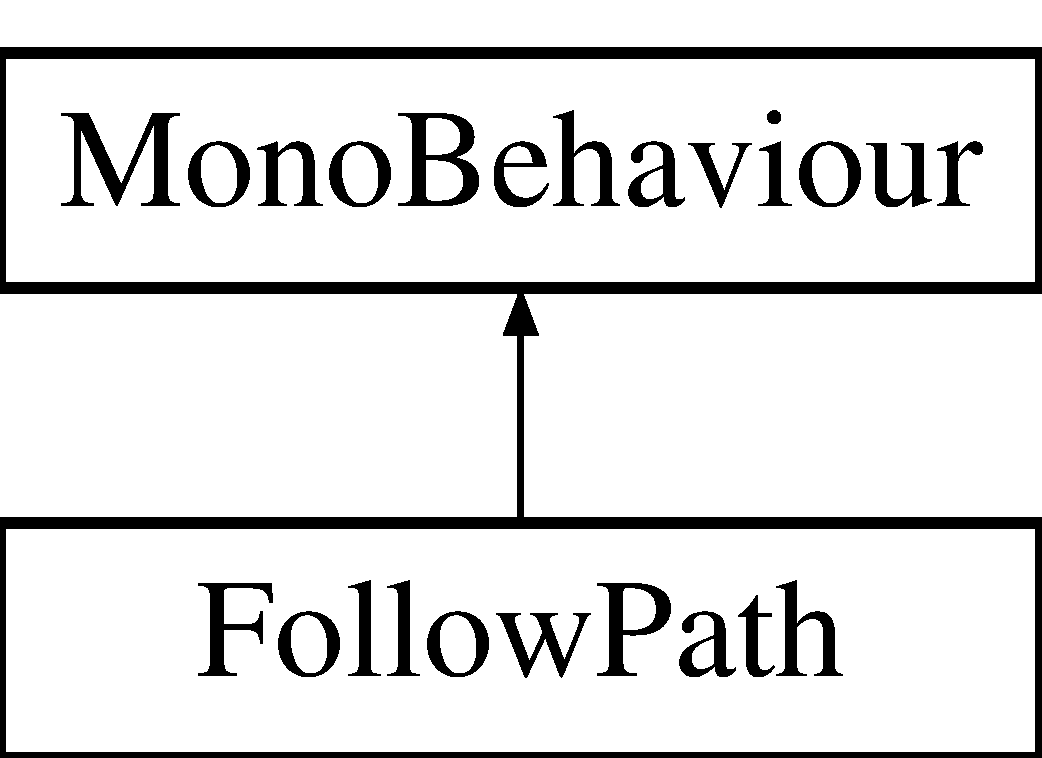
\includegraphics[height=2.000000cm]{class_follow_path}
\end{center}
\end{figure}
\subsection*{Typy publiczne}
\begin{DoxyCompactItemize}
\item 
enum {\bf Follow\+Type} \{ {\bfseries Move\+Towards}, 
{\bfseries Lerp}
 \}\label{class_follow_path_aa15222ed17c7bb53f199e5cb5e5c9cef}
\begin{DoxyCompactList}\small\item\em Wybor trybu ruchu. Lerp -\/ wykorzystujacy interpolacje liniowa. \end{DoxyCompactList}
\end{DoxyCompactItemize}
\subsection*{Metody publiczne}
\begin{DoxyCompactItemize}
\item 
void {\bf Start} ()\label{class_follow_path_a5e1828cf1cf7744c062a58e4a0d29605}

\begin{DoxyCompactList}\small\item\em Inicjalizacja. \end{DoxyCompactList}\item 
void {\bf Update} ()
\end{DoxyCompactItemize}
\subsection*{Atrybuty publiczne}
\begin{DoxyCompactItemize}
\item 
{\bf Follow\+Type} {\bf Type} = Follow\+Type.\+Move\+Towards\label{class_follow_path_a923cc736d703c012d1b6d8874291fa35}

\begin{DoxyCompactList}\small\item\em Typ. \end{DoxyCompactList}\item 
{\bf Path\+Definition} {\bf Path}\label{class_follow_path_a14f4aab3adc712c07ae9a02b87ffb2e3}

\begin{DoxyCompactList}\small\item\em Ścieżka. \end{DoxyCompactList}\item 
float {\bf Speed} = 1\label{class_follow_path_a366b7ad38c7db477e1217ae5c364ac2b}

\begin{DoxyCompactList}\small\item\em Prękość \end{DoxyCompactList}\item 
float {\bf Max\+Distance\+To\+Goal} = .\+1f\label{class_follow_path_a7fd1ef16a8e77196e526d285197ed847}

\begin{DoxyCompactList}\small\item\em Maksymalna odległość \end{DoxyCompactList}\end{DoxyCompactItemize}


\subsection{Opis szczegółowy}
klasa \doxyref{Follow\+Path}{str.}{class_follow_path} 



\subsection{Dokumentacja funkcji składowych}
\index{Follow\+Path@{Follow\+Path}!Update@{Update}}
\index{Update@{Update}!Follow\+Path@{Follow\+Path}}
\subsubsection[{Update()}]{\setlength{\rightskip}{0pt plus 5cm}void Follow\+Path.\+Update (
\begin{DoxyParamCaption}
{}
\end{DoxyParamCaption}
)}\label{class_follow_path_a157ad1da8560085de3542e46050d7183}
Obiekt stworzony bez sciezki, albo ze sciezka ktora nie ma co najmniej jednego punktu.

Argumenty\+: obecna pozycja, pozycja docelowa, predkosc (skalowana przez delta\+Time, aby zapewnic plynnosc animacji).

Sprawdzenie czy osiagnelismy cel i mozemy przemiescic sie do kolejnego punktu. 

Dokumentacja dla tej klasy została wygenerowana z pliku\+:\begin{DoxyCompactItemize}
\item 
C\+:/\+Users/\+Paul/\+Projects/\+Unity\+Game/\+Projekt/\+Assets/\+Code/Follow\+Path.\+cs\end{DoxyCompactItemize}

\section{Dokumentacja klasy From\+World\+Point\+Text\+Positioner}
\label{class_from_world_point_text_positioner}\index{From\+World\+Point\+Text\+Positioner@{From\+World\+Point\+Text\+Positioner}}


Klasa określająca parametry wyświetlanego tekstu w świecie gry.  


Diagram dziedziczenia dla From\+World\+Point\+Text\+Positioner\begin{figure}[H]
\begin{center}
\leavevmode
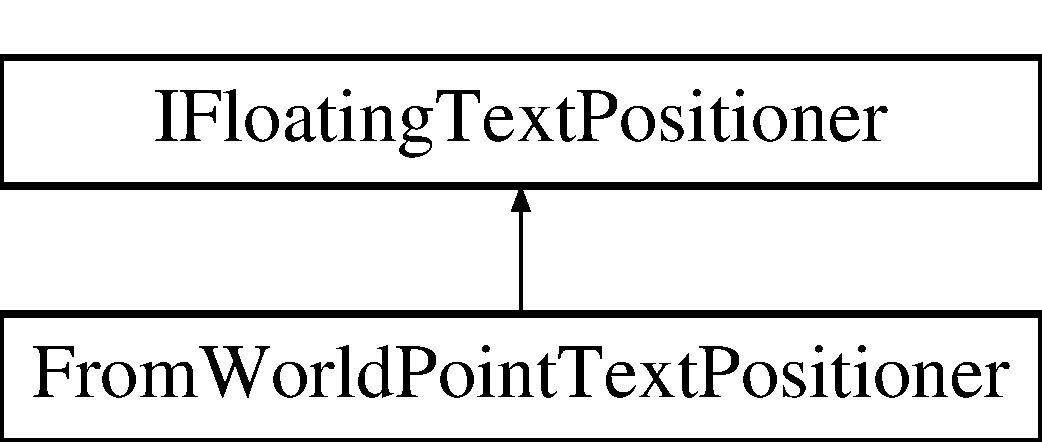
\includegraphics[height=2.000000cm]{class_from_world_point_text_positioner}
\end{center}
\end{figure}
\subsection*{Metody publiczne}
\begin{DoxyCompactItemize}
\item 
{\bf From\+World\+Point\+Text\+Positioner} (Camera Camera, Vector3 world\+Position, float time\+To\+Live, float speed)
\begin{DoxyCompactList}\small\item\em Konstruktor pozycjonera tekstu w grze, przyjmujący jako parametry pozycję tekstu w świecie gry, obiekt kamery, czas, przez jaki ma być wyświetlany tekst i prędkość poruszania się tekstu. \end{DoxyCompactList}\item 
bool {\bf Get\+Position} (ref Vector2 position, G\+U\+I\+Content content, Vector2 size)
\begin{DoxyCompactList}\small\item\em Metoda mówiąca \doxyref{Floating\+Text}{str.}{class_floating_text}, czy dalej wyświetlać tekst. Ustawia również współrzędne tekstu w grze. \end{DoxyCompactList}\end{DoxyCompactItemize}


\subsection{Opis szczegółowy}
Klasa określająca parametry wyświetlanego tekstu w świecie gry. 



\subsection{Dokumentacja konstruktora i destruktora}
\index{From\+World\+Point\+Text\+Positioner@{From\+World\+Point\+Text\+Positioner}!From\+World\+Point\+Text\+Positioner@{From\+World\+Point\+Text\+Positioner}}
\index{From\+World\+Point\+Text\+Positioner@{From\+World\+Point\+Text\+Positioner}!From\+World\+Point\+Text\+Positioner@{From\+World\+Point\+Text\+Positioner}}
\subsubsection[{From\+World\+Point\+Text\+Positioner(\+Camera Camera, Vector3 world\+Position, float time\+To\+Live, float speed)}]{\setlength{\rightskip}{0pt plus 5cm}From\+World\+Point\+Text\+Positioner.\+From\+World\+Point\+Text\+Positioner (
\begin{DoxyParamCaption}
\item[{Camera}]{Camera, }
\item[{Vector3}]{world\+Position, }
\item[{float}]{time\+To\+Live, }
\item[{float}]{speed}
\end{DoxyParamCaption}
)}\label{class_from_world_point_text_positioner_aa9ba697a3e48cde9e486d184f8df532b}


Konstruktor pozycjonera tekstu w grze, przyjmujący jako parametry pozycję tekstu w świecie gry, obiekt kamery, czas, przez jaki ma być wyświetlany tekst i prędkość poruszania się tekstu. 


\begin{DoxyParams}{Parametry}
{\em Camera} & \\
\hline
{\em world\+Position} & \\
\hline
{\em time\+To\+Live} & \\
\hline
{\em speed} & \\
\hline
\end{DoxyParams}


\subsection{Dokumentacja funkcji składowych}
\index{From\+World\+Point\+Text\+Positioner@{From\+World\+Point\+Text\+Positioner}!Get\+Position@{Get\+Position}}
\index{Get\+Position@{Get\+Position}!From\+World\+Point\+Text\+Positioner@{From\+World\+Point\+Text\+Positioner}}
\subsubsection[{Get\+Position(ref Vector2 position, G\+U\+I\+Content content, Vector2 size)}]{\setlength{\rightskip}{0pt plus 5cm}bool From\+World\+Point\+Text\+Positioner.\+Get\+Position (
\begin{DoxyParamCaption}
\item[{ref Vector2}]{position, }
\item[{G\+U\+I\+Content}]{content, }
\item[{Vector2}]{size}
\end{DoxyParamCaption}
)}\label{class_from_world_point_text_positioner_aa42b82c9124f7d4aa1dcc6874af031d2}


Metoda mówiąca \doxyref{Floating\+Text}{str.}{class_floating_text}, czy dalej wyświetlać tekst. Ustawia również współrzędne tekstu w grze. 


\begin{DoxyParams}{Parametry}
{\em position} & \\
\hline
{\em content} & \\
\hline
{\em size} & \\
\hline
\end{DoxyParams}
\begin{DoxyReturn}{Zwraca}

\end{DoxyReturn}
Jeśli podczas wyświetlania tekstu (dana klatka), upłynie czas życia napisu, metoda zwraca false. Klasa \doxyref{Floating\+Text}{str.}{class_floating_text} niszczy wtedy tekst.

Środkujemy tekst na współrzędnych świata. 

Implementuje {\bf I\+Floating\+Text\+Positioner} \doxyref{}{str.}{interface_i_floating_text_positioner}.



Dokumentacja dla tej klasy została wygenerowana z pliku\+:\begin{DoxyCompactItemize}
\item 
C\+:/\+Users/\+Paul/\+Projects/\+Unity\+Game/\+Projekt/\+Assets/\+Code/From\+World\+Point\+Text\+Positione.\+cs\end{DoxyCompactItemize}

\section{Dokumentacja klasy Game\+Hud}
\label{class_game_hud}\index{Game\+Hud@{Game\+Hud}}


Klasa odpowiedzialna za wyświetlanie komunikatu o zdobytych punktach za zebranie gwiazdek i dojście do nowego checkpointu (bonus czasowy).  


Diagram dziedziczenia dla Game\+Hud\begin{figure}[H]
\begin{center}
\leavevmode
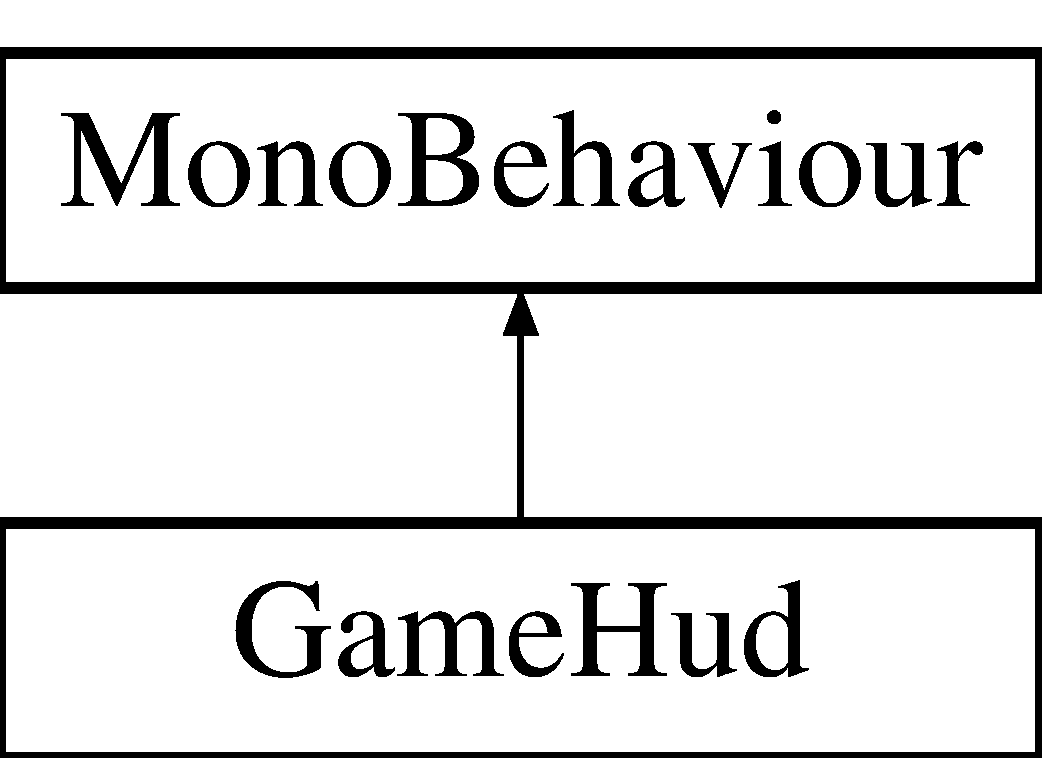
\includegraphics[height=2.000000cm]{class_game_hud}
\end{center}
\end{figure}
\subsection*{Metody publiczne}
\begin{DoxyCompactItemize}
\item 
void {\bfseries On\+G\+U\+I} ()\label{class_game_hud_a9b3a0ab6fe0867aafb05c2aab0f9590c}

\end{DoxyCompactItemize}
\subsection*{Atrybuty publiczne}
\begin{DoxyCompactItemize}
\item 
G\+U\+I\+Skin {\bfseries Skin}\label{class_game_hud_a40a8fcd77291bc5080b12cfc89f28a4a}

\end{DoxyCompactItemize}


\subsection{Opis szczegółowy}
Klasa odpowiedzialna za wyświetlanie komunikatu o zdobytych punktach za zebranie gwiazdek i dojście do nowego checkpointu (bonus czasowy). 



Dokumentacja dla tej klasy została wygenerowana z pliku\+:\begin{DoxyCompactItemize}
\item 
C\+:/\+Users/\+Paul/\+Projects/\+Unity\+Game/\+Projekt/\+Assets/\+Code/Game\+Hud.\+cs\end{DoxyCompactItemize}

\section{Dokumentacja klasy Game\+Manager}
\label{class_game_manager}\index{Game\+Manager@{Game\+Manager}}


Klasa odpowiedzialna za naliczanie i resetowanie punktów podczas gry.  


\subsection*{Metody publiczne}
\begin{DoxyCompactItemize}
\item 
void {\bf Reset} ()
\begin{DoxyCompactList}\small\item\em Wyzerowanie punktów. \end{DoxyCompactList}\item 
void {\bf Reset\+Points} (int points)
\begin{DoxyCompactList}\small\item\em Ustawienie ilości punktów na wartość podaną w parametrze. \end{DoxyCompactList}\item 
void {\bf Add\+Points} (int points\+To\+Add)
\begin{DoxyCompactList}\small\item\em Dodanie punktów. \end{DoxyCompactList}\end{DoxyCompactItemize}
\subsection*{Właściwości}
\begin{DoxyCompactItemize}
\item 
static {\bf Game\+Manager} {\bfseries Instance}\hspace{0.3cm}{\ttfamily  [get]}\label{class_game_manager_ad3e717f4fb0f378b969f4457de81f23e}

\item 
int {\bfseries Points}\hspace{0.3cm}{\ttfamily  [get]}\label{class_game_manager_ad6b14d4dcf3b37f9e3c626bb4fff6755}

\end{DoxyCompactItemize}


\subsection{Opis szczegółowy}
Klasa odpowiedzialna za naliczanie i resetowanie punktów podczas gry. 



\subsection{Dokumentacja funkcji składowych}
\index{Game\+Manager@{Game\+Manager}!Add\+Points@{Add\+Points}}
\index{Add\+Points@{Add\+Points}!Game\+Manager@{Game\+Manager}}
\subsubsection[{Add\+Points(int points\+To\+Add)}]{\setlength{\rightskip}{0pt plus 5cm}void Game\+Manager.\+Add\+Points (
\begin{DoxyParamCaption}
\item[{int}]{points\+To\+Add}
\end{DoxyParamCaption}
)}\label{class_game_manager_ac88cd8451e52e90ae426711153e5cb7f}


Dodanie punktów. 


\begin{DoxyParams}{Parametry}
{\em points\+To\+Add} & \\
\hline
\end{DoxyParams}
\index{Game\+Manager@{Game\+Manager}!Reset@{Reset}}
\index{Reset@{Reset}!Game\+Manager@{Game\+Manager}}
\subsubsection[{Reset()}]{\setlength{\rightskip}{0pt plus 5cm}void Game\+Manager.\+Reset (
\begin{DoxyParamCaption}
{}
\end{DoxyParamCaption}
)}\label{class_game_manager_a50401d6452934e7e126cd24bd5e04e79}


Wyzerowanie punktów. 

\index{Game\+Manager@{Game\+Manager}!Reset\+Points@{Reset\+Points}}
\index{Reset\+Points@{Reset\+Points}!Game\+Manager@{Game\+Manager}}
\subsubsection[{Reset\+Points(int points)}]{\setlength{\rightskip}{0pt plus 5cm}void Game\+Manager.\+Reset\+Points (
\begin{DoxyParamCaption}
\item[{int}]{points}
\end{DoxyParamCaption}
)}\label{class_game_manager_ae2303bf083aa49a662e0c85c5259bfba}


Ustawienie ilości punktów na wartość podaną w parametrze. 


\begin{DoxyParams}{Parametry}
{\em points} & \\
\hline
\end{DoxyParams}


Dokumentacja dla tej klasy została wygenerowana z pliku\+:\begin{DoxyCompactItemize}
\item 
C\+:/\+Users/\+Paul/\+Projects/\+Unity\+Game/\+Projekt/\+Assets/\+Code/Game\+Manager.\+cs\end{DoxyCompactItemize}

\section{Dokumentacja klasy Give\+Damage\+To\+Player}
\label{class_give_damage_to_player}\index{Give\+Damage\+To\+Player@{Give\+Damage\+To\+Player}}


Klasa odpowiedzialna za zadawanie obrażeń graczowi przez dany obiekt.  


Diagram dziedziczenia dla Give\+Damage\+To\+Player\begin{figure}[H]
\begin{center}
\leavevmode
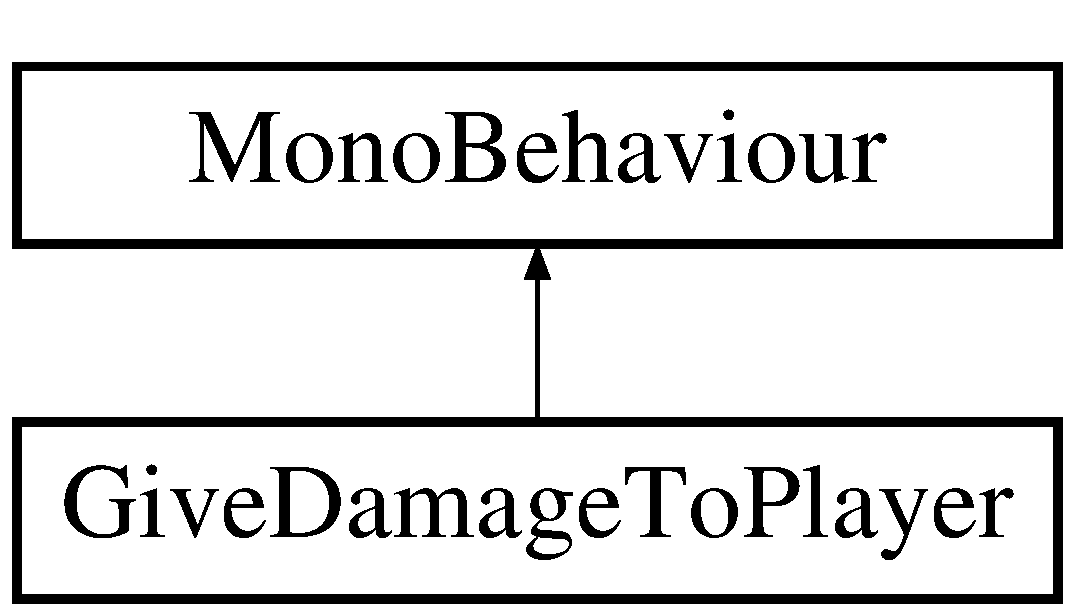
\includegraphics[height=2.000000cm]{class_give_damage_to_player}
\end{center}
\end{figure}
\subsection*{Metody publiczne}
\begin{DoxyCompactItemize}
\item 
void {\bf Late\+Update} ()
\begin{DoxyCompactList}\small\item\em Aktualizacja położenia obiektu. \end{DoxyCompactList}\item 
void {\bf On\+Trigger\+Enter2\+D} (Collider2\+D other)
\begin{DoxyCompactList}\small\item\em Odebranie punktów zdrowia gracza po zderzeniu z Colliderem2\+D obiektu, oraz ustawienie lekkiego \char`\"{}odrzutu\char`\"{} gracza w tył po otrzymaniu obrażeń. \end{DoxyCompactList}\end{DoxyCompactItemize}
\subsection*{Atrybuty publiczne}
\begin{DoxyCompactItemize}
\item 
int {\bf Damage\+To\+Give} = 10
\begin{DoxyCompactList}\small\item\em Domyślna wartośc obrażeń zadawana graczowi. \end{DoxyCompactList}\end{DoxyCompactItemize}


\subsection{Opis szczegółowy}
Klasa odpowiedzialna za zadawanie obrażeń graczowi przez dany obiekt. 



\subsection{Dokumentacja funkcji składowych}
\index{Give\+Damage\+To\+Player@{Give\+Damage\+To\+Player}!Late\+Update@{Late\+Update}}
\index{Late\+Update@{Late\+Update}!Give\+Damage\+To\+Player@{Give\+Damage\+To\+Player}}
\subsubsection[{Late\+Update()}]{\setlength{\rightskip}{0pt plus 5cm}void Give\+Damage\+To\+Player.\+Late\+Update (
\begin{DoxyParamCaption}
{}
\end{DoxyParamCaption}
)}\label{class_give_damage_to_player_a10a14435668cc395091402be6cb85ed7}


Aktualizacja położenia obiektu. 

\index{Give\+Damage\+To\+Player@{Give\+Damage\+To\+Player}!On\+Trigger\+Enter2\+D@{On\+Trigger\+Enter2\+D}}
\index{On\+Trigger\+Enter2\+D@{On\+Trigger\+Enter2\+D}!Give\+Damage\+To\+Player@{Give\+Damage\+To\+Player}}
\subsubsection[{On\+Trigger\+Enter2\+D(\+Collider2\+D other)}]{\setlength{\rightskip}{0pt plus 5cm}void Give\+Damage\+To\+Player.\+On\+Trigger\+Enter2\+D (
\begin{DoxyParamCaption}
\item[{Collider2\+D}]{other}
\end{DoxyParamCaption}
)}\label{class_give_damage_to_player_a4fbe3591f30889e39a822ea7b0b37149}


Odebranie punktów zdrowia gracza po zderzeniu z Colliderem2\+D obiektu, oraz ustawienie lekkiego \char`\"{}odrzutu\char`\"{} gracza w tył po otrzymaniu obrażeń. 


\begin{DoxyParams}{Parametry}
{\em other} & \\
\hline
\end{DoxyParams}


\subsection{Dokumentacja atrybutów składowych}
\index{Give\+Damage\+To\+Player@{Give\+Damage\+To\+Player}!Damage\+To\+Give@{Damage\+To\+Give}}
\index{Damage\+To\+Give@{Damage\+To\+Give}!Give\+Damage\+To\+Player@{Give\+Damage\+To\+Player}}
\subsubsection[{Damage\+To\+Give}]{\setlength{\rightskip}{0pt plus 5cm}int Give\+Damage\+To\+Player.\+Damage\+To\+Give = 10}\label{class_give_damage_to_player_a77c01e1c1f269957c6b5230334334578}


Domyślna wartośc obrażeń zadawana graczowi. 



Dokumentacja dla tej klasy została wygenerowana z pliku\+:\begin{DoxyCompactItemize}
\item 
C\+:/\+Users/\+Paul/\+Projects/\+Unity\+Game/\+Projekt/\+Assets/\+Code/Give\+Damage\+To\+Player.\+cs\end{DoxyCompactItemize}

\section{Dokumentacja klasy Give\+Health}
\label{class_give_health}\index{Give\+Health@{Give\+Health}}


Klasa odpowiadająca za dodanie punktów zdrowia gracza po zebraniu apteczki.  


Diagram dziedziczenia dla Give\+Health\begin{figure}[H]
\begin{center}
\leavevmode
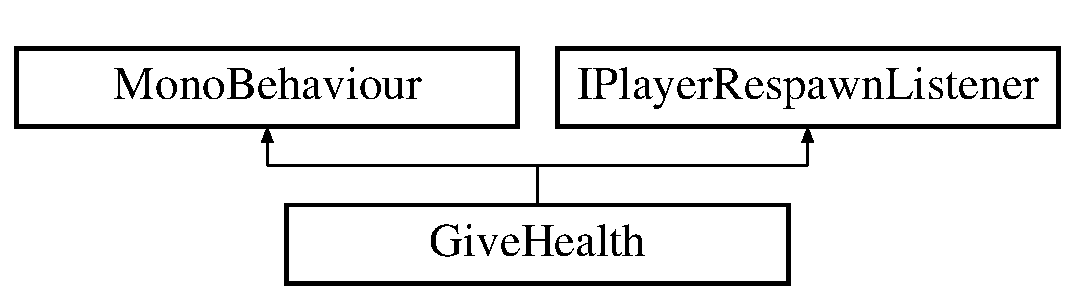
\includegraphics[height=2.000000cm]{class_give_health}
\end{center}
\end{figure}
\subsection*{Metody publiczne}
\begin{DoxyCompactItemize}
\item 
void {\bf On\+Trigger\+Enter2\+D} (Collider2\+D other)
\begin{DoxyCompactList}\small\item\em Metoda uruchamiana po zebraniu apteczki. \end{DoxyCompactList}\item 
void {\bf On\+Player\+Respawn\+In\+This\+Checkpoint} ({\bf Checkpoint} checkpoint, {\bf Player} player)
\begin{DoxyCompactList}\small\item\em Respawnowanie apteczki po powrocie do ostatniego checkpointu. \end{DoxyCompactList}\end{DoxyCompactItemize}
\subsection*{Atrybuty publiczne}
\begin{DoxyCompactItemize}
\item 
Game\+Object {\bf Effect}
\begin{DoxyCompactList}\small\item\em Efekt graficzny towarzyszący zebraniu apteczki. \end{DoxyCompactList}\item 
int {\bf Health\+To\+Give}
\begin{DoxyCompactList}\small\item\em Ilośc punktów zdrowia dodawanych przez zebranie apteczki. \end{DoxyCompactList}\end{DoxyCompactItemize}


\subsection{Opis szczegółowy}
Klasa odpowiadająca za dodanie punktów zdrowia gracza po zebraniu apteczki. 



\subsection{Dokumentacja funkcji składowych}
\index{Give\+Health@{Give\+Health}!On\+Player\+Respawn\+In\+This\+Checkpoint@{On\+Player\+Respawn\+In\+This\+Checkpoint}}
\index{On\+Player\+Respawn\+In\+This\+Checkpoint@{On\+Player\+Respawn\+In\+This\+Checkpoint}!Give\+Health@{Give\+Health}}
\subsubsection[{On\+Player\+Respawn\+In\+This\+Checkpoint(\+Checkpoint checkpoint, Player player)}]{\setlength{\rightskip}{0pt plus 5cm}void Give\+Health.\+On\+Player\+Respawn\+In\+This\+Checkpoint (
\begin{DoxyParamCaption}
\item[{{\bf Checkpoint}}]{checkpoint, }
\item[{{\bf Player}}]{player}
\end{DoxyParamCaption}
)}\label{class_give_health_a53c1f61540ebcd9c2ae44537b309a1a1}


Respawnowanie apteczki po powrocie do ostatniego checkpointu. 


\begin{DoxyParams}{Parametry}
{\em checkpoint} & \\
\hline
{\em player} & \\
\hline
\end{DoxyParams}


Implementuje {\bf I\+Player\+Respawn\+Listener} \doxyref{}{str.}{interface_i_player_respawn_listener}.

\index{Give\+Health@{Give\+Health}!On\+Trigger\+Enter2\+D@{On\+Trigger\+Enter2\+D}}
\index{On\+Trigger\+Enter2\+D@{On\+Trigger\+Enter2\+D}!Give\+Health@{Give\+Health}}
\subsubsection[{On\+Trigger\+Enter2\+D(\+Collider2\+D other)}]{\setlength{\rightskip}{0pt plus 5cm}void Give\+Health.\+On\+Trigger\+Enter2\+D (
\begin{DoxyParamCaption}
\item[{Collider2\+D}]{other}
\end{DoxyParamCaption}
)}\label{class_give_health_a6ba8edc28aa1e0f4d3918bcf1d231a00}


Metoda uruchamiana po zebraniu apteczki. 


\begin{DoxyParams}{Parametry}
{\em other} & \\
\hline
\end{DoxyParams}
Dodanie punktów zdrowia.

Zaincijowanie efektu graficznego.

Usunięcie apteczki po jej zebraniu ze świata gry w Unity. 

\subsection{Dokumentacja atrybutów składowych}
\index{Give\+Health@{Give\+Health}!Effect@{Effect}}
\index{Effect@{Effect}!Give\+Health@{Give\+Health}}
\subsubsection[{Effect}]{\setlength{\rightskip}{0pt plus 5cm}Game\+Object Give\+Health.\+Effect}\label{class_give_health_a3b40fdd032931e918c636505222f0a6b}


Efekt graficzny towarzyszący zebraniu apteczki. 

\index{Give\+Health@{Give\+Health}!Health\+To\+Give@{Health\+To\+Give}}
\index{Health\+To\+Give@{Health\+To\+Give}!Give\+Health@{Give\+Health}}
\subsubsection[{Health\+To\+Give}]{\setlength{\rightskip}{0pt plus 5cm}int Give\+Health.\+Health\+To\+Give}\label{class_give_health_aa4ac9c92c64cc4c4d88a3acff8abab85}


Ilośc punktów zdrowia dodawanych przez zebranie apteczki. 



Dokumentacja dla tej klasy została wygenerowana z pliku\+:\begin{DoxyCompactItemize}
\item 
C\+:/\+Users/\+Paul/\+Projects/\+Unity\+Game/\+Projekt/\+Assets/\+Code/Give\+Health.\+cs\end{DoxyCompactItemize}

\section{Dokumentacja klasy Health\+Bar}
\label{class_health_bar}\index{Health\+Bar@{Health\+Bar}}


Klasa pasku zdrowia pojawiającego się nad graczem.  


Diagram dziedziczenia dla Health\+Bar\begin{figure}[H]
\begin{center}
\leavevmode
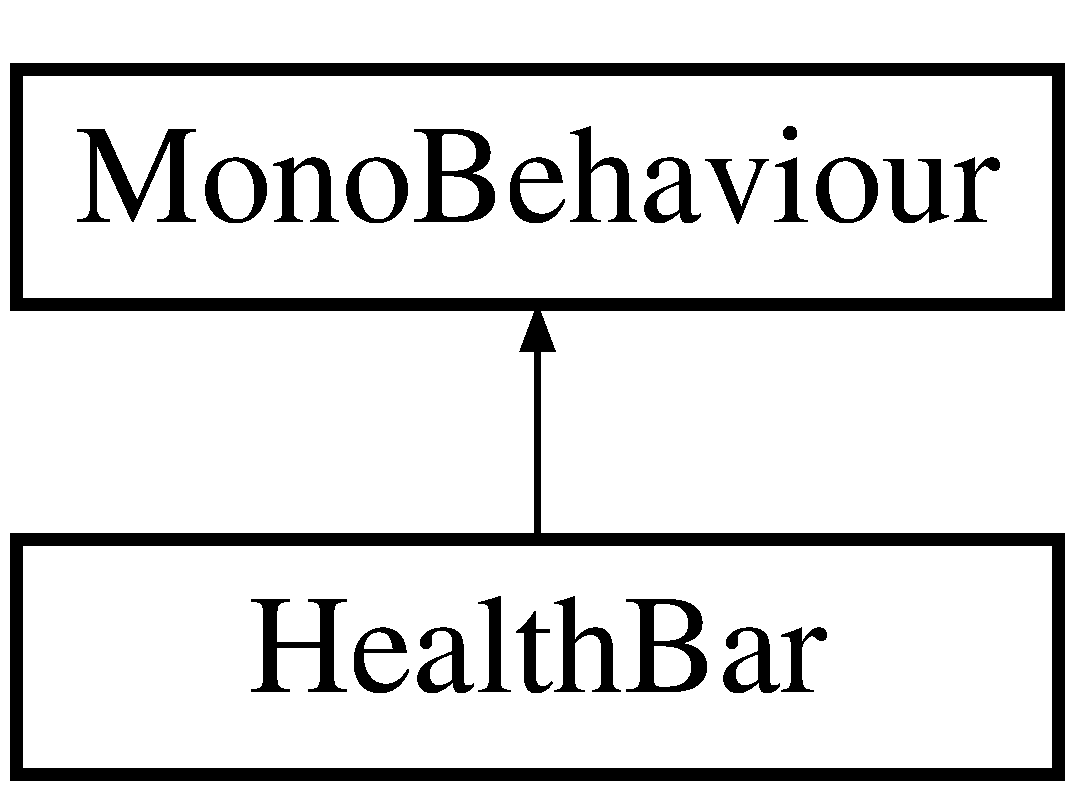
\includegraphics[height=2.000000cm]{class_health_bar}
\end{center}
\end{figure}
\subsection*{Metody publiczne}
\begin{DoxyCompactItemize}
\item 
void {\bf Update} ()
\begin{DoxyCompactList}\small\item\em Aktualizacja punktów zdrowia gracza oraz odpowiadającego koloru. \end{DoxyCompactList}\end{DoxyCompactItemize}
\subsection*{Atrybuty publiczne}
\begin{DoxyCompactItemize}
\item 
{\bf Player} {\bfseries Player}\label{class_health_bar_ab10e19888af476521d8670c9b3f7e714}

\item 
Transform {\bfseries Foreground\+Sprite}\label{class_health_bar_a847748e2e7f8258d45a60ceca229443b}

\item 
Sprite\+Renderer {\bfseries Foreground\+Renderer}\label{class_health_bar_acb0f75afdd7dbca7e1b162ee3809d0b4}

\item 
Color {\bf Max\+Health\+Color} = new Color(255 / 255f, 63 / 255f, 63 / 255f)
\begin{DoxyCompactList}\small\item\em Ustawienie koloru maksymalnej wartości zdrowia na niebieski. \end{DoxyCompactList}\item 
Color {\bf Min\+Health\+Color} = new Color(64 / 255f, 137 / 255f, 255 / 255f)
\begin{DoxyCompactList}\small\item\em Ustawienie koloru minimalnej wartości zdrowia na czerwony. \end{DoxyCompactList}\end{DoxyCompactItemize}


\subsection{Opis szczegółowy}
Klasa pasku zdrowia pojawiającego się nad graczem. 



\subsection{Dokumentacja funkcji składowych}
\index{Health\+Bar@{Health\+Bar}!Update@{Update}}
\index{Update@{Update}!Health\+Bar@{Health\+Bar}}
\subsubsection[{Update()}]{\setlength{\rightskip}{0pt plus 5cm}void Health\+Bar.\+Update (
\begin{DoxyParamCaption}
{}
\end{DoxyParamCaption}
)}\label{class_health_bar_a5a9ddff350a7f337e71a8466cde4ef7f}


Aktualizacja punktów zdrowia gracza oraz odpowiadającego koloru. 



\subsection{Dokumentacja atrybutów składowych}
\index{Health\+Bar@{Health\+Bar}!Max\+Health\+Color@{Max\+Health\+Color}}
\index{Max\+Health\+Color@{Max\+Health\+Color}!Health\+Bar@{Health\+Bar}}
\subsubsection[{Max\+Health\+Color}]{\setlength{\rightskip}{0pt plus 5cm}Color Health\+Bar.\+Max\+Health\+Color = new Color(255 / 255f, 63 / 255f, 63 / 255f)}\label{class_health_bar_ab8d1e8e6cfa0b873f00dbf3a5142dadb}


Ustawienie koloru maksymalnej wartości zdrowia na niebieski. 

\index{Health\+Bar@{Health\+Bar}!Min\+Health\+Color@{Min\+Health\+Color}}
\index{Min\+Health\+Color@{Min\+Health\+Color}!Health\+Bar@{Health\+Bar}}
\subsubsection[{Min\+Health\+Color}]{\setlength{\rightskip}{0pt plus 5cm}Color Health\+Bar.\+Min\+Health\+Color = new Color(64 / 255f, 137 / 255f, 255 / 255f)}\label{class_health_bar_a082780005764c17dda95b689ee1a414f}


Ustawienie koloru minimalnej wartości zdrowia na czerwony. 



Dokumentacja dla tej klasy została wygenerowana z pliku\+:\begin{DoxyCompactItemize}
\item 
C\+:/\+Users/\+Paul/\+Projects/\+Unity\+Game/\+Projekt/\+Assets/\+Code/Health\+Bar.\+cs\end{DoxyCompactItemize}

\section{Dokumentacja interfejsu I\+Floating\+Text\+Positioner}
\label{interface_i_floating_text_positioner}\index{I\+Floating\+Text\+Positioner@{I\+Floating\+Text\+Positioner}}


Interfejs z metodą pozwalającą pobrać położenie tekstu wyświetlanego na ekranie.  


Diagram dziedziczenia dla I\+Floating\+Text\+Positioner\begin{figure}[H]
\begin{center}
\leavevmode
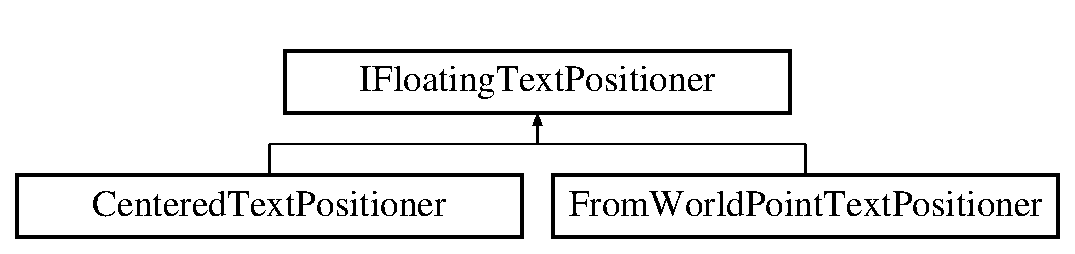
\includegraphics[height=2.000000cm]{interface_i_floating_text_positioner}
\end{center}
\end{figure}
\subsection*{Metody publiczne}
\begin{DoxyCompactItemize}
\item 
bool {\bfseries Get\+Position} (ref Vector2 position, G\+U\+I\+Content content, Vector2 size)\label{interface_i_floating_text_positioner_af8540a70c6c4e7b71f85bf77f9821724}

\end{DoxyCompactItemize}


\subsection{Opis szczegółowy}
Interfejs z metodą pozwalającą pobrać położenie tekstu wyświetlanego na ekranie. 



Dokumentacja dla tego interfejsu została wygenerowana z pliku\+:\begin{DoxyCompactItemize}
\item 
C\+:/\+Users/\+Paul/\+Projects/\+Unity\+Game/\+Projekt/\+Assets/\+Code/I\+Floating\+Text\+Positioner.\+cs\end{DoxyCompactItemize}

\section{Dokumentacja klasy Insta\+Kill}
\label{class_insta_kill}\index{Insta\+Kill@{Insta\+Kill}}


Klasa odpowiedzialna za zabicie gracza, gdy napotka na Collider2\+D danego obiektu.  


Diagram dziedziczenia dla Insta\+Kill\begin{figure}[H]
\begin{center}
\leavevmode
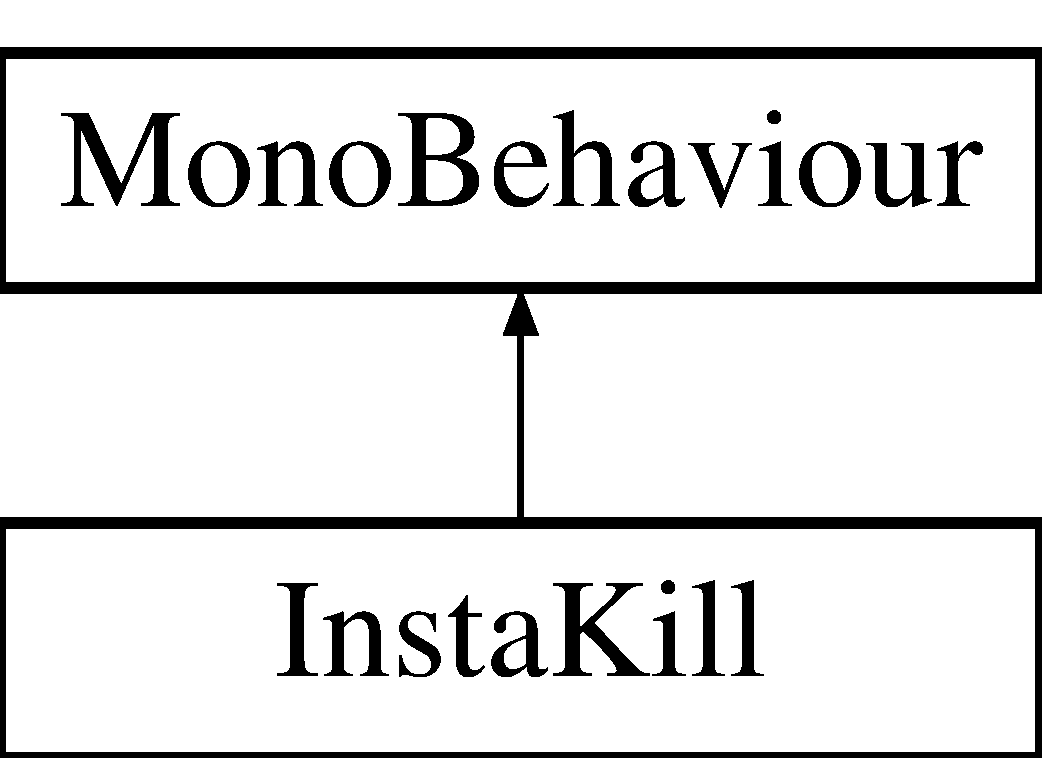
\includegraphics[height=2.000000cm]{class_insta_kill}
\end{center}
\end{figure}
\subsection*{Metody publiczne}
\begin{DoxyCompactItemize}
\item 
void {\bfseries On\+Trigger\+Enter2\+D} (Collider2\+D other)\label{class_insta_kill_aca897e3b9eee1c18c493e73d9c52ffe7}

\end{DoxyCompactItemize}


\subsection{Opis szczegółowy}
Klasa odpowiedzialna za zabicie gracza, gdy napotka na Collider2\+D danego obiektu. 



Dokumentacja dla tej klasy została wygenerowana z pliku\+:\begin{DoxyCompactItemize}
\item 
C\+:/\+Users/\+Paul/\+Projects/\+Unity\+Game/\+Projekt/\+Assets/\+Code/Insta\+Kill.\+cs\end{DoxyCompactItemize}

\section{Dokumentacja interfejsu I\+Player\+Respawn\+Listener}
\label{interface_i_player_respawn_listener}\index{I\+Player\+Respawn\+Listener@{I\+Player\+Respawn\+Listener}}


Interfejs odpowiedzialny za zrespawnowanie gracza w danym checkpoincie.  


Diagram dziedziczenia dla I\+Player\+Respawn\+Listener\begin{figure}[H]
\begin{center}
\leavevmode
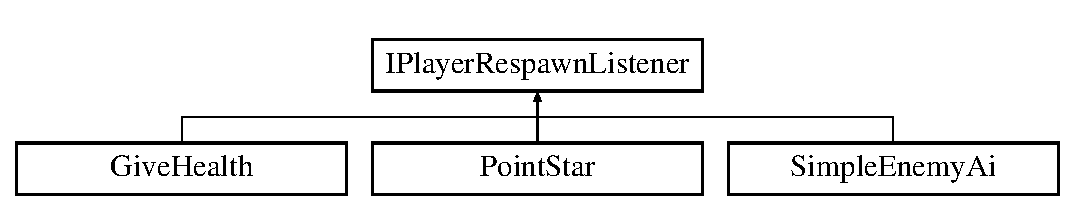
\includegraphics[height=2.000000cm]{interface_i_player_respawn_listener}
\end{center}
\end{figure}
\subsection*{Metody publiczne}
\begin{DoxyCompactItemize}
\item 
void {\bfseries On\+Player\+Respawn\+In\+This\+Checkpoint} ({\bf Checkpoint} checkpoint, {\bf Player} player)\label{interface_i_player_respawn_listener_a3b16a7bd96d7d13af5efcb1cd403d44f}

\end{DoxyCompactItemize}


\subsection{Opis szczegółowy}
Interfejs odpowiedzialny za zrespawnowanie gracza w danym checkpoincie. 



Dokumentacja dla tego interfejsu została wygenerowana z pliku\+:\begin{DoxyCompactItemize}
\item 
C\+:/\+Users/\+Paul/\+Projects/\+Unity\+Game/\+Projekt/\+Assets/\+Code/I\+Player\+Respawn\+Listener.\+cs\end{DoxyCompactItemize}

\section{Dokumentacja interfejsu I\+Take\+Damage}
\label{interface_i_take_damage}\index{I\+Take\+Damage@{I\+Take\+Damage}}


Interfejs posiadający funkcją przyjmowania obrażeń o podanej wartości, zadanych przez dany obiekt.  


Diagram dziedziczenia dla I\+Take\+Damage\begin{figure}[H]
\begin{center}
\leavevmode
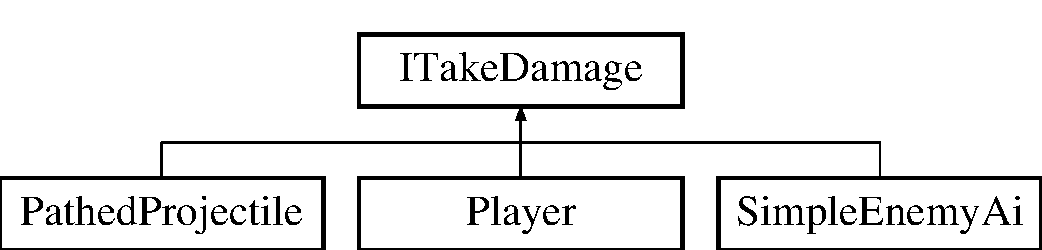
\includegraphics[height=2.000000cm]{interface_i_take_damage}
\end{center}
\end{figure}
\subsection*{Metody publiczne}
\begin{DoxyCompactItemize}
\item 
void {\bfseries Take\+Damage} (int damage, Game\+Object instigator)\label{interface_i_take_damage_a433efa6ef27b7969d7799b46c1ec1949}

\end{DoxyCompactItemize}


\subsection{Opis szczegółowy}
Interfejs posiadający funkcją przyjmowania obrażeń o podanej wartości, zadanych przez dany obiekt. 



Dokumentacja dla tego interfejsu została wygenerowana z pliku\+:\begin{DoxyCompactItemize}
\item 
C\+:/\+Users/\+Paul/\+Projects/\+Unity\+Game/\+Projekt/\+Assets/\+Code/I\+Take\+Damage.\+cs\end{DoxyCompactItemize}

\section{Dokumentacja klasy Jump\+Platform}
\label{class_jump_platform}\index{Jump\+Platform@{Jump\+Platform}}


klasa \doxyref{Jump\+Platform}{str.}{class_jump_platform}  


Diagram dziedziczenia dla Jump\+Platform\begin{figure}[H]
\begin{center}
\leavevmode
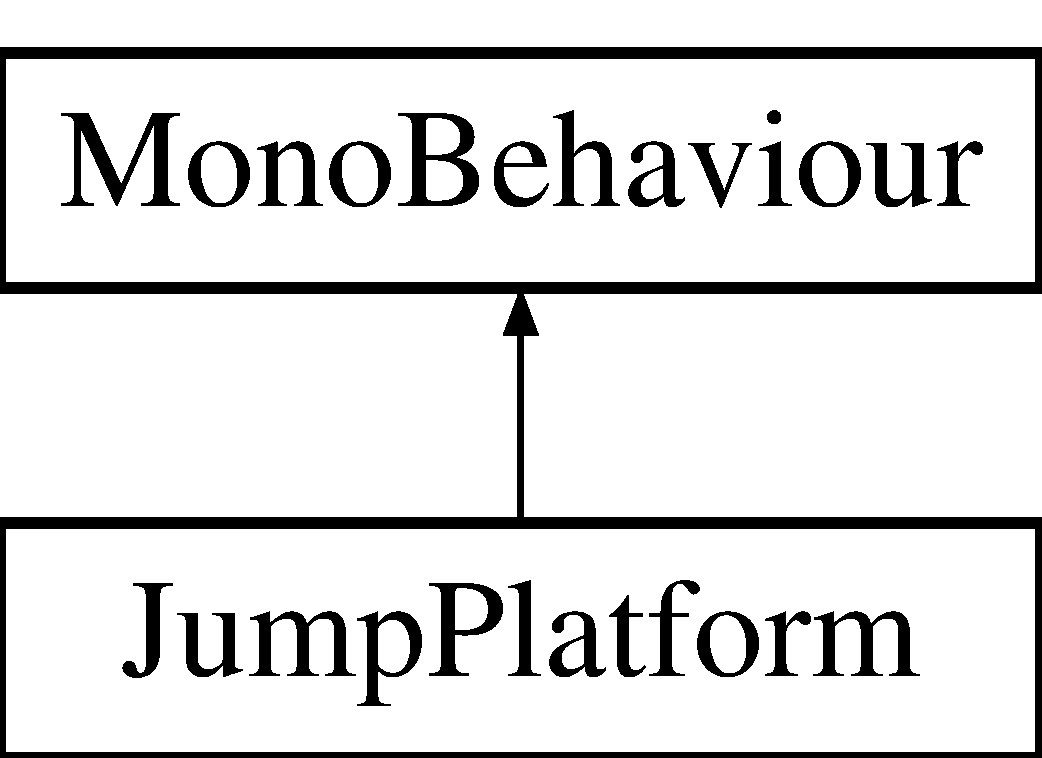
\includegraphics[height=2.000000cm]{class_jump_platform}
\end{center}
\end{figure}
\subsection*{Metody publiczne}
\begin{DoxyCompactItemize}
\item 
void {\bf Controller\+Enter2\+D} ({\bf Character\+Controller2\+D} controller)\label{class_jump_platform_ad1e3b06d092b641e4ef9e773aba1de6d}

\begin{DoxyCompactList}\small\item\em Ustalenie Jump\+Magnitude. \end{DoxyCompactList}\end{DoxyCompactItemize}
\subsection*{Atrybuty publiczne}
\begin{DoxyCompactItemize}
\item 
float {\bf Jump\+Magnitude} = 20\label{class_jump_platform_a089d1fb7693297d093994570c338ad75}

\begin{DoxyCompactList}\small\item\em Ustalenie sily skoku. \end{DoxyCompactList}\item 
Audio\+Clip {\bfseries Jump\+Sound}\label{class_jump_platform_a29c6e5195a52670627fdc77debb32d41}

\end{DoxyCompactItemize}


\subsection{Opis szczegółowy}
klasa \doxyref{Jump\+Platform}{str.}{class_jump_platform} 



Dokumentacja dla tej klasy została wygenerowana z pliku\+:\begin{DoxyCompactItemize}
\item 
C\+:/\+Users/\+Paul/\+Projects/\+Unity\+Game/\+Projekt/\+Assets/\+Code/Jump\+Platform.\+cs\end{DoxyCompactItemize}

\section{Dokumentacja klasy Level\+Manager}
\label{class_level_manager}\index{Level\+Manager@{Level\+Manager}}
Diagram dziedziczenia dla Level\+Manager\begin{figure}[H]
\begin{center}
\leavevmode
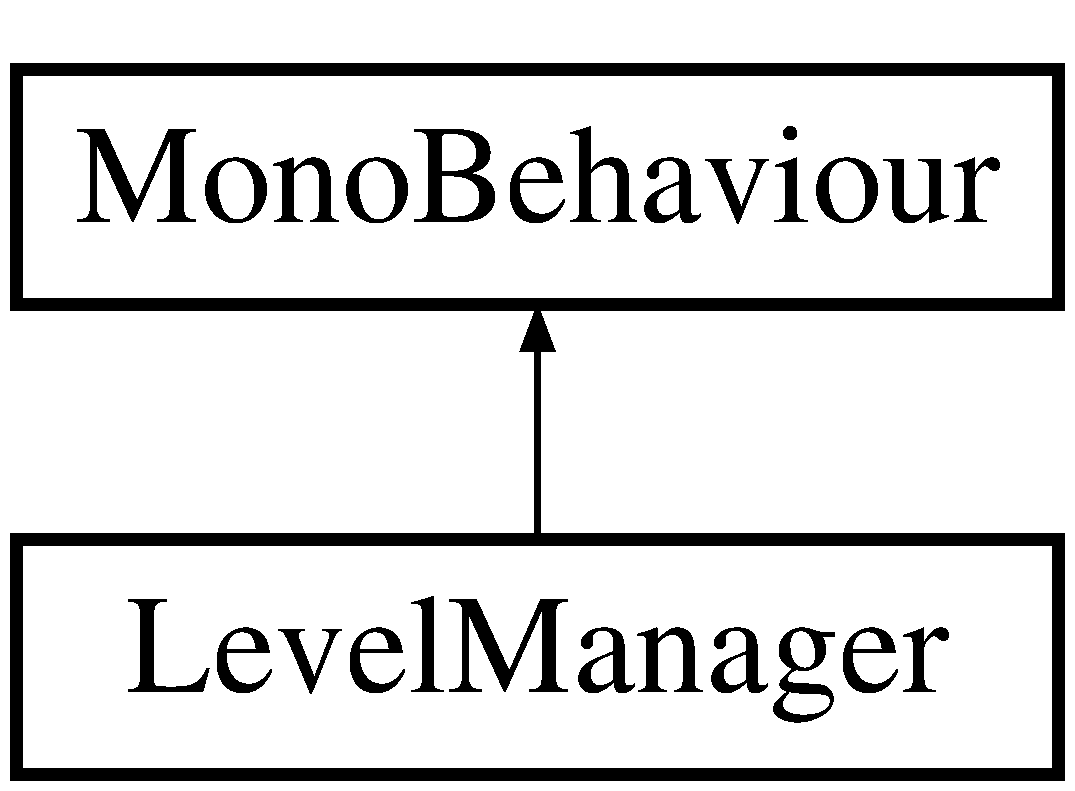
\includegraphics[height=2.000000cm]{class_level_manager}
\end{center}
\end{figure}
\subsection*{Metody publiczne}
\begin{DoxyCompactItemize}
\item 
void {\bf Awake} ()
\begin{DoxyCompactList}\small\item\em Ustawienie instancji klasy, do której można się później odwoływać w innych klasach. \end{DoxyCompactList}\item 
void {\bf Start} ()
\item 
void {\bf Update} ()
\begin{DoxyCompactList}\small\item\em Aktualizowanie pozycji gracza względem checkpointów, liczby punktów i upływu czasu od osiągnięcia ostatniego checkpointu. \end{DoxyCompactList}\item 
void {\bf Goto\+Next\+Level} (string level\+Name)
\begin{DoxyCompactList}\small\item\em Metoda uruchamiająca procedurę przejścia do następnego poziomu. \end{DoxyCompactList}\item 
void {\bf Kill\+Player} ()
\begin{DoxyCompactList}\small\item\em Uruchomienie procedury zabicia gracza. \end{DoxyCompactList}\end{DoxyCompactItemize}
\subsection*{Atrybuty publiczne}
\begin{DoxyCompactItemize}
\item 
{\bf Checkpoint} {\bf Debug\+Spawn}
\begin{DoxyCompactList}\small\item\em \doxyref{Checkpoint}{str.}{class_checkpoint} związany z spawnowaniem gracza w edytorze Unity (jeśli go ustawimy w Unity). \end{DoxyCompactList}\item 
int {\bf Bonus\+Cutoff\+Seconds}
\begin{DoxyCompactList}\small\item\em Czas na osiągnięcie nowego checkpointu. \end{DoxyCompactList}\item 
int {\bf Bonus\+Second\+Multiplier}
\begin{DoxyCompactList}\small\item\em Mnożnik dotyczący zdobotych punktów za dotarcie do checkpointu w wyznaczonym czasie. \end{DoxyCompactList}\end{DoxyCompactItemize}
\subsection*{Właściwości}
\begin{DoxyCompactItemize}
\item 
static {\bf Level\+Manager} {\bf Instance}\hspace{0.3cm}{\ttfamily  [get]}
\begin{DoxyCompactList}\small\item\em Instancja Level\+Managera. \end{DoxyCompactList}\item 
{\bf Player} {\bf Player}\hspace{0.3cm}{\ttfamily  [get]}
\begin{DoxyCompactList}\small\item\em Gracz. \end{DoxyCompactList}\item 
{\bf Camera\+Controller} {\bf Camera}\hspace{0.3cm}{\ttfamily  [get]}
\begin{DoxyCompactList}\small\item\em Kamera. \end{DoxyCompactList}\item 
Time\+Span {\bf Running\+Time}\hspace{0.3cm}{\ttfamily  [get]}
\begin{DoxyCompactList}\small\item\em Upływ czasu od ostatniej wartości \+\_\+started. \end{DoxyCompactList}\item 
int {\bf Current\+Time\+Bonus}\hspace{0.3cm}{\ttfamily  [get]}
\begin{DoxyCompactList}\small\item\em Obliczenie bonusu czasowego za osiągnięcie nowego checkpointu w wyznaczonym czasie. \end{DoxyCompactList}\end{DoxyCompactItemize}


\subsection{Dokumentacja funkcji składowych}
\index{Level\+Manager@{Level\+Manager}!Awake@{Awake}}
\index{Awake@{Awake}!Level\+Manager@{Level\+Manager}}
\subsubsection[{Awake()}]{\setlength{\rightskip}{0pt plus 5cm}void Level\+Manager.\+Awake (
\begin{DoxyParamCaption}
{}
\end{DoxyParamCaption}
)}\label{class_level_manager_a34758a17d38f61b86163674657c94256}


Ustawienie instancji klasy, do której można się później odwoływać w innych klasach. 

\index{Level\+Manager@{Level\+Manager}!Goto\+Next\+Level@{Goto\+Next\+Level}}
\index{Goto\+Next\+Level@{Goto\+Next\+Level}!Level\+Manager@{Level\+Manager}}
\subsubsection[{Goto\+Next\+Level(string level\+Name)}]{\setlength{\rightskip}{0pt plus 5cm}void Level\+Manager.\+Goto\+Next\+Level (
\begin{DoxyParamCaption}
\item[{string}]{level\+Name}
\end{DoxyParamCaption}
)}\label{class_level_manager_aff2b84fbe01a7639e716fa8eceae27b6}


Metoda uruchamiająca procedurę przejścia do następnego poziomu. 


\begin{DoxyParams}{Parametry}
{\em level\+Name} & \\
\hline
\end{DoxyParams}
\index{Level\+Manager@{Level\+Manager}!Kill\+Player@{Kill\+Player}}
\index{Kill\+Player@{Kill\+Player}!Level\+Manager@{Level\+Manager}}
\subsubsection[{Kill\+Player()}]{\setlength{\rightskip}{0pt plus 5cm}void Level\+Manager.\+Kill\+Player (
\begin{DoxyParamCaption}
{}
\end{DoxyParamCaption}
)}\label{class_level_manager_a8c82ee034d89e0f1b7cb732052393e5d}


Uruchomienie procedury zabicia gracza. 

\index{Level\+Manager@{Level\+Manager}!Start@{Start}}
\index{Start@{Start}!Level\+Manager@{Level\+Manager}}
\subsubsection[{Start()}]{\setlength{\rightskip}{0pt plus 5cm}void Level\+Manager.\+Start (
\begin{DoxyParamCaption}
{}
\end{DoxyParamCaption}
)}\label{class_level_manager_afcd5c1d3d30954925d73f22ec1d0ecce}




Posortowana lista checkpointów.

Jeśli nie ma checkpointów, ustaw flagę na -\/1, w przeciwnym wypadku ustaw indeks na 0.

Gracz i kamera są teraz w lokalnej pamięci podręcznej (cache) Level\+Managera.

Ustawienie wartości początkowej \+\_\+started na aktualny czas.

Przypisanie obiektów (gwiazdek) do poszczególnych checkpointów (patrząc wstecz od danego checkpointu).

Wykonywane tylko w edytorze Unity, ustawia domyślny punkt spawnu gracza jako Debug\+Spawn, jeśli ustawiony jest Debug\+Spawn (nie ma wartości null). \index{Level\+Manager@{Level\+Manager}!Update@{Update}}
\index{Update@{Update}!Level\+Manager@{Level\+Manager}}
\subsubsection[{Update()}]{\setlength{\rightskip}{0pt plus 5cm}void Level\+Manager.\+Update (
\begin{DoxyParamCaption}
{}
\end{DoxyParamCaption}
)}\label{class_level_manager_a874b53f003bb10ede09e45fc34da4db9}


Aktualizowanie pozycji gracza względem checkpointów, liczby punktów i upływu czasu od osiągnięcia ostatniego checkpointu. 

Sprawdzamy czy jesteśmy na ostatnim checkpoincie (jeśli tak, to nie ma sensu wykonywać dalszych operacji -\/ nie ma dalszych checkpointów).

Sprawdzamy czy osiągnęliśmy nowy checkpoint, jeśli nie, wracamy.

Kod wykonywany, gdy osiągnięto nowy checkpoint. Opuszczenie starego checkpointu.

Inkrementacja wartości indeksu obecnego checkpointu.

Wejście w nowy checkpoint.

Dodanie ewentualnego bonusu czasowego.

Zapisanie liczby punktów.

Zresetowanie czasu w \+\_\+started. 

\subsection{Dokumentacja atrybutów składowych}
\index{Level\+Manager@{Level\+Manager}!Bonus\+Cutoff\+Seconds@{Bonus\+Cutoff\+Seconds}}
\index{Bonus\+Cutoff\+Seconds@{Bonus\+Cutoff\+Seconds}!Level\+Manager@{Level\+Manager}}
\subsubsection[{Bonus\+Cutoff\+Seconds}]{\setlength{\rightskip}{0pt plus 5cm}int Level\+Manager.\+Bonus\+Cutoff\+Seconds}\label{class_level_manager_afa0d0d57f95ac84102937f8ed1b1f207}


Czas na osiągnięcie nowego checkpointu. 

\index{Level\+Manager@{Level\+Manager}!Bonus\+Second\+Multiplier@{Bonus\+Second\+Multiplier}}
\index{Bonus\+Second\+Multiplier@{Bonus\+Second\+Multiplier}!Level\+Manager@{Level\+Manager}}
\subsubsection[{Bonus\+Second\+Multiplier}]{\setlength{\rightskip}{0pt plus 5cm}int Level\+Manager.\+Bonus\+Second\+Multiplier}\label{class_level_manager_ab5817002a701639af6c54c4f1096e15c}


Mnożnik dotyczący zdobotych punktów za dotarcie do checkpointu w wyznaczonym czasie. 

\index{Level\+Manager@{Level\+Manager}!Debug\+Spawn@{Debug\+Spawn}}
\index{Debug\+Spawn@{Debug\+Spawn}!Level\+Manager@{Level\+Manager}}
\subsubsection[{Debug\+Spawn}]{\setlength{\rightskip}{0pt plus 5cm}{\bf Checkpoint} Level\+Manager.\+Debug\+Spawn}\label{class_level_manager_aad8098a740db596e926b6769e7946ce5}


\doxyref{Checkpoint}{str.}{class_checkpoint} związany z spawnowaniem gracza w edytorze Unity (jeśli go ustawimy w Unity). 



\subsection{Dokumentacja właściwości}
\index{Level\+Manager@{Level\+Manager}!Camera@{Camera}}
\index{Camera@{Camera}!Level\+Manager@{Level\+Manager}}
\subsubsection[{Camera}]{\setlength{\rightskip}{0pt plus 5cm}{\bf Camera\+Controller} Level\+Manager.\+Camera\hspace{0.3cm}{\ttfamily [get]}}\label{class_level_manager_a9eae24c0943ba6c66ad82d0809cfae03}


Kamera. 

\index{Level\+Manager@{Level\+Manager}!Current\+Time\+Bonus@{Current\+Time\+Bonus}}
\index{Current\+Time\+Bonus@{Current\+Time\+Bonus}!Level\+Manager@{Level\+Manager}}
\subsubsection[{Current\+Time\+Bonus}]{\setlength{\rightskip}{0pt plus 5cm}int Level\+Manager.\+Current\+Time\+Bonus\hspace{0.3cm}{\ttfamily [get]}}\label{class_level_manager_a5a916054e78f75f8aa1313d676d19c94}


Obliczenie bonusu czasowego za osiągnięcie nowego checkpointu w wyznaczonym czasie. 

\index{Level\+Manager@{Level\+Manager}!Instance@{Instance}}
\index{Instance@{Instance}!Level\+Manager@{Level\+Manager}}
\subsubsection[{Instance}]{\setlength{\rightskip}{0pt plus 5cm}{\bf Level\+Manager} Level\+Manager.\+Instance\hspace{0.3cm}{\ttfamily [static]}, {\ttfamily [get]}}\label{class_level_manager_a4e58c52b52fc7486c8f6ede86867be7b}


Instancja Level\+Managera. 

\index{Level\+Manager@{Level\+Manager}!Player@{Player}}
\index{Player@{Player}!Level\+Manager@{Level\+Manager}}
\subsubsection[{Player}]{\setlength{\rightskip}{0pt plus 5cm}{\bf Player} Level\+Manager.\+Player\hspace{0.3cm}{\ttfamily [get]}}\label{class_level_manager_a6a35055ac074557e9e209daea815fdc1}


Gracz. 

\index{Level\+Manager@{Level\+Manager}!Running\+Time@{Running\+Time}}
\index{Running\+Time@{Running\+Time}!Level\+Manager@{Level\+Manager}}
\subsubsection[{Running\+Time}]{\setlength{\rightskip}{0pt plus 5cm}Time\+Span Level\+Manager.\+Running\+Time\hspace{0.3cm}{\ttfamily [get]}}\label{class_level_manager_a71e1e09286757567577501bf1d5624ad}


Upływ czasu od ostatniej wartości \+\_\+started. 



Dokumentacja dla tej klasy została wygenerowana z pliku\+:\begin{DoxyCompactItemize}
\item 
C\+:/\+Users/\+Paul/\+Projects/\+Unity\+Game/\+Projekt/\+Assets/\+Code/Level\+Manager.\+cs\end{DoxyCompactItemize}

\section{Dokumentacja klasy Path\+Definition}
\label{class_path_definition}\index{Path\+Definition@{Path\+Definition}}


klasa \doxyref{Path\+Definition}{str.}{class_path_definition}  


Diagram dziedziczenia dla Path\+Definition\begin{figure}[H]
\begin{center}
\leavevmode
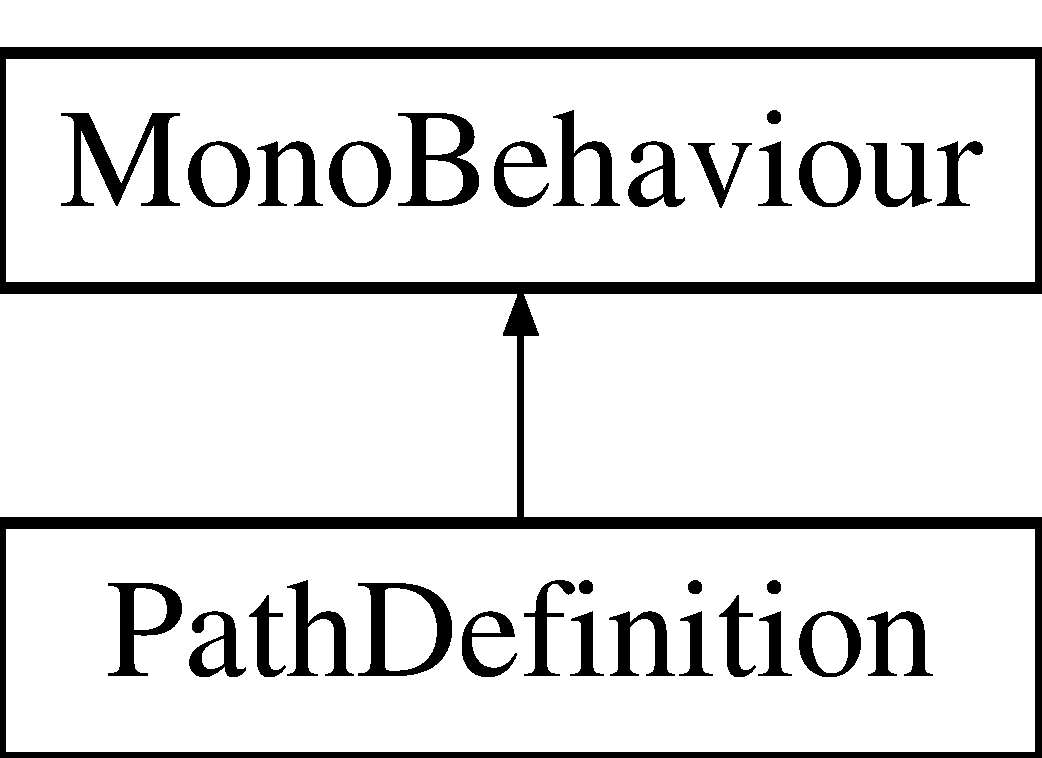
\includegraphics[height=2.000000cm]{class_path_definition}
\end{center}
\end{figure}
\subsection*{Metody publiczne}
\begin{DoxyCompactItemize}
\item 
I\+Enumerator$<$ Transform $>$ {\bf Get\+Path\+Enumerator} ()
\item 
void {\bf On\+Draw\+Gizmos} ()
\end{DoxyCompactItemize}
\subsection*{Atrybuty publiczne}
\begin{DoxyCompactItemize}
\item 
Transform[$\,$] {\bf Points}\label{class_path_definition_ab2d82757e323cdfcdb25cf2111c12310}

\begin{DoxyCompactList}\small\item\em Punkty sciezki. \end{DoxyCompactList}\end{DoxyCompactItemize}


\subsection{Opis szczegółowy}
klasa \doxyref{Path\+Definition}{str.}{class_path_definition} 



\subsection{Dokumentacja funkcji składowych}
\index{Path\+Definition@{Path\+Definition}!Get\+Path\+Enumerator@{Get\+Path\+Enumerator}}
\index{Get\+Path\+Enumerator@{Get\+Path\+Enumerator}!Path\+Definition@{Path\+Definition}}
\subsubsection[{Get\+Path\+Enumerator()}]{\setlength{\rightskip}{0pt plus 5cm}I\+Enumerator$<$Transform$>$ Path\+Definition.\+Get\+Path\+Enumerator (
\begin{DoxyParamCaption}
{}
\end{DoxyParamCaption}
)}\label{class_path_definition_a0526b4b4e15883dad98b64bbed920f96}
Enumerator punktow w sciezce. Zapewnia poruszanie sie np. platform w obie strony po sciezce. \index{Path\+Definition@{Path\+Definition}!On\+Draw\+Gizmos@{On\+Draw\+Gizmos}}
\index{On\+Draw\+Gizmos@{On\+Draw\+Gizmos}!Path\+Definition@{Path\+Definition}}
\subsubsection[{On\+Draw\+Gizmos()}]{\setlength{\rightskip}{0pt plus 5cm}void Path\+Definition.\+On\+Draw\+Gizmos (
\begin{DoxyParamCaption}
{}
\end{DoxyParamCaption}
)}\label{class_path_definition_a5539d857e10ad2827afc1fbce1512e47}
Rysowanie linii miedzy punktami sciezki w Scene view, upewniajac sie czy istnieje odpowiednia ilosc punktow i omijajac usuniete. 

Dokumentacja dla tej klasy została wygenerowana z pliku\+:\begin{DoxyCompactItemize}
\item 
C\+:/\+Users/\+Paul/\+Projects/\+Unity\+Game/\+Projekt/\+Assets/\+Code/Path\+Definition.\+cs\end{DoxyCompactItemize}

\section{Dokumentacja klasy Pathed\+Projectile}
\label{class_pathed_projectile}\index{Pathed\+Projectile@{Pathed\+Projectile}}
Diagram dziedziczenia dla Pathed\+Projectile\begin{figure}[H]
\begin{center}
\leavevmode
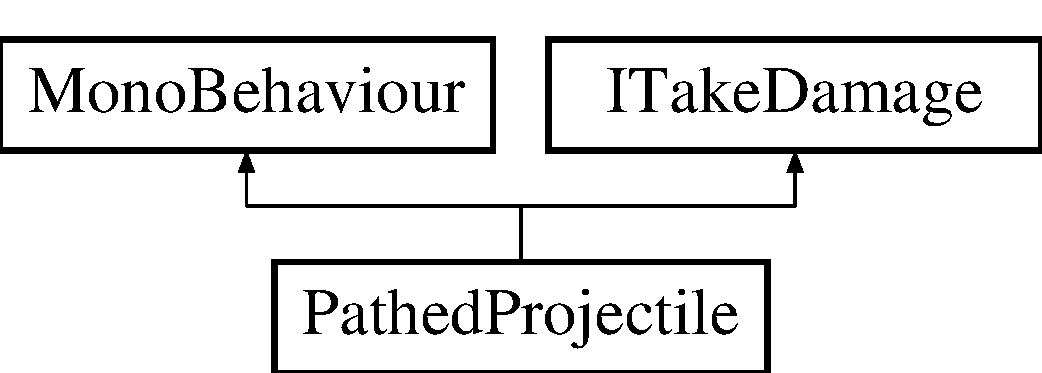
\includegraphics[height=2.000000cm]{class_pathed_projectile}
\end{center}
\end{figure}
\subsection*{Metody publiczne}
\begin{DoxyCompactItemize}
\item 
void {\bf Initialize} (Transform destination, float speed)
\begin{DoxyCompactList}\small\item\em Inicjalizacja celu i pr�dko�ci obiektu pocisku. \end{DoxyCompactList}\item 
void {\bf Update} ()
\begin{DoxyCompactList}\small\item\em Aktualizacja po�o�enia pocisku w czasie, oraz obs�uga jego zniszczenia. \end{DoxyCompactList}\item 
void {\bf Take\+Damage} (int damage, Game\+Object instigator)
\begin{DoxyCompactList}\small\item\em Metoda wywo�ywana po zestrzeleniu pocisku przez gracza. \end{DoxyCompactList}\end{DoxyCompactItemize}
\subsection*{Atrybuty publiczne}
\begin{DoxyCompactItemize}
\item 
Game\+Object {\bf Destroy\+Effect}
\begin{DoxyCompactList}\small\item\em Efekt towarzysz�cy zniszczeniu pocisku. \end{DoxyCompactList}\item 
int {\bf Points\+To\+Give\+Player}
\begin{DoxyCompactList}\small\item\em Punkty przyznawane graczowi za zestrzelenie pocisku. \end{DoxyCompactList}\item 
Audio\+Clip {\bf Destroy\+Sound}
\begin{DoxyCompactList}\small\item\em D�wi�k odtwarzany przy zniszczeniu pocisku. \end{DoxyCompactList}\end{DoxyCompactItemize}


\subsection{Dokumentacja funkcji składowych}
\index{Pathed\+Projectile@{Pathed\+Projectile}!Initialize@{Initialize}}
\index{Initialize@{Initialize}!Pathed\+Projectile@{Pathed\+Projectile}}
\subsubsection[{Initialize(\+Transform destination, float speed)}]{\setlength{\rightskip}{0pt plus 5cm}void Pathed\+Projectile.\+Initialize (
\begin{DoxyParamCaption}
\item[{Transform}]{destination, }
\item[{float}]{speed}
\end{DoxyParamCaption}
)}\label{class_pathed_projectile_a12dd7ed82badcadb184ac5a9430705b2}


Inicjalizacja celu i pr�dko�ci obiektu pocisku. 


\begin{DoxyParams}{Parametry}
{\em destination} & \\
\hline
{\em speed} & \\
\hline
\end{DoxyParams}
\index{Pathed\+Projectile@{Pathed\+Projectile}!Take\+Damage@{Take\+Damage}}
\index{Take\+Damage@{Take\+Damage}!Pathed\+Projectile@{Pathed\+Projectile}}
\subsubsection[{Take\+Damage(int damage, Game\+Object instigator)}]{\setlength{\rightskip}{0pt plus 5cm}void Pathed\+Projectile.\+Take\+Damage (
\begin{DoxyParamCaption}
\item[{int}]{damage, }
\item[{Game\+Object}]{instigator}
\end{DoxyParamCaption}
)}\label{class_pathed_projectile_a5caa718fce400e03378fe8a999daeadc}


Metoda wywo�ywana po zestrzeleniu pocisku przez gracza. 


\begin{DoxyParams}{Parametry}
{\em damage} & \\
\hline
{\em instigator} & \\
\hline
\end{DoxyParams}
Uruchomienie efektu zniszczenia pocisku.

Zniszczenie obiektu pocisku.

Przyznanie punkt�w graczowi za zestrzelenie pocisku. 

Implementuje {\bf I\+Take\+Damage} \doxyref{}{str.}{interface_i_take_damage}.

\index{Pathed\+Projectile@{Pathed\+Projectile}!Update@{Update}}
\index{Update@{Update}!Pathed\+Projectile@{Pathed\+Projectile}}
\subsubsection[{Update()}]{\setlength{\rightskip}{0pt plus 5cm}void Pathed\+Projectile.\+Update (
\begin{DoxyParamCaption}
{}
\end{DoxyParamCaption}
)}\label{class_pathed_projectile_a51f8264c920fcd82f4d48ea703f88009}


Aktualizacja po�o�enia pocisku w czasie, oraz obs�uga jego zniszczenia. 

Aktualizacja po�o�enia pocisku w czasie.

Sprawdzenie czy pocisk dotar� do celu.

Uruchomienie efektu zniszczenia pocisku.

Odtworzenie d�wi�ku zniszczenia pocisku.

Zniszczenie obiektu pocisku, je�li dotar� do celu. 

\subsection{Dokumentacja atrybutów składowych}
\index{Pathed\+Projectile@{Pathed\+Projectile}!Destroy\+Effect@{Destroy\+Effect}}
\index{Destroy\+Effect@{Destroy\+Effect}!Pathed\+Projectile@{Pathed\+Projectile}}
\subsubsection[{Destroy\+Effect}]{\setlength{\rightskip}{0pt plus 5cm}Game\+Object Pathed\+Projectile.\+Destroy\+Effect}\label{class_pathed_projectile_a332f3a849d5d592e3ecc52c52bbac326}


Efekt towarzysz�cy zniszczeniu pocisku. 

\index{Pathed\+Projectile@{Pathed\+Projectile}!Destroy\+Sound@{Destroy\+Sound}}
\index{Destroy\+Sound@{Destroy\+Sound}!Pathed\+Projectile@{Pathed\+Projectile}}
\subsubsection[{Destroy\+Sound}]{\setlength{\rightskip}{0pt plus 5cm}Audio\+Clip Pathed\+Projectile.\+Destroy\+Sound}\label{class_pathed_projectile_ab069aa20f20da80567b061e68330b4d3}


D�wi�k odtwarzany przy zniszczeniu pocisku. 

\index{Pathed\+Projectile@{Pathed\+Projectile}!Points\+To\+Give\+Player@{Points\+To\+Give\+Player}}
\index{Points\+To\+Give\+Player@{Points\+To\+Give\+Player}!Pathed\+Projectile@{Pathed\+Projectile}}
\subsubsection[{Points\+To\+Give\+Player}]{\setlength{\rightskip}{0pt plus 5cm}int Pathed\+Projectile.\+Points\+To\+Give\+Player}\label{class_pathed_projectile_ab88d75f6caac96633c158f9c275ab3dc}


Punkty przyznawane graczowi za zestrzelenie pocisku. 



Dokumentacja dla tej klasy została wygenerowana z pliku\+:\begin{DoxyCompactItemize}
\item 
C\+:/\+Users/\+Paul/\+Projects/\+Unity\+Game/\+Projekt/\+Assets/\+Code/Pathed\+Projectile.\+cs\end{DoxyCompactItemize}

\section{Dokumentacja klasy Pathed\+Projectile\+Spawner}
\label{class_pathed_projectile_spawner}\index{Pathed\+Projectile\+Spawner@{Pathed\+Projectile\+Spawner}}


Tworzenie pocisku poruszającego się po danej ścieżce.  


Diagram dziedziczenia dla Pathed\+Projectile\+Spawner\begin{figure}[H]
\begin{center}
\leavevmode
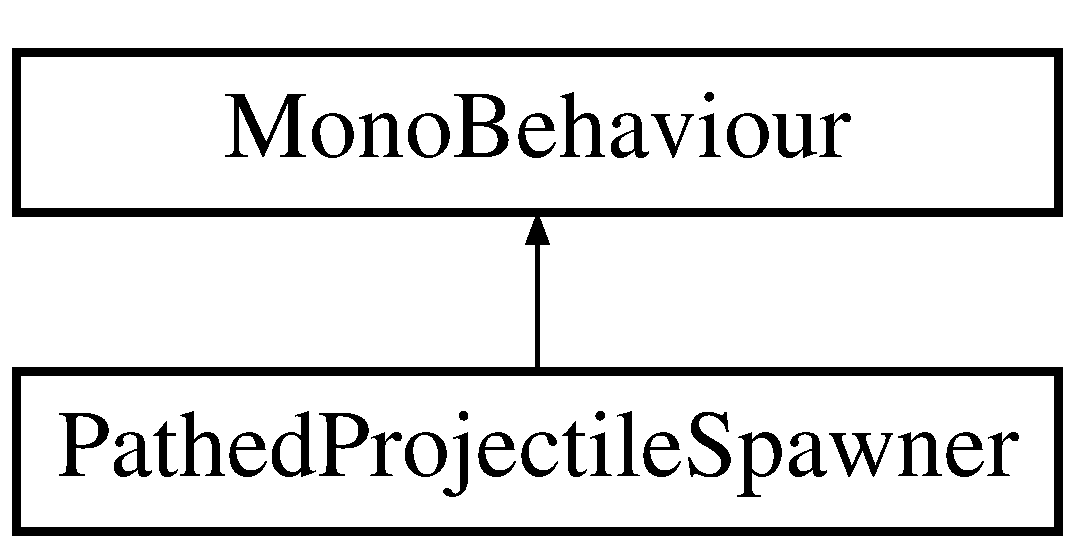
\includegraphics[height=2.000000cm]{class_pathed_projectile_spawner}
\end{center}
\end{figure}
\subsection*{Metody publiczne}
\begin{DoxyCompactItemize}
\item 
void {\bf Start} ()
\begin{DoxyCompactList}\small\item\em Ustawienie początkowej wartości czasu kolejnego wystrzału na częstotliwość oddawania strzałów. \end{DoxyCompactList}\item 
void {\bf Update} ()
\begin{DoxyCompactList}\small\item\em Metoda odmierzająca czas do kolejnego wystrzału, inicjująca obiekt pocisku w danym położeniu, o danej prędkości i wyznaczonym celu. Odpowiada również za inicjowanie efektu stworzenia pocisku w świecie gry oraz odtworzenie dźwięku. \end{DoxyCompactList}\item 
void {\bf On\+Draw\+Gizmos} ()
\begin{DoxyCompactList}\small\item\em Tworzenie czerwonej linii w widoku Scene podczas wystrzału, od jego źródła do celu. \end{DoxyCompactList}\end{DoxyCompactItemize}
\subsection*{Atrybuty publiczne}
\begin{DoxyCompactItemize}
\item 
Transform {\bf Destination}
\begin{DoxyCompactList}\small\item\em Cel. \end{DoxyCompactList}\item 
{\bf Pathed\+Projectile} {\bf Projectile}
\begin{DoxyCompactList}\small\item\em Obiekt pocisku. \end{DoxyCompactList}\item 
Game\+Object {\bfseries Spawn\+Effect}\label{class_pathed_projectile_spawner_a05f0c6114aeb62a7f208757f3bb669b0}

\item 
float {\bf Speed}
\begin{DoxyCompactList}\small\item\em Prędkość pocisku. \end{DoxyCompactList}\item 
float {\bf Fire\+Rate}
\begin{DoxyCompactList}\small\item\em Częstotliwość oddawania strzałów. \end{DoxyCompactList}\item 
Audio\+Clip {\bf Spawn\+Projectile\+Sound}
\begin{DoxyCompactList}\small\item\em Dźwięk odtwarzany podczas wystrzału pocisku. \end{DoxyCompactList}\item 
Animator {\bf Animator}
\begin{DoxyCompactList}\small\item\em Obiekt animacji potrzebny do ustawienia efektu przejścia. \end{DoxyCompactList}\end{DoxyCompactItemize}


\subsection{Opis szczegółowy}
Tworzenie pocisku poruszającego się po danej ścieżce. 



\subsection{Dokumentacja funkcji składowych}
\index{Pathed\+Projectile\+Spawner@{Pathed\+Projectile\+Spawner}!On\+Draw\+Gizmos@{On\+Draw\+Gizmos}}
\index{On\+Draw\+Gizmos@{On\+Draw\+Gizmos}!Pathed\+Projectile\+Spawner@{Pathed\+Projectile\+Spawner}}
\subsubsection[{On\+Draw\+Gizmos()}]{\setlength{\rightskip}{0pt plus 5cm}void Pathed\+Projectile\+Spawner.\+On\+Draw\+Gizmos (
\begin{DoxyParamCaption}
{}
\end{DoxyParamCaption}
)}\label{class_pathed_projectile_spawner_a88ebe3827d4ec865088ed3b33b04da2a}


Tworzenie czerwonej linii w widoku Scene podczas wystrzału, od jego źródła do celu. 

\index{Pathed\+Projectile\+Spawner@{Pathed\+Projectile\+Spawner}!Start@{Start}}
\index{Start@{Start}!Pathed\+Projectile\+Spawner@{Pathed\+Projectile\+Spawner}}
\subsubsection[{Start()}]{\setlength{\rightskip}{0pt plus 5cm}void Pathed\+Projectile\+Spawner.\+Start (
\begin{DoxyParamCaption}
{}
\end{DoxyParamCaption}
)}\label{class_pathed_projectile_spawner_abc587266a7eed7f8acfab4f941ba1a9b}


Ustawienie początkowej wartości czasu kolejnego wystrzału na częstotliwość oddawania strzałów. 

\index{Pathed\+Projectile\+Spawner@{Pathed\+Projectile\+Spawner}!Update@{Update}}
\index{Update@{Update}!Pathed\+Projectile\+Spawner@{Pathed\+Projectile\+Spawner}}
\subsubsection[{Update()}]{\setlength{\rightskip}{0pt plus 5cm}void Pathed\+Projectile\+Spawner.\+Update (
\begin{DoxyParamCaption}
{}
\end{DoxyParamCaption}
)}\label{class_pathed_projectile_spawner_abc7aedd014236174fc8fd43359e352de}


Metoda odmierzająca czas do kolejnego wystrzału, inicjująca obiekt pocisku w danym położeniu, o danej prędkości i wyznaczonym celu. Odpowiada również za inicjowanie efektu stworzenia pocisku w świecie gry oraz odtworzenie dźwięku. 



\subsection{Dokumentacja atrybutów składowych}
\index{Pathed\+Projectile\+Spawner@{Pathed\+Projectile\+Spawner}!Animator@{Animator}}
\index{Animator@{Animator}!Pathed\+Projectile\+Spawner@{Pathed\+Projectile\+Spawner}}
\subsubsection[{Animator}]{\setlength{\rightskip}{0pt plus 5cm}Animator Pathed\+Projectile\+Spawner.\+Animator}\label{class_pathed_projectile_spawner_a3edee672c39ada316ed3ec99686a8b42}


Obiekt animacji potrzebny do ustawienia efektu przejścia. 

\index{Pathed\+Projectile\+Spawner@{Pathed\+Projectile\+Spawner}!Destination@{Destination}}
\index{Destination@{Destination}!Pathed\+Projectile\+Spawner@{Pathed\+Projectile\+Spawner}}
\subsubsection[{Destination}]{\setlength{\rightskip}{0pt plus 5cm}Transform Pathed\+Projectile\+Spawner.\+Destination}\label{class_pathed_projectile_spawner_a641d2522461c18b7e38ca57c0725755b}


Cel. 

\index{Pathed\+Projectile\+Spawner@{Pathed\+Projectile\+Spawner}!Fire\+Rate@{Fire\+Rate}}
\index{Fire\+Rate@{Fire\+Rate}!Pathed\+Projectile\+Spawner@{Pathed\+Projectile\+Spawner}}
\subsubsection[{Fire\+Rate}]{\setlength{\rightskip}{0pt plus 5cm}float Pathed\+Projectile\+Spawner.\+Fire\+Rate}\label{class_pathed_projectile_spawner_a77143c5d27e069a0338a150eca991f27}


Częstotliwość oddawania strzałów. 

\index{Pathed\+Projectile\+Spawner@{Pathed\+Projectile\+Spawner}!Projectile@{Projectile}}
\index{Projectile@{Projectile}!Pathed\+Projectile\+Spawner@{Pathed\+Projectile\+Spawner}}
\subsubsection[{Projectile}]{\setlength{\rightskip}{0pt plus 5cm}{\bf Pathed\+Projectile} Pathed\+Projectile\+Spawner.\+Projectile}\label{class_pathed_projectile_spawner_a8b72edf1a8fd037b4ef989c3a061be51}


Obiekt pocisku. 

\index{Pathed\+Projectile\+Spawner@{Pathed\+Projectile\+Spawner}!Spawn\+Projectile\+Sound@{Spawn\+Projectile\+Sound}}
\index{Spawn\+Projectile\+Sound@{Spawn\+Projectile\+Sound}!Pathed\+Projectile\+Spawner@{Pathed\+Projectile\+Spawner}}
\subsubsection[{Spawn\+Projectile\+Sound}]{\setlength{\rightskip}{0pt plus 5cm}Audio\+Clip Pathed\+Projectile\+Spawner.\+Spawn\+Projectile\+Sound}\label{class_pathed_projectile_spawner_ab653acbecff474b6e0f58db623b1acea}


Dźwięk odtwarzany podczas wystrzału pocisku. 

\index{Pathed\+Projectile\+Spawner@{Pathed\+Projectile\+Spawner}!Speed@{Speed}}
\index{Speed@{Speed}!Pathed\+Projectile\+Spawner@{Pathed\+Projectile\+Spawner}}
\subsubsection[{Speed}]{\setlength{\rightskip}{0pt plus 5cm}float Pathed\+Projectile\+Spawner.\+Speed}\label{class_pathed_projectile_spawner_a03c624ef3218b0cc67b1a6c68479339d}


Prędkość pocisku. 



Dokumentacja dla tej klasy została wygenerowana z pliku\+:\begin{DoxyCompactItemize}
\item 
C\+:/\+Users/\+Paul/\+Projects/\+Unity\+Game/\+Projekt/\+Assets/\+Code/Pathed\+Projectile\+Spawner.\+cs\end{DoxyCompactItemize}

\section{Dokumentacja klasy Player}
\label{class_player}\index{Player@{Player}}


klasa \doxyref{Player}{str.}{class_player}  


Diagram dziedziczenia dla Player\begin{figure}[H]
\begin{center}
\leavevmode
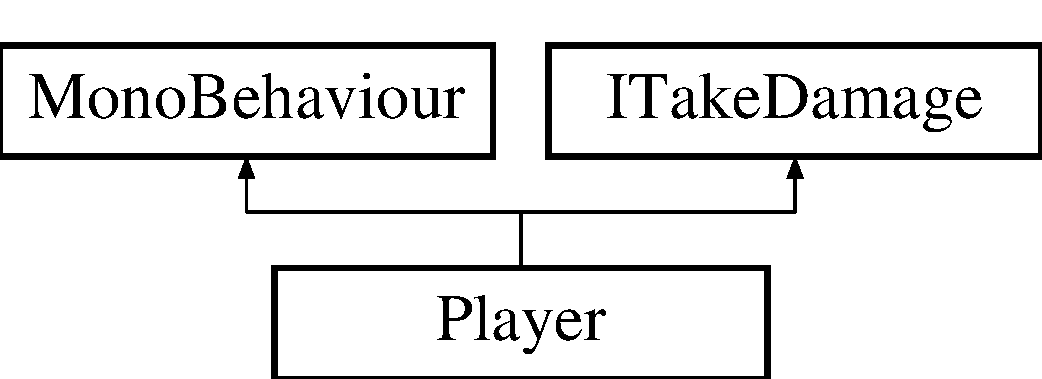
\includegraphics[height=2.000000cm]{class_player}
\end{center}
\end{figure}
\subsection*{Metody publiczne}
\begin{DoxyCompactItemize}
\item 
void {\bf Awake} ()
\begin{DoxyCompactList}\small\item\em Ustawianie początkowych ustawień gracza. \end{DoxyCompactList}\item 
void {\bf Update} ()
\begin{DoxyCompactList}\small\item\em Wywolywane dla kazdej klatki animacji gry. Wywolanie metody Handle\+Imput(), obslugujacej nacisniecie klawiszy przez gracza. Ustawiana jest predkosc w poziomie, zalezna od kierunku zwrotu gracza, oraz tego czy znajduje sie w powietrzu lub na ziemi. \end{DoxyCompactList}\item 
void {\bf Finish\+Level} ()
\begin{DoxyCompactList}\small\item\em Metoda uruchamiana po przejściu danego poziomu gry. Deaktywuje ona Box\+Collider2\+D i ruch gracza. \end{DoxyCompactList}\item 
void {\bf Kill} ()
\begin{DoxyCompactList}\small\item\em Zresetowanie ustawień gracza po śmierci. \end{DoxyCompactList}\item 
void {\bf Respawn\+At} (Transform spawn\+Point)
\begin{DoxyCompactList}\small\item\em Respawnowanie gracza w danym punkcie i zmiana jego ustawień początkowych. \end{DoxyCompactList}\item 
void {\bf Take\+Damage} (int damage, Game\+Object instagator)
\begin{DoxyCompactList}\small\item\em Inicjowanie efektu obrażeń gracza (czerwona chmura cząsteczek) oraz zmniejszenie punktów zdrowia gracza po zadanych obrażeniach, prowadzące ewentualnie do jego śmierci. \end{DoxyCompactList}\item 
void {\bf Give\+Health} (int health, Game\+Object instagator)
\begin{DoxyCompactList}\small\item\em Dodanie punktów zdrowia po zebraniu apteczki. \end{DoxyCompactList}\item 
void {\bf Handle\+Input} ()
\begin{DoxyCompactList}\small\item\em Obsluga interakcji gracza (nacisniecia klawisza A lub D), umozliwiajaca obrot. Nacisniecie spacji wykonuje skok. \end{DoxyCompactList}\end{DoxyCompactItemize}
\subsection*{Atrybuty publiczne}
\begin{DoxyCompactItemize}
\item 
float {\bf Max\+Speed} = 8
\begin{DoxyCompactList}\small\item\em Maksymalna liczba jednostek na sekunde, jakie gracz moze przejsc. \end{DoxyCompactList}\item 
float {\bf Speed\+Acceleration\+On\+Ground} = 10f
\begin{DoxyCompactList}\small\item\em Jak szybko moze zmienic sie predkosc gracza na ziemi. \end{DoxyCompactList}\item 
float {\bf Speed\+Acceleration\+In\+Air} = 5f
\begin{DoxyCompactList}\small\item\em Jak szybko moze zmienic sie predkosc gracza w powietrzu \end{DoxyCompactList}\item 
int {\bf Max\+Health} = 100
\begin{DoxyCompactList}\small\item\em Maksymalna wartość punktów zdrowia. \end{DoxyCompactList}\item 
Game\+Object {\bf Ouch\+Effect}
\begin{DoxyCompactList}\small\item\em Efekt wyzwalany podczas otrzymania obrażeń. \end{DoxyCompactList}\item 
{\bf Projectile} {\bf Projectile}
\begin{DoxyCompactList}\small\item\em Piła \end{DoxyCompactList}\item 
float {\bf Fire\+Rate}
\begin{DoxyCompactList}\small\item\em Częstotliwość z którą strzela \end{DoxyCompactList}\item 
Transform {\bf Projectile\+Fire\+Location}
\begin{DoxyCompactList}\small\item\em Lokalizacja Piły. \end{DoxyCompactList}\item 
Game\+Object {\bf Fire\+Projectile\+Effect}
\begin{DoxyCompactList}\small\item\em Fire projectile effect. \end{DoxyCompactList}\item 
Audio\+Clip {\bf Player\+Hit\+Sound}
\begin{DoxyCompactList}\small\item\em Dźwięk odtwarzany po trafieniu gracza przez wroga. \end{DoxyCompactList}\item 
Audio\+Clip {\bf Player\+Shoot\+Sound}
\begin{DoxyCompactList}\small\item\em Dźwięk odtwarzany po wystrzeleniu pocisku przez gracza. \end{DoxyCompactList}\item 
Audio\+Clip {\bf Player\+Health\+Sound}
\begin{DoxyCompactList}\small\item\em Dźwięk odtwarzany po zebraniu apteczki przez gracza. \end{DoxyCompactList}\item 
Animator {\bfseries Animator}\label{class_player_a5409bcd7ffe8235f1388fa5a895e041d}

\end{DoxyCompactItemize}
\subsection*{Właściwości}
\begin{DoxyCompactItemize}
\item 
int {\bf Health}\hspace{0.3cm}{\ttfamily  [get]}
\begin{DoxyCompactList}\small\item\em Wartośc punktów zdrowia. \end{DoxyCompactList}\item 
bool {\bf Is\+Dead}\hspace{0.3cm}{\ttfamily  [get]}
\begin{DoxyCompactList}\small\item\em Zmienna bool służąca do zapamiętania informacji o śmierci gracza. \end{DoxyCompactList}\end{DoxyCompactItemize}


\subsection{Opis szczegółowy}
klasa \doxyref{Player}{str.}{class_player} 



\subsection{Dokumentacja funkcji składowych}
\index{Player@{Player}!Awake@{Awake}}
\index{Awake@{Awake}!Player@{Player}}
\subsubsection[{Awake()}]{\setlength{\rightskip}{0pt plus 5cm}void Player.\+Awake (
\begin{DoxyParamCaption}
{}
\end{DoxyParamCaption}
)}\label{class_player_aaddfa9f3b558df64f5d1d09e2b906901}


Ustawianie początkowych ustawień gracza. 

Jesli gracz jest obrocony, wartosc local\+Scale.\+x bedzie mniejsza od 0.

Punkty zdrowia mają wartość maksymalną. \index{Player@{Player}!Finish\+Level@{Finish\+Level}}
\index{Finish\+Level@{Finish\+Level}!Player@{Player}}
\subsubsection[{Finish\+Level()}]{\setlength{\rightskip}{0pt plus 5cm}void Player.\+Finish\+Level (
\begin{DoxyParamCaption}
{}
\end{DoxyParamCaption}
)}\label{class_player_a91d819ca123465f0c47f17f2179fd391}


Metoda uruchamiana po przejściu danego poziomu gry. Deaktywuje ona Box\+Collider2\+D i ruch gracza. 

\index{Player@{Player}!Give\+Health@{Give\+Health}}
\index{Give\+Health@{Give\+Health}!Player@{Player}}
\subsubsection[{Give\+Health(int health, Game\+Object instagator)}]{\setlength{\rightskip}{0pt plus 5cm}void Player.\+Give\+Health (
\begin{DoxyParamCaption}
\item[{int}]{health, }
\item[{Game\+Object}]{instagator}
\end{DoxyParamCaption}
)}\label{class_player_ab5b7362150ceb3bdd0ea0264799a1b60}


Dodanie punktów zdrowia po zebraniu apteczki. 


\begin{DoxyParams}{Parametry}
{\em health} & \\
\hline
{\em instagator} & \\
\hline
\end{DoxyParams}
Health += Mathf.\+Min(Health + health, Max\+Health); \index{Player@{Player}!Handle\+Input@{Handle\+Input}}
\index{Handle\+Input@{Handle\+Input}!Player@{Player}}
\subsubsection[{Handle\+Input()}]{\setlength{\rightskip}{0pt plus 5cm}void Player.\+Handle\+Input (
\begin{DoxyParamCaption}
{}
\end{DoxyParamCaption}
)}\label{class_player_a6d893d1229110e7eb17eb7d895198717}


Obsluga interakcji gracza (nacisniecia klawisza A lub D), umozliwiajaca obrot. Nacisniecie spacji wykonuje skok. 

\index{Player@{Player}!Kill@{Kill}}
\index{Kill@{Kill}!Player@{Player}}
\subsubsection[{Kill()}]{\setlength{\rightskip}{0pt plus 5cm}void Player.\+Kill (
\begin{DoxyParamCaption}
{}
\end{DoxyParamCaption}
)}\label{class_player_aad95a8298c4f1d4b8ae695c92ef42c92}


Zresetowanie ustawień gracza po śmierci. 

Gracz lekko podskakuje pionowo po śmierci. \index{Player@{Player}!Respawn\+At@{Respawn\+At}}
\index{Respawn\+At@{Respawn\+At}!Player@{Player}}
\subsubsection[{Respawn\+At(\+Transform spawn\+Point)}]{\setlength{\rightskip}{0pt plus 5cm}void Player.\+Respawn\+At (
\begin{DoxyParamCaption}
\item[{Transform}]{spawn\+Point}
\end{DoxyParamCaption}
)}\label{class_player_a79731bebcf341b5785d28751b737975d}


Respawnowanie gracza w danym punkcie i zmiana jego ustawień początkowych. 


\begin{DoxyParams}{Parametry}
{\em spawn\+Point} & \\
\hline
\end{DoxyParams}
\index{Player@{Player}!Take\+Damage@{Take\+Damage}}
\index{Take\+Damage@{Take\+Damage}!Player@{Player}}
\subsubsection[{Take\+Damage(int damage, Game\+Object instagator)}]{\setlength{\rightskip}{0pt plus 5cm}void Player.\+Take\+Damage (
\begin{DoxyParamCaption}
\item[{int}]{damage, }
\item[{Game\+Object}]{instagator}
\end{DoxyParamCaption}
)}\label{class_player_ad85aa8e7e4501b49f9d20c4eff6c98a2}


Inicjowanie efektu obrażeń gracza (czerwona chmura cząsteczek) oraz zmniejszenie punktów zdrowia gracza po zadanych obrażeniach, prowadzące ewentualnie do jego śmierci. 


\begin{DoxyParams}{Parametry}
{\em damage} & \\
\hline
\end{DoxyParams}


Implementuje {\bf I\+Take\+Damage} \doxyref{}{str.}{interface_i_take_damage}.

\index{Player@{Player}!Update@{Update}}
\index{Update@{Update}!Player@{Player}}
\subsubsection[{Update()}]{\setlength{\rightskip}{0pt plus 5cm}void Player.\+Update (
\begin{DoxyParamCaption}
{}
\end{DoxyParamCaption}
)}\label{class_player_aace80372e18e32fe177e295fe5d93ba8}


Wywolywane dla kazdej klatki animacji gry. Wywolanie metody Handle\+Imput(), obslugujacej nacisniecie klawiszy przez gracza. Ustawiana jest predkosc w poziomie, zalezna od kierunku zwrotu gracza, oraz tego czy znajduje sie w powietrzu lub na ziemi. 

Aktualizacja czasu przeładowywania broni.

Ustawienie wartości prędkości jako liczby między 0, a 1. 

\subsection{Dokumentacja atrybutów składowych}
\index{Player@{Player}!Fire\+Projectile\+Effect@{Fire\+Projectile\+Effect}}
\index{Fire\+Projectile\+Effect@{Fire\+Projectile\+Effect}!Player@{Player}}
\subsubsection[{Fire\+Projectile\+Effect}]{\setlength{\rightskip}{0pt plus 5cm}Game\+Object Player.\+Fire\+Projectile\+Effect}\label{class_player_a6ec4f072105738364ede9225cc52c535}


Fire projectile effect. 

\index{Player@{Player}!Fire\+Rate@{Fire\+Rate}}
\index{Fire\+Rate@{Fire\+Rate}!Player@{Player}}
\subsubsection[{Fire\+Rate}]{\setlength{\rightskip}{0pt plus 5cm}float Player.\+Fire\+Rate}\label{class_player_a78d79a824776d573853f7047ba972e11}


Częstotliwość z którą strzela 

\index{Player@{Player}!Max\+Health@{Max\+Health}}
\index{Max\+Health@{Max\+Health}!Player@{Player}}
\subsubsection[{Max\+Health}]{\setlength{\rightskip}{0pt plus 5cm}int Player.\+Max\+Health = 100}\label{class_player_aa31df936a1c5641ed287c77c755eb433}


Maksymalna wartość punktów zdrowia. 

\index{Player@{Player}!Max\+Speed@{Max\+Speed}}
\index{Max\+Speed@{Max\+Speed}!Player@{Player}}
\subsubsection[{Max\+Speed}]{\setlength{\rightskip}{0pt plus 5cm}float Player.\+Max\+Speed = 8}\label{class_player_a00cb3f26349dd5f58ad0a6135b763a07}


Maksymalna liczba jednostek na sekunde, jakie gracz moze przejsc. 

\index{Player@{Player}!Ouch\+Effect@{Ouch\+Effect}}
\index{Ouch\+Effect@{Ouch\+Effect}!Player@{Player}}
\subsubsection[{Ouch\+Effect}]{\setlength{\rightskip}{0pt plus 5cm}Game\+Object Player.\+Ouch\+Effect}\label{class_player_ab4991d947bebe270dbf98a6de3007926}


Efekt wyzwalany podczas otrzymania obrażeń. 

\index{Player@{Player}!Player\+Health\+Sound@{Player\+Health\+Sound}}
\index{Player\+Health\+Sound@{Player\+Health\+Sound}!Player@{Player}}
\subsubsection[{Player\+Health\+Sound}]{\setlength{\rightskip}{0pt plus 5cm}Audio\+Clip Player.\+Player\+Health\+Sound}\label{class_player_a3374795dc2e83ba343d48f2023367c22}


Dźwięk odtwarzany po zebraniu apteczki przez gracza. 

\index{Player@{Player}!Player\+Hit\+Sound@{Player\+Hit\+Sound}}
\index{Player\+Hit\+Sound@{Player\+Hit\+Sound}!Player@{Player}}
\subsubsection[{Player\+Hit\+Sound}]{\setlength{\rightskip}{0pt plus 5cm}Audio\+Clip Player.\+Player\+Hit\+Sound}\label{class_player_a1274016f3c8907410af60aba1033b258}


Dźwięk odtwarzany po trafieniu gracza przez wroga. 

\index{Player@{Player}!Player\+Shoot\+Sound@{Player\+Shoot\+Sound}}
\index{Player\+Shoot\+Sound@{Player\+Shoot\+Sound}!Player@{Player}}
\subsubsection[{Player\+Shoot\+Sound}]{\setlength{\rightskip}{0pt plus 5cm}Audio\+Clip Player.\+Player\+Shoot\+Sound}\label{class_player_ab0fa5ed275c214cddd36a228d47695af}


Dźwięk odtwarzany po wystrzeleniu pocisku przez gracza. 

\index{Player@{Player}!Projectile@{Projectile}}
\index{Projectile@{Projectile}!Player@{Player}}
\subsubsection[{Projectile}]{\setlength{\rightskip}{0pt plus 5cm}{\bf Projectile} Player.\+Projectile}\label{class_player_ad8a413d5f8b8e7b585f5e61763de7f89}


Piła 

\index{Player@{Player}!Projectile\+Fire\+Location@{Projectile\+Fire\+Location}}
\index{Projectile\+Fire\+Location@{Projectile\+Fire\+Location}!Player@{Player}}
\subsubsection[{Projectile\+Fire\+Location}]{\setlength{\rightskip}{0pt plus 5cm}Transform Player.\+Projectile\+Fire\+Location}\label{class_player_aa256ec66d5f9405a331360eccbfa6299}


Lokalizacja Piły. 

\index{Player@{Player}!Speed\+Acceleration\+In\+Air@{Speed\+Acceleration\+In\+Air}}
\index{Speed\+Acceleration\+In\+Air@{Speed\+Acceleration\+In\+Air}!Player@{Player}}
\subsubsection[{Speed\+Acceleration\+In\+Air}]{\setlength{\rightskip}{0pt plus 5cm}float Player.\+Speed\+Acceleration\+In\+Air = 5f}\label{class_player_a6a71edc877a84d4f038fcc2b8e4f2843}


Jak szybko moze zmienic sie predkosc gracza w powietrzu 

\index{Player@{Player}!Speed\+Acceleration\+On\+Ground@{Speed\+Acceleration\+On\+Ground}}
\index{Speed\+Acceleration\+On\+Ground@{Speed\+Acceleration\+On\+Ground}!Player@{Player}}
\subsubsection[{Speed\+Acceleration\+On\+Ground}]{\setlength{\rightskip}{0pt plus 5cm}float Player.\+Speed\+Acceleration\+On\+Ground = 10f}\label{class_player_ae1d47d3f4f67909f7498d900c1feedfa}


Jak szybko moze zmienic sie predkosc gracza na ziemi. 



\subsection{Dokumentacja właściwości}
\index{Player@{Player}!Health@{Health}}
\index{Health@{Health}!Player@{Player}}
\subsubsection[{Health}]{\setlength{\rightskip}{0pt plus 5cm}int Player.\+Health\hspace{0.3cm}{\ttfamily [get]}}\label{class_player_a129d77184feb05c2743ef38726dc23da}


Wartośc punktów zdrowia. 

\index{Player@{Player}!Is\+Dead@{Is\+Dead}}
\index{Is\+Dead@{Is\+Dead}!Player@{Player}}
\subsubsection[{Is\+Dead}]{\setlength{\rightskip}{0pt plus 5cm}bool Player.\+Is\+Dead\hspace{0.3cm}{\ttfamily [get]}}\label{class_player_a7d0c0007bf91eb3eb887b7ab08f49cd3}


Zmienna bool służąca do zapamiętania informacji o śmierci gracza. 



Dokumentacja dla tej klasy została wygenerowana z pliku\+:\begin{DoxyCompactItemize}
\item 
C\+:/\+Users/\+Paul/\+Projects/\+Unity\+Game/\+Projekt/\+Assets/\+Code/Player.\+cs\end{DoxyCompactItemize}

\section{Dokumentacja klasy Player\+Bounds}
\label{class_player_bounds}\index{Player\+Bounds@{Player\+Bounds}}


Klasa ograniczająca mozliwy ruch gracza jedynie w zakresie widzialnego istniejącego poziomu.  


Diagram dziedziczenia dla Player\+Bounds\begin{figure}[H]
\begin{center}
\leavevmode
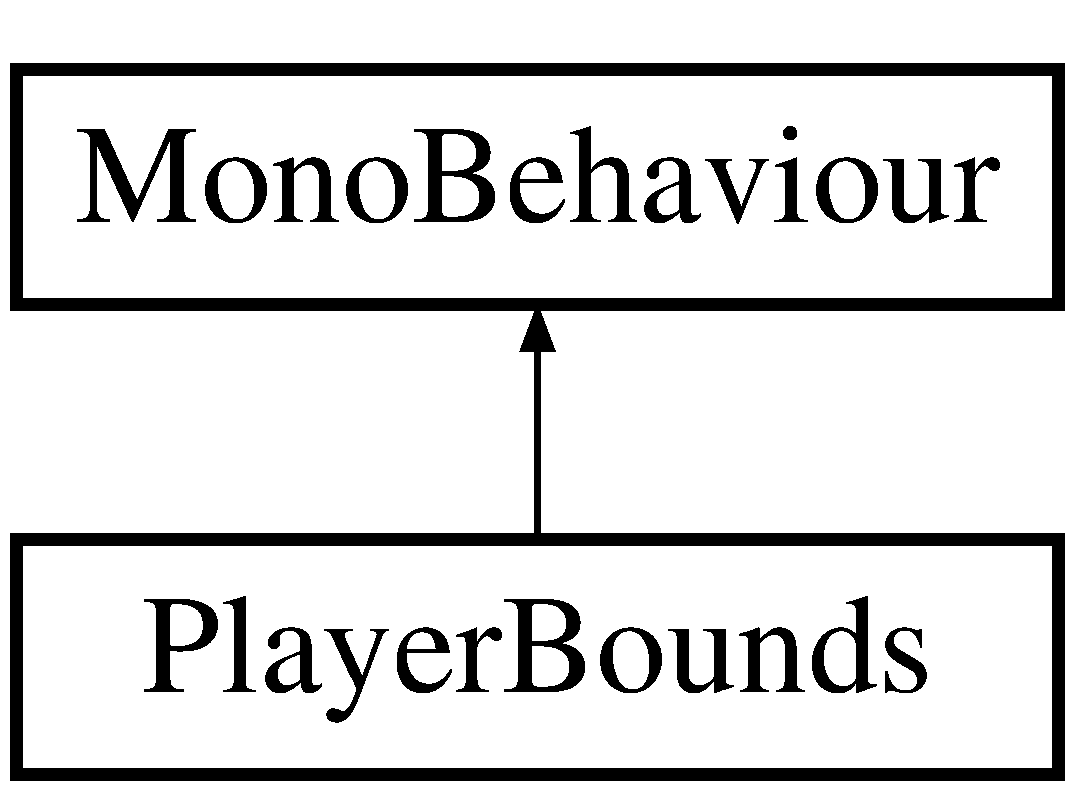
\includegraphics[height=2.000000cm]{class_player_bounds}
\end{center}
\end{figure}
\subsection*{Typy publiczne}
\begin{DoxyCompactItemize}
\item 
enum {\bf Bounds\+Behavior} \{ {\bfseries Nothing}, 
{\bfseries Constrain}, 
{\bfseries Kill}
 \}\begin{DoxyCompactList}\small\item\em Możliwe opcje akcji po przekroczeniu przez gracza dozwolonych granic poziomu, czyli nie robienie niczego, śmierć, lub ograniczenie ruchu. \end{DoxyCompactList}
\end{DoxyCompactItemize}
\subsection*{Metody publiczne}
\begin{DoxyCompactItemize}
\item 
void {\bf Start} ()
\begin{DoxyCompactList}\small\item\em Inicjalizacja obiektu gracza i box collidera. \end{DoxyCompactList}\item 
void {\bf Update} ()
\begin{DoxyCompactList}\small\item\em Korygowanie położenia gracza po przekroczeniu granic poziomu, uwzględniając granice\+: górną, dolną, po prawej stronie ekranu oraz po lewej stronie ekranu. \end{DoxyCompactList}\end{DoxyCompactItemize}
\subsection*{Atrybuty publiczne}
\begin{DoxyCompactItemize}
\item 
Box\+Collider2\+D {\bfseries Bounds}\label{class_player_bounds_a02b847bc2cb2462b058462f8638c02c5}

\item 
{\bf Bounds\+Behavior} {\bfseries Above}\label{class_player_bounds_ab305ba21109a7a08d6f76556ed2beb29}

\item 
{\bf Bounds\+Behavior} {\bfseries Below}\label{class_player_bounds_ae1a36c22e63c4142e1ff336031a783fc}

\item 
{\bf Bounds\+Behavior} {\bfseries Left}\label{class_player_bounds_aba283a79471d6b0b3193a253a6a39df4}

\item 
{\bf Bounds\+Behavior} {\bfseries Right}\label{class_player_bounds_a66f6fea9ec80550b8929561160bd1144}

\end{DoxyCompactItemize}


\subsection{Opis szczegółowy}
Klasa ograniczająca mozliwy ruch gracza jedynie w zakresie widzialnego istniejącego poziomu. 



\subsection{Dokumentacja składowych wyliczanych}
\index{Player\+Bounds@{Player\+Bounds}!Bounds\+Behavior@{Bounds\+Behavior}}
\index{Bounds\+Behavior@{Bounds\+Behavior}!Player\+Bounds@{Player\+Bounds}}
\subsubsection[{Bounds\+Behavior}]{\setlength{\rightskip}{0pt plus 5cm}enum {\bf Player\+Bounds.\+Bounds\+Behavior}\hspace{0.3cm}{\ttfamily [strong]}}\label{class_player_bounds_a5ce066d86d3a67d29e60c4cc10e198ae}


Możliwe opcje akcji po przekroczeniu przez gracza dozwolonych granic poziomu, czyli nie robienie niczego, śmierć, lub ograniczenie ruchu. 



\subsection{Dokumentacja funkcji składowych}
\index{Player\+Bounds@{Player\+Bounds}!Start@{Start}}
\index{Start@{Start}!Player\+Bounds@{Player\+Bounds}}
\subsubsection[{Start()}]{\setlength{\rightskip}{0pt plus 5cm}void Player\+Bounds.\+Start (
\begin{DoxyParamCaption}
{}
\end{DoxyParamCaption}
)}\label{class_player_bounds_aff199ace2c6b71598662d119ba267d20}


Inicjalizacja obiektu gracza i box collidera. 

\index{Player\+Bounds@{Player\+Bounds}!Update@{Update}}
\index{Update@{Update}!Player\+Bounds@{Player\+Bounds}}
\subsubsection[{Update()}]{\setlength{\rightskip}{0pt plus 5cm}void Player\+Bounds.\+Update (
\begin{DoxyParamCaption}
{}
\end{DoxyParamCaption}
)}\label{class_player_bounds_a297bf377a686191be8b798d4e8be1f39}


Korygowanie położenia gracza po przekroczeniu granic poziomu, uwzględniając granice\+: górną, dolną, po prawej stronie ekranu oraz po lewej stronie ekranu. 



Dokumentacja dla tej klasy została wygenerowana z pliku\+:\begin{DoxyCompactItemize}
\item 
C\+:/\+Users/\+Paul/\+Projects/\+Unity\+Game/\+Projekt/\+Assets/\+Code/Player\+Bounds.\+cs\end{DoxyCompactItemize}

\section{Dokumentacja klasy Point\+Star}
\label{class_point_star}\index{Point\+Star@{Point\+Star}}


Klasa przyznająca punkty za zebranie gwiazdek.  


Diagram dziedziczenia dla Point\+Star\begin{figure}[H]
\begin{center}
\leavevmode
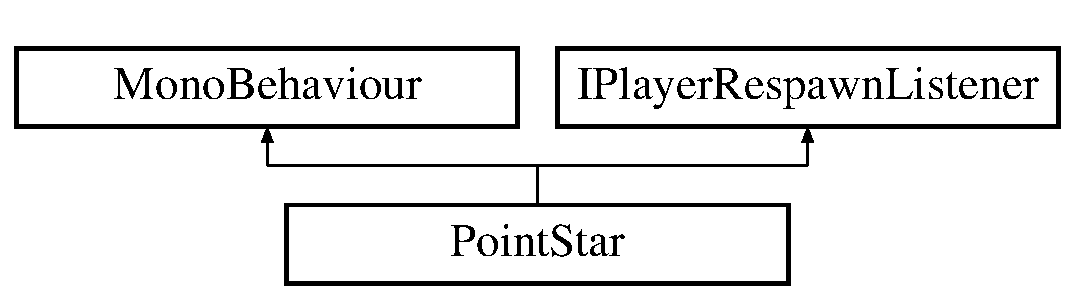
\includegraphics[height=2.000000cm]{class_point_star}
\end{center}
\end{figure}
\subsection*{Metody publiczne}
\begin{DoxyCompactItemize}
\item 
void {\bf On\+Trigger\+Enter2\+D} (Collider2\+D other)
\begin{DoxyCompactList}\small\item\em Po wejściu na gwiazdkę inicjowany jest efekt, a sam obiekt znika. \end{DoxyCompactList}\item 
void {\bf Finish\+Animation\+Event} ()
\begin{DoxyCompactList}\small\item\em Po skończeniu animacji, tekstura jest nieaktywna. \end{DoxyCompactList}\item 
void {\bf On\+Player\+Respawn\+In\+This\+Checkpoint} ({\bf Checkpoint} checkpoint, {\bf Player} player)
\begin{DoxyCompactList}\small\item\em Po respawnie gracza, odtwarzane są gwiazdki zdobyte od czasu osiągnięcia ostatniego checkpointu. \end{DoxyCompactList}\end{DoxyCompactItemize}
\subsection*{Atrybuty publiczne}
\begin{DoxyCompactItemize}
\item 
Game\+Object {\bf Effect}
\begin{DoxyCompactList}\small\item\em Efektem jest chmura żółtych cząsteczek. \end{DoxyCompactList}\item 
int {\bf Points\+To\+Add} = 10
\begin{DoxyCompactList}\small\item\em Liczba punktów dodawana za zebranie gwiazdki. \end{DoxyCompactList}\item 
Audio\+Clip {\bf Hit\+Star\+Sound}
\begin{DoxyCompactList}\small\item\em Dźwięk odtwarzany po zebraniu gwiazdki. \end{DoxyCompactList}\item 
Animator {\bf Animator}
\begin{DoxyCompactList}\small\item\em Obiekt animacji potrzebny do ustawienia efektu przejścia. \end{DoxyCompactList}\item 
Sprite\+Renderer {\bf Renderer}
\begin{DoxyCompactList}\small\item\em Tekstura gwiazdki. \end{DoxyCompactList}\end{DoxyCompactItemize}


\subsection{Opis szczegółowy}
Klasa przyznająca punkty za zebranie gwiazdek. 



\subsection{Dokumentacja funkcji składowych}
\index{Point\+Star@{Point\+Star}!Finish\+Animation\+Event@{Finish\+Animation\+Event}}
\index{Finish\+Animation\+Event@{Finish\+Animation\+Event}!Point\+Star@{Point\+Star}}
\subsubsection[{Finish\+Animation\+Event()}]{\setlength{\rightskip}{0pt plus 5cm}void Point\+Star.\+Finish\+Animation\+Event (
\begin{DoxyParamCaption}
{}
\end{DoxyParamCaption}
)}\label{class_point_star_afbad106da5596521d2876d3fbea805cb}


Po skończeniu animacji, tekstura jest nieaktywna. 

\index{Point\+Star@{Point\+Star}!On\+Player\+Respawn\+In\+This\+Checkpoint@{On\+Player\+Respawn\+In\+This\+Checkpoint}}
\index{On\+Player\+Respawn\+In\+This\+Checkpoint@{On\+Player\+Respawn\+In\+This\+Checkpoint}!Point\+Star@{Point\+Star}}
\subsubsection[{On\+Player\+Respawn\+In\+This\+Checkpoint(\+Checkpoint checkpoint, Player player)}]{\setlength{\rightskip}{0pt plus 5cm}void Point\+Star.\+On\+Player\+Respawn\+In\+This\+Checkpoint (
\begin{DoxyParamCaption}
\item[{{\bf Checkpoint}}]{checkpoint, }
\item[{{\bf Player}}]{player}
\end{DoxyParamCaption}
)}\label{class_point_star_aead5a0a169930cb62f7868873594ba61}


Po respawnie gracza, odtwarzane są gwiazdki zdobyte od czasu osiągnięcia ostatniego checkpointu. 


\begin{DoxyParams}{Parametry}
{\em checkpoint} & \\
\hline
{\em player} & \\
\hline
\end{DoxyParams}


Implementuje {\bf I\+Player\+Respawn\+Listener} \doxyref{}{str.}{interface_i_player_respawn_listener}.

\index{Point\+Star@{Point\+Star}!On\+Trigger\+Enter2\+D@{On\+Trigger\+Enter2\+D}}
\index{On\+Trigger\+Enter2\+D@{On\+Trigger\+Enter2\+D}!Point\+Star@{Point\+Star}}
\subsubsection[{On\+Trigger\+Enter2\+D(\+Collider2\+D other)}]{\setlength{\rightskip}{0pt plus 5cm}void Point\+Star.\+On\+Trigger\+Enter2\+D (
\begin{DoxyParamCaption}
\item[{Collider2\+D}]{other}
\end{DoxyParamCaption}
)}\label{class_point_star_ad146c5292de09a55ba4a7f8b5f3dd8a8}


Po wejściu na gwiazdkę inicjowany jest efekt, a sam obiekt znika. 


\begin{DoxyParams}{Parametry}
{\em other} & \\
\hline
\end{DoxyParams}
Wyjście, jeśli gwiazdka została już zebrana.

Odtworzenie efektu dźwiękowego.

Dodanie punktów.

Inicjowanie efektu graficznego.

Wyświetlenie komunikatu tekstowego.

metoda wyswietli tekst przez 1,5s, bedzie on sie poruszal z predkoscia 50 pixeli na sekunde

Ustawienie gwiazdki jako zebranej. 

\subsection{Dokumentacja atrybutów składowych}
\index{Point\+Star@{Point\+Star}!Animator@{Animator}}
\index{Animator@{Animator}!Point\+Star@{Point\+Star}}
\subsubsection[{Animator}]{\setlength{\rightskip}{0pt plus 5cm}Animator Point\+Star.\+Animator}\label{class_point_star_af6c617a7e1d16f5a5b78fdb7f17ad5f6}


Obiekt animacji potrzebny do ustawienia efektu przejścia. 

\index{Point\+Star@{Point\+Star}!Effect@{Effect}}
\index{Effect@{Effect}!Point\+Star@{Point\+Star}}
\subsubsection[{Effect}]{\setlength{\rightskip}{0pt plus 5cm}Game\+Object Point\+Star.\+Effect}\label{class_point_star_a1e7583d598c88f1f87d61b05efbe643f}


Efektem jest chmura żółtych cząsteczek. 

\index{Point\+Star@{Point\+Star}!Hit\+Star\+Sound@{Hit\+Star\+Sound}}
\index{Hit\+Star\+Sound@{Hit\+Star\+Sound}!Point\+Star@{Point\+Star}}
\subsubsection[{Hit\+Star\+Sound}]{\setlength{\rightskip}{0pt plus 5cm}Audio\+Clip Point\+Star.\+Hit\+Star\+Sound}\label{class_point_star_a2e472961cde18c2d787a8f85e240598f}


Dźwięk odtwarzany po zebraniu gwiazdki. 

\index{Point\+Star@{Point\+Star}!Points\+To\+Add@{Points\+To\+Add}}
\index{Points\+To\+Add@{Points\+To\+Add}!Point\+Star@{Point\+Star}}
\subsubsection[{Points\+To\+Add}]{\setlength{\rightskip}{0pt plus 5cm}int Point\+Star.\+Points\+To\+Add = 10}\label{class_point_star_af7b151a4d96d04019f166538853c3d15}


Liczba punktów dodawana za zebranie gwiazdki. 

\index{Point\+Star@{Point\+Star}!Renderer@{Renderer}}
\index{Renderer@{Renderer}!Point\+Star@{Point\+Star}}
\subsubsection[{Renderer}]{\setlength{\rightskip}{0pt plus 5cm}Sprite\+Renderer Point\+Star.\+Renderer}\label{class_point_star_afa9bbc17daffb816d2d3be058e3e1abd}


Tekstura gwiazdki. 



Dokumentacja dla tej klasy została wygenerowana z pliku\+:\begin{DoxyCompactItemize}
\item 
C\+:/\+Users/\+Paul/\+Projects/\+Unity\+Game/\+Projekt/\+Assets/\+Code/Point\+Star.\+cs\end{DoxyCompactItemize}

\section{Dokumentacja klasy Projectile}
\label{class_projectile}\index{Projectile@{Projectile}}


Podstawowa klasa pocisku.  


Diagram dziedziczenia dla Projectile\begin{figure}[H]
\begin{center}
\leavevmode
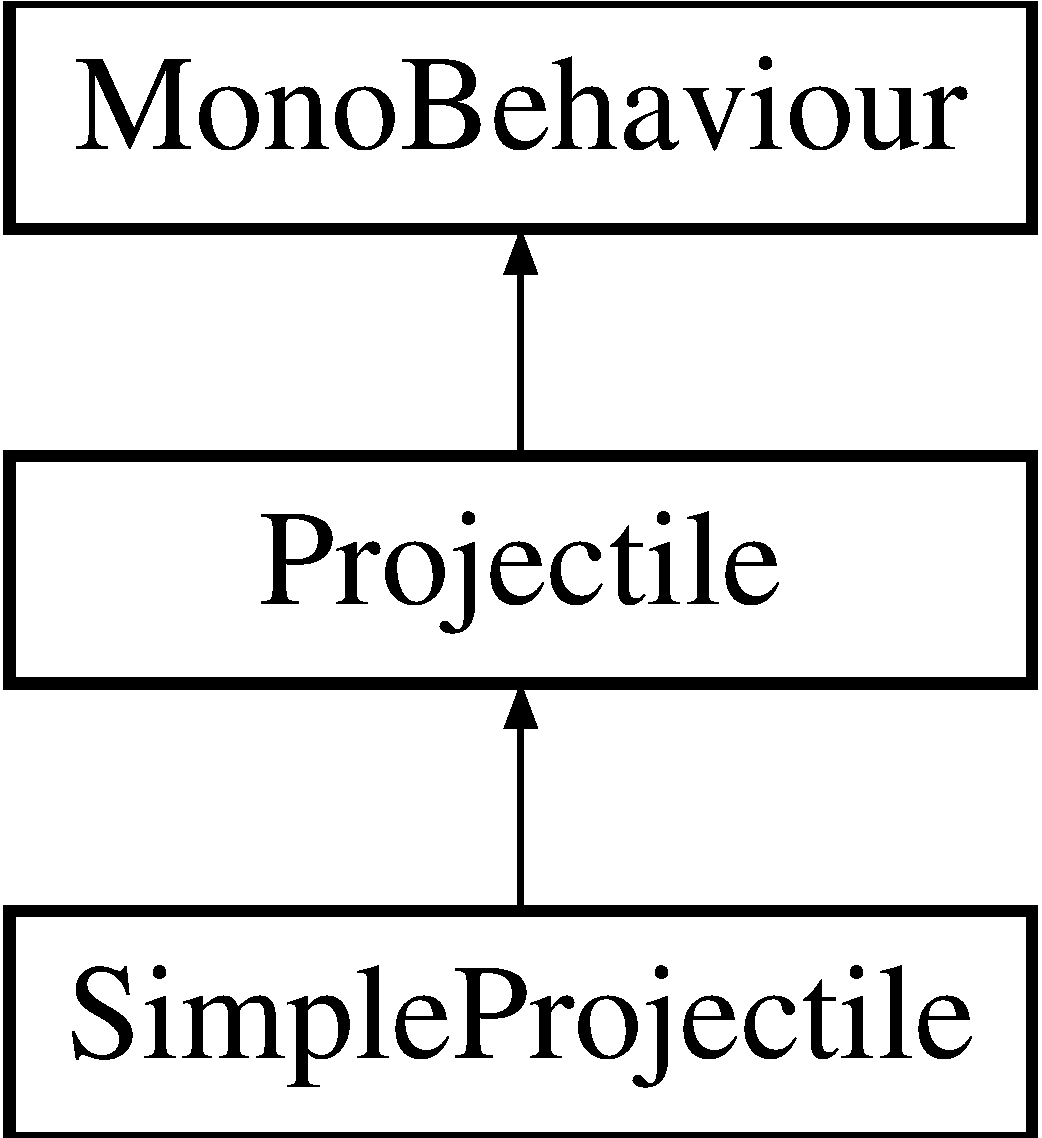
\includegraphics[height=3.000000cm]{class_projectile}
\end{center}
\end{figure}
\subsection*{Metody publiczne}
\begin{DoxyCompactItemize}
\item 
void {\bf Initialize} (Game\+Object owner, Vector2 direction, Vector2 initial\+Velocity)
\begin{DoxyCompactList}\small\item\em Inicjalizacja pocisku, pobierająca kierunek strzału, prędkość obiektu strzelającego, oraz obiekt strzelający jako parametry. \end{DoxyCompactList}\item 
virtual void {\bf On\+Initialized} ()
\begin{DoxyCompactList}\small\item\em Pusta metoda, którą mogą zaimplementować klasy potomne. \end{DoxyCompactList}\item 
virtual void {\bf On\+Trigger\+Enter2\+D} (Collider2\+D other)
\begin{DoxyCompactList}\small\item\em Metoda wywoływana po zderzeniu pocisku z innym obiektem. \end{DoxyCompactList}\end{DoxyCompactItemize}
\subsection*{Atrybuty publiczne}
\begin{DoxyCompactItemize}
\item 
float {\bf Speed}
\begin{DoxyCompactList}\small\item\em Prędkość pocisku. \end{DoxyCompactList}\item 
Layer\+Mask {\bf Collision\+Mask}
\begin{DoxyCompactList}\small\item\em Warstwa kolizji pocisku z otoczeniem. \end{DoxyCompactList}\end{DoxyCompactItemize}
\subsection*{Metody chronione}
\begin{DoxyCompactItemize}
\item 
virtual void {\bf On\+Not\+Collide\+With} (Collider2\+D other)
\begin{DoxyCompactList}\small\item\em Pusta metoda, którą mogą zaimplementować klasy potomne. \end{DoxyCompactList}\item 
virtual void {\bf On\+Collide\+Owner} ()
\begin{DoxyCompactList}\small\item\em Pusta metoda, którą mogą zaimplementować klasy potomne. \end{DoxyCompactList}\item 
virtual void {\bf On\+Collide\+Take\+Damage} (Collider2\+D other, {\bf I\+Take\+Damage} take\+Damage)
\begin{DoxyCompactList}\small\item\em Pusta metoda, którą mogą zaimplementować klasy potomne. \end{DoxyCompactList}\item 
virtual void {\bf On\+Collide\+Other} (Collider2\+D other)
\begin{DoxyCompactList}\small\item\em Pusta metoda, którą mogą zaimplementować klasy potomne. \end{DoxyCompactList}\end{DoxyCompactItemize}
\subsection*{Właściwości}
\begin{DoxyCompactItemize}
\item 
Game\+Object {\bf Owner}\hspace{0.3cm}{\ttfamily  [get]}
\begin{DoxyCompactList}\small\item\em Obiekt, który wystrzeli pocisk. \end{DoxyCompactList}\item 
Vector2 {\bf Direction}\hspace{0.3cm}{\ttfamily  [get]}
\begin{DoxyCompactList}\small\item\em Kierunek strzału. \end{DoxyCompactList}\item 
Vector2 {\bf Initial\+Velocity}\hspace{0.3cm}{\ttfamily  [get]}
\begin{DoxyCompactList}\small\item\em Prędkość obiektu-\/właściciela pocisku, która później jest dodawana do prędkości pocisku podczas wystrzału. \end{DoxyCompactList}\end{DoxyCompactItemize}


\subsection{Opis szczegółowy}
Podstawowa klasa pocisku. 



\subsection{Dokumentacja funkcji składowych}
\index{Projectile@{Projectile}!Initialize@{Initialize}}
\index{Initialize@{Initialize}!Projectile@{Projectile}}
\subsubsection[{Initialize(\+Game\+Object owner, Vector2 direction, Vector2 initial\+Velocity)}]{\setlength{\rightskip}{0pt plus 5cm}void Projectile.\+Initialize (
\begin{DoxyParamCaption}
\item[{Game\+Object}]{owner, }
\item[{Vector2}]{direction, }
\item[{Vector2}]{initial\+Velocity}
\end{DoxyParamCaption}
)}\label{class_projectile_a3e3cdf6fcfd15893d63623affc270ded}


Inicjalizacja pocisku, pobierająca kierunek strzału, prędkość obiektu strzelającego, oraz obiekt strzelający jako parametry. 


\begin{DoxyParams}{Parametry}
{\em owner} & \\
\hline
{\em direction} & \\
\hline
{\em initial\+Velocity} & \\
\hline
\end{DoxyParams}
Ustawienie kierunku pocisku.

Ustawienie obiektu oddającego strzał.

Ustawienie kierunku strzału.

Ustawienie początkowej prędkości strzału. \index{Projectile@{Projectile}!On\+Collide\+Other@{On\+Collide\+Other}}
\index{On\+Collide\+Other@{On\+Collide\+Other}!Projectile@{Projectile}}
\subsubsection[{On\+Collide\+Other(\+Collider2\+D other)}]{\setlength{\rightskip}{0pt plus 5cm}virtual void Projectile.\+On\+Collide\+Other (
\begin{DoxyParamCaption}
\item[{Collider2\+D}]{other}
\end{DoxyParamCaption}
)\hspace{0.3cm}{\ttfamily [protected]}, {\ttfamily [virtual]}}\label{class_projectile_ad7deb35a74b4a3ee934d554b419d63af}


Pusta metoda, którą mogą zaimplementować klasy potomne. 


\begin{DoxyParams}{Parametry}
{\em other} & \\
\hline
\end{DoxyParams}


Reimplementowana w {\bf Simple\+Projectile} \doxyref{}{str.}{class_simple_projectile_a51baf8e9ef7543293b810f12a6882db0}.

\index{Projectile@{Projectile}!On\+Collide\+Owner@{On\+Collide\+Owner}}
\index{On\+Collide\+Owner@{On\+Collide\+Owner}!Projectile@{Projectile}}
\subsubsection[{On\+Collide\+Owner()}]{\setlength{\rightskip}{0pt plus 5cm}virtual void Projectile.\+On\+Collide\+Owner (
\begin{DoxyParamCaption}
{}
\end{DoxyParamCaption}
)\hspace{0.3cm}{\ttfamily [protected]}, {\ttfamily [virtual]}}\label{class_projectile_a0f7dd0259be773db60a3cd6fca06e8bd}


Pusta metoda, którą mogą zaimplementować klasy potomne. 

\index{Projectile@{Projectile}!On\+Collide\+Take\+Damage@{On\+Collide\+Take\+Damage}}
\index{On\+Collide\+Take\+Damage@{On\+Collide\+Take\+Damage}!Projectile@{Projectile}}
\subsubsection[{On\+Collide\+Take\+Damage(\+Collider2\+D other, I\+Take\+Damage take\+Damage)}]{\setlength{\rightskip}{0pt plus 5cm}virtual void Projectile.\+On\+Collide\+Take\+Damage (
\begin{DoxyParamCaption}
\item[{Collider2\+D}]{other, }
\item[{{\bf I\+Take\+Damage}}]{take\+Damage}
\end{DoxyParamCaption}
)\hspace{0.3cm}{\ttfamily [protected]}, {\ttfamily [virtual]}}\label{class_projectile_adafb479f251df04ac62f3806d542780b}


Pusta metoda, którą mogą zaimplementować klasy potomne. 


\begin{DoxyParams}{Parametry}
{\em other} & \\
\hline
{\em take\+Damage} & \\
\hline
\end{DoxyParams}


Reimplementowana w {\bf Simple\+Projectile} \doxyref{}{str.}{class_simple_projectile_ab720e692e4fbc643d8ffc86f40636a67}.

\index{Projectile@{Projectile}!On\+Initialized@{On\+Initialized}}
\index{On\+Initialized@{On\+Initialized}!Projectile@{Projectile}}
\subsubsection[{On\+Initialized()}]{\setlength{\rightskip}{0pt plus 5cm}virtual void Projectile.\+On\+Initialized (
\begin{DoxyParamCaption}
{}
\end{DoxyParamCaption}
)\hspace{0.3cm}{\ttfamily [virtual]}}\label{class_projectile_a624c604c99612d5f770e7933398926e9}


Pusta metoda, którą mogą zaimplementować klasy potomne. 

\index{Projectile@{Projectile}!On\+Not\+Collide\+With@{On\+Not\+Collide\+With}}
\index{On\+Not\+Collide\+With@{On\+Not\+Collide\+With}!Projectile@{Projectile}}
\subsubsection[{On\+Not\+Collide\+With(\+Collider2\+D other)}]{\setlength{\rightskip}{0pt plus 5cm}virtual void Projectile.\+On\+Not\+Collide\+With (
\begin{DoxyParamCaption}
\item[{Collider2\+D}]{other}
\end{DoxyParamCaption}
)\hspace{0.3cm}{\ttfamily [protected]}, {\ttfamily [virtual]}}\label{class_projectile_aed16cdf72286c332c5cee2933706ca97}


Pusta metoda, którą mogą zaimplementować klasy potomne. 


\begin{DoxyParams}{Parametry}
{\em other} & \\
\hline
\end{DoxyParams}
\index{Projectile@{Projectile}!On\+Trigger\+Enter2\+D@{On\+Trigger\+Enter2\+D}}
\index{On\+Trigger\+Enter2\+D@{On\+Trigger\+Enter2\+D}!Projectile@{Projectile}}
\subsubsection[{On\+Trigger\+Enter2\+D(\+Collider2\+D other)}]{\setlength{\rightskip}{0pt plus 5cm}virtual void Projectile.\+On\+Trigger\+Enter2\+D (
\begin{DoxyParamCaption}
\item[{Collider2\+D}]{other}
\end{DoxyParamCaption}
)\hspace{0.3cm}{\ttfamily [virtual]}}\label{class_projectile_a107df718306594b9e793879cafcc1072}


Metoda wywoływana po zderzeniu pocisku z innym obiektem. 


\begin{DoxyParams}{Parametry}
{\em other} & \\
\hline
\end{DoxyParams}
Pocisk zderzył się z czymś, co nie odpowiada masce kolizji.

Pocisk zderzył się z obiektem, który wystrzelił pocisk.

Pocisk zderzył się z obiektem, który może przyjmować obrażenia.

Żadne z powyższych. 

\subsection{Dokumentacja atrybutów składowych}
\index{Projectile@{Projectile}!Collision\+Mask@{Collision\+Mask}}
\index{Collision\+Mask@{Collision\+Mask}!Projectile@{Projectile}}
\subsubsection[{Collision\+Mask}]{\setlength{\rightskip}{0pt plus 5cm}Layer\+Mask Projectile.\+Collision\+Mask}\label{class_projectile_a45d75a6361f9a64b50291ab84622bcac}


Warstwa kolizji pocisku z otoczeniem. 

\index{Projectile@{Projectile}!Speed@{Speed}}
\index{Speed@{Speed}!Projectile@{Projectile}}
\subsubsection[{Speed}]{\setlength{\rightskip}{0pt plus 5cm}float Projectile.\+Speed}\label{class_projectile_a635b74f687fe3e37f8602bb18d13f90f}


Prędkość pocisku. 



\subsection{Dokumentacja właściwości}
\index{Projectile@{Projectile}!Direction@{Direction}}
\index{Direction@{Direction}!Projectile@{Projectile}}
\subsubsection[{Direction}]{\setlength{\rightskip}{0pt plus 5cm}Vector2 Projectile.\+Direction\hspace{0.3cm}{\ttfamily [get]}}\label{class_projectile_a117a5b2f9a9e05cd541a949d47f8d83c}


Kierunek strzału. 

\index{Projectile@{Projectile}!Initial\+Velocity@{Initial\+Velocity}}
\index{Initial\+Velocity@{Initial\+Velocity}!Projectile@{Projectile}}
\subsubsection[{Initial\+Velocity}]{\setlength{\rightskip}{0pt plus 5cm}Vector2 Projectile.\+Initial\+Velocity\hspace{0.3cm}{\ttfamily [get]}}\label{class_projectile_a7a9f5f3770332c4cbd42afc1e33cddff}


Prędkość obiektu-\/właściciela pocisku, która później jest dodawana do prędkości pocisku podczas wystrzału. 

\index{Projectile@{Projectile}!Owner@{Owner}}
\index{Owner@{Owner}!Projectile@{Projectile}}
\subsubsection[{Owner}]{\setlength{\rightskip}{0pt plus 5cm}Game\+Object Projectile.\+Owner\hspace{0.3cm}{\ttfamily [get]}}\label{class_projectile_a5599c73fed5fdef2a40e2a5abd6e013a}


Obiekt, który wystrzeli pocisk. 



Dokumentacja dla tej klasy została wygenerowana z pliku\+:\begin{DoxyCompactItemize}
\item 
C\+:/\+Users/\+Paul/\+Projects/\+Unity\+Game/\+Projekt/\+Assets/\+Code/Projectile.\+cs\end{DoxyCompactItemize}

\section{Dokumentacja klasy Simple\+Enemy\+Ai}
\label{class_simple_enemy_ai}\index{Simple\+Enemy\+Ai@{Simple\+Enemy\+Ai}}


Klasa odpowiadająca za podstawowe działania przeciwnika w świecie gry.  


Diagram dziedziczenia dla Simple\+Enemy\+Ai\begin{figure}[H]
\begin{center}
\leavevmode
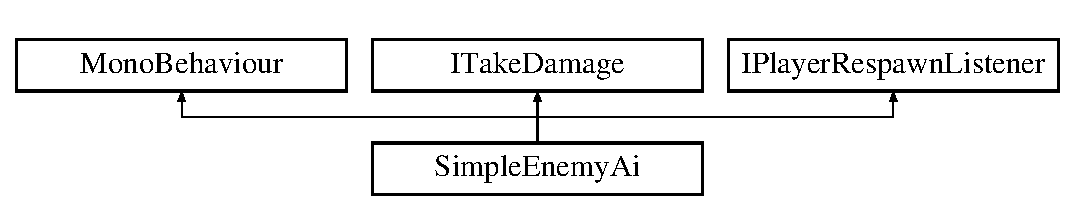
\includegraphics[height=2.000000cm]{class_simple_enemy_ai}
\end{center}
\end{figure}
\subsection*{Metody publiczne}
\begin{DoxyCompactItemize}
\item 
void {\bf Start} ()
\begin{DoxyCompactList}\small\item\em Ustawienie parametrów początkowych\+: kontrolera, kierunku i pozycji początkowej. \end{DoxyCompactList}\item 
void {\bf Update} ()
\begin{DoxyCompactList}\small\item\em Aktualizacja położenia przeciwnika oraz obsługa strzelania pociskami. \end{DoxyCompactList}\item 
void {\bf Take\+Damage} (int damage, Game\+Object instigator)
\begin{DoxyCompactList}\small\item\em Metoda wywoływana po otrzymaniu obrażeń od gracza. \end{DoxyCompactList}\item 
void {\bf On\+Player\+Respawn\+In\+This\+Checkpoint} ({\bf Checkpoint} checkpoint, {\bf Player} player)
\begin{DoxyCompactList}\small\item\em Zrespawnowanie przeciwnika w danym checkpoincie razem z graczem. \end{DoxyCompactList}\end{DoxyCompactItemize}
\subsection*{Atrybuty publiczne}
\begin{DoxyCompactItemize}
\item 
float {\bf Speed}
\begin{DoxyCompactList}\small\item\em Prędkość przeciwnika. \end{DoxyCompactList}\item 
float {\bf Fire\+Rate} = 1
\begin{DoxyCompactList}\small\item\em Częstotliwość oddawania strzałów przez przeciwnika. \end{DoxyCompactList}\item 
{\bf Projectile} {\bf Projectile}
\begin{DoxyCompactList}\small\item\em Pocisk. \end{DoxyCompactList}\item 
Game\+Object {\bf Destroyed\+Effect}
\begin{DoxyCompactList}\small\item\em Efekt zniszczenia przeciwnika. \end{DoxyCompactList}\item 
int {\bf Points\+To\+Give\+Player}
\begin{DoxyCompactList}\small\item\em Punkty przyznawane graczowi za zestrzelenie przeciwnika. \end{DoxyCompactList}\item 
Audio\+Clip {\bf Shoot\+Sound}
\begin{DoxyCompactList}\small\item\em Dwięk strzału przeciwnika. \end{DoxyCompactList}\end{DoxyCompactItemize}


\subsection{Opis szczegółowy}
Klasa odpowiadająca za podstawowe działania przeciwnika w świecie gry. 



\subsection{Dokumentacja funkcji składowych}
\index{Simple\+Enemy\+Ai@{Simple\+Enemy\+Ai}!On\+Player\+Respawn\+In\+This\+Checkpoint@{On\+Player\+Respawn\+In\+This\+Checkpoint}}
\index{On\+Player\+Respawn\+In\+This\+Checkpoint@{On\+Player\+Respawn\+In\+This\+Checkpoint}!Simple\+Enemy\+Ai@{Simple\+Enemy\+Ai}}
\subsubsection[{On\+Player\+Respawn\+In\+This\+Checkpoint(\+Checkpoint checkpoint, Player player)}]{\setlength{\rightskip}{0pt plus 5cm}void Simple\+Enemy\+Ai.\+On\+Player\+Respawn\+In\+This\+Checkpoint (
\begin{DoxyParamCaption}
\item[{{\bf Checkpoint}}]{checkpoint, }
\item[{{\bf Player}}]{player}
\end{DoxyParamCaption}
)}\label{class_simple_enemy_ai_ad4045de41577b6232f046d710f2971a4}


Zrespawnowanie przeciwnika w danym checkpoincie razem z graczem. 


\begin{DoxyParams}{Parametry}
{\em checkpoint} & \\
\hline
{\em player} & \\
\hline
\end{DoxyParams}
Ustawienie jego kierunku.

Ustawienie jego skali w świecie gry jako domyœlnej.

Ustawienie pozycji początkowej.

Aktywowanie obiektu przeciwnika w świecie gry. 

Implementuje {\bf I\+Player\+Respawn\+Listener} \doxyref{}{str.}{interface_i_player_respawn_listener}.

\index{Simple\+Enemy\+Ai@{Simple\+Enemy\+Ai}!Start@{Start}}
\index{Start@{Start}!Simple\+Enemy\+Ai@{Simple\+Enemy\+Ai}}
\subsubsection[{Start()}]{\setlength{\rightskip}{0pt plus 5cm}void Simple\+Enemy\+Ai.\+Start (
\begin{DoxyParamCaption}
{}
\end{DoxyParamCaption}
)}\label{class_simple_enemy_ai_a64a4274eed9b9b586c7ec70d0066a727}


Ustawienie parametrów początkowych\+: kontrolera, kierunku i pozycji początkowej. 

Domyślnie porusza się w lewo. \index{Simple\+Enemy\+Ai@{Simple\+Enemy\+Ai}!Take\+Damage@{Take\+Damage}}
\index{Take\+Damage@{Take\+Damage}!Simple\+Enemy\+Ai@{Simple\+Enemy\+Ai}}
\subsubsection[{Take\+Damage(int damage, Game\+Object instigator)}]{\setlength{\rightskip}{0pt plus 5cm}void Simple\+Enemy\+Ai.\+Take\+Damage (
\begin{DoxyParamCaption}
\item[{int}]{damage, }
\item[{Game\+Object}]{instigator}
\end{DoxyParamCaption}
)}\label{class_simple_enemy_ai_a06d025942faa857d353febf6f217bcdc}


Metoda wywoływana po otrzymaniu obrażeń od gracza. 


\begin{DoxyParams}{Parametry}
{\em damage} & \\
\hline
{\em instigator} & \\
\hline
\end{DoxyParams}
Przyznanie punktów graczowi za zestrzelenie wroga.

Uruchomeinie efektu zestrzelenia przeciwnika.

Ustawienie obiektu przeciwnika jako niekatywnego. 

Implementuje {\bf I\+Take\+Damage} \doxyref{}{str.}{interface_i_take_damage}.

\index{Simple\+Enemy\+Ai@{Simple\+Enemy\+Ai}!Update@{Update}}
\index{Update@{Update}!Simple\+Enemy\+Ai@{Simple\+Enemy\+Ai}}
\subsubsection[{Update()}]{\setlength{\rightskip}{0pt plus 5cm}void Simple\+Enemy\+Ai.\+Update (
\begin{DoxyParamCaption}
{}
\end{DoxyParamCaption}
)}\label{class_simple_enemy_ai_a8e8cd468827d9edd2b337002d55ade58}


Aktualizacja położenia przeciwnika oraz obsługa strzelania pociskami. 

Wykonanie ruchu przez przeciwnika.

Po napotkaniu przeszkody, przeciwnik porusza się w odwrotnym kierunku.

Sprawdzenie czy upłynął czas potrzebny do wystrzelenia nowrgo pocisku.

Sprawdzenie czy gracz zostaje trafiony przez pocisk (jest w zasięgu strzału przeciwnika).

Stworzenie zmiennej pocisku.

Inicjalizacja pocisku z ustawioną prędkością i kierunkiem.

Ustawienie częstotliowości oddawania strzałów.

Uruchomienie dźwięku wystrzału pocisku przez przeciwnika. 

\subsection{Dokumentacja atrybutów składowych}
\index{Simple\+Enemy\+Ai@{Simple\+Enemy\+Ai}!Destroyed\+Effect@{Destroyed\+Effect}}
\index{Destroyed\+Effect@{Destroyed\+Effect}!Simple\+Enemy\+Ai@{Simple\+Enemy\+Ai}}
\subsubsection[{Destroyed\+Effect}]{\setlength{\rightskip}{0pt plus 5cm}Game\+Object Simple\+Enemy\+Ai.\+Destroyed\+Effect}\label{class_simple_enemy_ai_ab3acba0e0566f03ff2512182f453f423}


Efekt zniszczenia przeciwnika. 

\index{Simple\+Enemy\+Ai@{Simple\+Enemy\+Ai}!Fire\+Rate@{Fire\+Rate}}
\index{Fire\+Rate@{Fire\+Rate}!Simple\+Enemy\+Ai@{Simple\+Enemy\+Ai}}
\subsubsection[{Fire\+Rate}]{\setlength{\rightskip}{0pt plus 5cm}float Simple\+Enemy\+Ai.\+Fire\+Rate = 1}\label{class_simple_enemy_ai_a1798faa2837dca4a9ab935bebac1a295}


Częstotliwość oddawania strzałów przez przeciwnika. 

\index{Simple\+Enemy\+Ai@{Simple\+Enemy\+Ai}!Points\+To\+Give\+Player@{Points\+To\+Give\+Player}}
\index{Points\+To\+Give\+Player@{Points\+To\+Give\+Player}!Simple\+Enemy\+Ai@{Simple\+Enemy\+Ai}}
\subsubsection[{Points\+To\+Give\+Player}]{\setlength{\rightskip}{0pt plus 5cm}int Simple\+Enemy\+Ai.\+Points\+To\+Give\+Player}\label{class_simple_enemy_ai_ad82e14f2330c7c180a10b66bd83de177}


Punkty przyznawane graczowi za zestrzelenie przeciwnika. 

\index{Simple\+Enemy\+Ai@{Simple\+Enemy\+Ai}!Projectile@{Projectile}}
\index{Projectile@{Projectile}!Simple\+Enemy\+Ai@{Simple\+Enemy\+Ai}}
\subsubsection[{Projectile}]{\setlength{\rightskip}{0pt plus 5cm}{\bf Projectile} Simple\+Enemy\+Ai.\+Projectile}\label{class_simple_enemy_ai_a26027ac987933b4aaadeb94c51bccbb3}


Pocisk. 

\index{Simple\+Enemy\+Ai@{Simple\+Enemy\+Ai}!Shoot\+Sound@{Shoot\+Sound}}
\index{Shoot\+Sound@{Shoot\+Sound}!Simple\+Enemy\+Ai@{Simple\+Enemy\+Ai}}
\subsubsection[{Shoot\+Sound}]{\setlength{\rightskip}{0pt plus 5cm}Audio\+Clip Simple\+Enemy\+Ai.\+Shoot\+Sound}\label{class_simple_enemy_ai_a924901f31131a3b8fb3fff3e39ccb927}


Dwięk strzału przeciwnika. 

\index{Simple\+Enemy\+Ai@{Simple\+Enemy\+Ai}!Speed@{Speed}}
\index{Speed@{Speed}!Simple\+Enemy\+Ai@{Simple\+Enemy\+Ai}}
\subsubsection[{Speed}]{\setlength{\rightskip}{0pt plus 5cm}float Simple\+Enemy\+Ai.\+Speed}\label{class_simple_enemy_ai_a78b91ea3da1dc65b7f93eadc8ef1d8e6}


Prędkość przeciwnika. 



Dokumentacja dla tej klasy została wygenerowana z pliku\+:\begin{DoxyCompactItemize}
\item 
C\+:/\+Users/\+Paul/\+Projects/\+Unity\+Game/\+Projekt/\+Assets/\+Code/Simple\+Enemy\+Ai.\+cs\end{DoxyCompactItemize}

\section{Dokumentacja klasy Simple\+Projectile}
\label{class_simple_projectile}\index{Simple\+Projectile@{Simple\+Projectile}}


Klasa potomna dziedzicząca z \doxyref{Projectile}{str.}{class_projectile}.  


Diagram dziedziczenia dla Simple\+Projectile\begin{figure}[H]
\begin{center}
\leavevmode
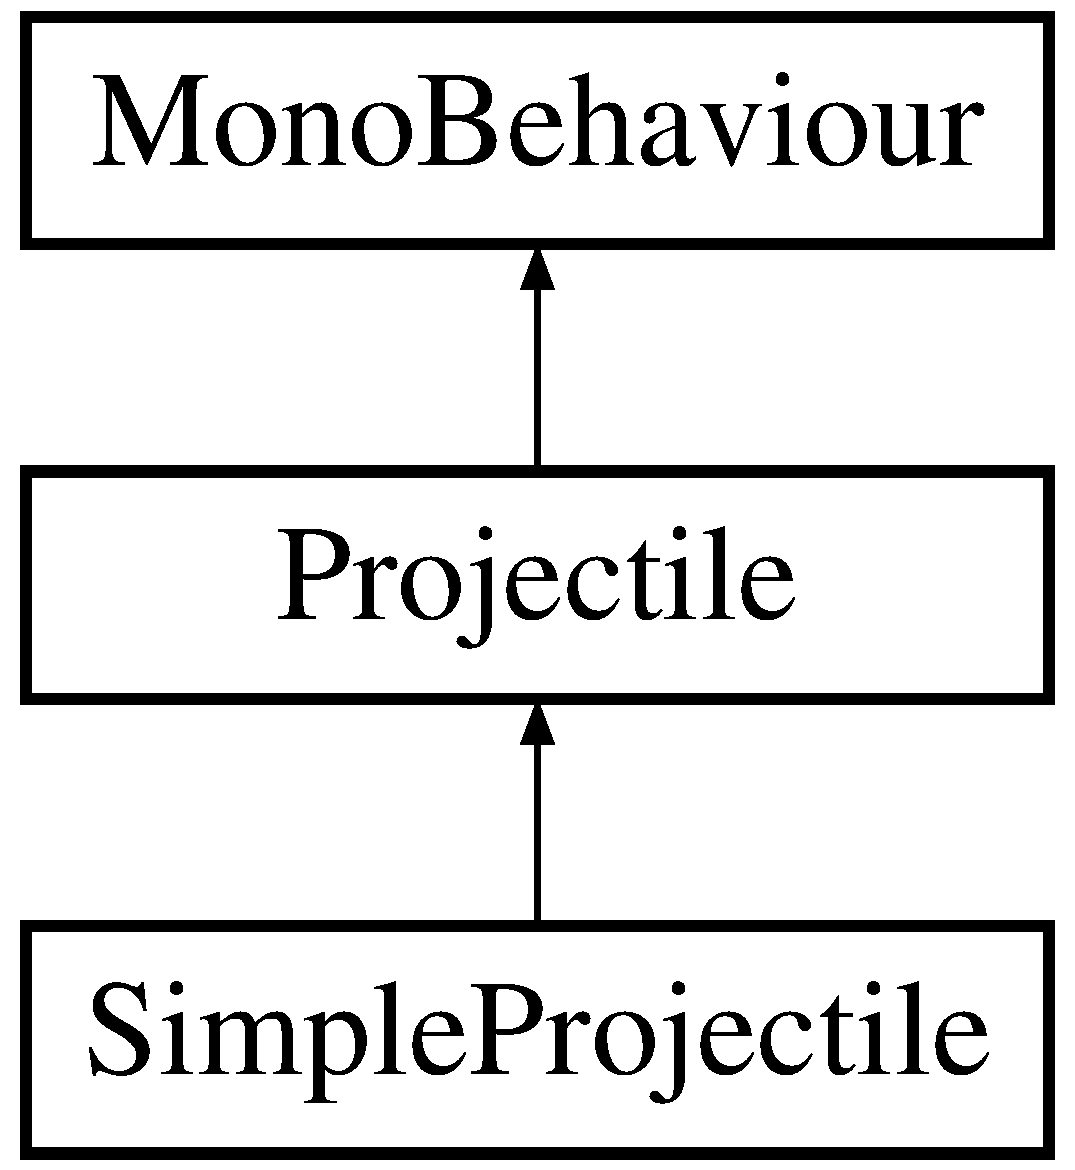
\includegraphics[height=3.000000cm]{class_simple_projectile}
\end{center}
\end{figure}
\subsection*{Metody publiczne}
\begin{DoxyCompactItemize}
\item 
void {\bf Update} ()
\begin{DoxyCompactList}\small\item\em Metoda aktualizująca pozycję pocisku w Unity, oraz odpowiadająca za jego zniszczenie po upływie czasu życia pocisku. \end{DoxyCompactList}\item 
void {\bf Take\+Damage} (int damage, Game\+Object instigator)
\begin{DoxyCompactList}\small\item\em Metoda odpowiadająca za zniszczenie pocisku i przyznanie punktów graczowi, jesli uda mu się zestrzelić pocisk przeciwnika. \end{DoxyCompactList}\end{DoxyCompactItemize}
\subsection*{Atrybuty publiczne}
\begin{DoxyCompactItemize}
\item 
int {\bf Damage}
\begin{DoxyCompactList}\small\item\em Obrażenia zadane przez pocisk. \end{DoxyCompactList}\item 
Game\+Object {\bf Destroyed\+Effect}
\begin{DoxyCompactList}\small\item\em Efekt zniszczenia pocisku. \end{DoxyCompactList}\item 
int {\bf Points\+To\+Give\+To\+Player}
\begin{DoxyCompactList}\small\item\em Punkty przyznawane graczowi, jeśli uda mu się zniszczyć (w locie) pocisk przeciwnika. \end{DoxyCompactList}\item 
float {\bf Time\+To\+Live}
\begin{DoxyCompactList}\small\item\em Czas życia pocisku. \end{DoxyCompactList}\item 
Audio\+Clip {\bf Destroy\+Sound}
\begin{DoxyCompactList}\small\item\em Dźwięk odtwarzany przy zniszczeniu pocisku \end{DoxyCompactList}\end{DoxyCompactItemize}
\subsection*{Metody chronione}
\begin{DoxyCompactItemize}
\item 
override void {\bf On\+Collide\+Other} (Collider2\+D other)
\begin{DoxyCompactList}\small\item\em Podczas kolizji z otoczeniem nastąpi zniszczenie pocisku. \end{DoxyCompactList}\item 
override void {\bf On\+Collide\+Take\+Damage} (Collider2\+D other, {\bf I\+Take\+Damage} take\+Damage)
\begin{DoxyCompactList}\small\item\em Metoda wywoływana po trafieniu przez pocisk obiektu, który może przyjąć obrażenia. \end{DoxyCompactList}\end{DoxyCompactItemize}
\subsection*{Dodatkowe Dziedziczone Składowe}


\subsection{Opis szczegółowy}
Klasa potomna dziedzicząca z \doxyref{Projectile}{str.}{class_projectile}. 



\subsection{Dokumentacja funkcji składowych}
\index{Simple\+Projectile@{Simple\+Projectile}!On\+Collide\+Other@{On\+Collide\+Other}}
\index{On\+Collide\+Other@{On\+Collide\+Other}!Simple\+Projectile@{Simple\+Projectile}}
\subsubsection[{On\+Collide\+Other(\+Collider2\+D other)}]{\setlength{\rightskip}{0pt plus 5cm}override void Simple\+Projectile.\+On\+Collide\+Other (
\begin{DoxyParamCaption}
\item[{Collider2\+D}]{other}
\end{DoxyParamCaption}
)\hspace{0.3cm}{\ttfamily [protected]}, {\ttfamily [virtual]}}\label{class_simple_projectile_a51baf8e9ef7543293b810f12a6882db0}


Podczas kolizji z otoczeniem nastąpi zniszczenie pocisku. 


\begin{DoxyParams}{Parametry}
{\em other} & \\
\hline
\end{DoxyParams}


Reimplementowana z {\bf Projectile} \doxyref{}{str.}{class_projectile_ad7deb35a74b4a3ee934d554b419d63af}.

\index{Simple\+Projectile@{Simple\+Projectile}!On\+Collide\+Take\+Damage@{On\+Collide\+Take\+Damage}}
\index{On\+Collide\+Take\+Damage@{On\+Collide\+Take\+Damage}!Simple\+Projectile@{Simple\+Projectile}}
\subsubsection[{On\+Collide\+Take\+Damage(\+Collider2\+D other, I\+Take\+Damage take\+Damage)}]{\setlength{\rightskip}{0pt plus 5cm}override void Simple\+Projectile.\+On\+Collide\+Take\+Damage (
\begin{DoxyParamCaption}
\item[{Collider2\+D}]{other, }
\item[{{\bf I\+Take\+Damage}}]{take\+Damage}
\end{DoxyParamCaption}
)\hspace{0.3cm}{\ttfamily [protected]}, {\ttfamily [virtual]}}\label{class_simple_projectile_ab720e692e4fbc643d8ffc86f40636a67}


Metoda wywoływana po trafieniu przez pocisk obiektu, który może przyjąć obrażenia. 


\begin{DoxyParams}{Parametry}
{\em other} & \\
\hline
{\em take\+Damage} & \\
\hline
\end{DoxyParams}


Reimplementowana z {\bf Projectile} \doxyref{}{str.}{class_projectile_adafb479f251df04ac62f3806d542780b}.

\index{Simple\+Projectile@{Simple\+Projectile}!Take\+Damage@{Take\+Damage}}
\index{Take\+Damage@{Take\+Damage}!Simple\+Projectile@{Simple\+Projectile}}
\subsubsection[{Take\+Damage(int damage, Game\+Object instigator)}]{\setlength{\rightskip}{0pt plus 5cm}void Simple\+Projectile.\+Take\+Damage (
\begin{DoxyParamCaption}
\item[{int}]{damage, }
\item[{Game\+Object}]{instigator}
\end{DoxyParamCaption}
)}\label{class_simple_projectile_a5140d89a2b093bb3659777ac18b1d5c2}


Metoda odpowiadająca za zniszczenie pocisku i przyznanie punktów graczowi, jesli uda mu się zestrzelić pocisk przeciwnika. 


\begin{DoxyParams}{Parametry}
{\em damage} & \\
\hline
{\em instigator} & \\
\hline
\end{DoxyParams}
\index{Simple\+Projectile@{Simple\+Projectile}!Update@{Update}}
\index{Update@{Update}!Simple\+Projectile@{Simple\+Projectile}}
\subsubsection[{Update()}]{\setlength{\rightskip}{0pt plus 5cm}void Simple\+Projectile.\+Update (
\begin{DoxyParamCaption}
{}
\end{DoxyParamCaption}
)}\label{class_simple_projectile_a528563fe128025104799641725d3bf4e}


Metoda aktualizująca pozycję pocisku w Unity, oraz odpowiadająca za jego zniszczenie po upływie czasu życia pocisku. 



\subsection{Dokumentacja atrybutów składowych}
\index{Simple\+Projectile@{Simple\+Projectile}!Damage@{Damage}}
\index{Damage@{Damage}!Simple\+Projectile@{Simple\+Projectile}}
\subsubsection[{Damage}]{\setlength{\rightskip}{0pt plus 5cm}int Simple\+Projectile.\+Damage}\label{class_simple_projectile_a038f4726ab80eed50b1d511e10b0f553}


Obrażenia zadane przez pocisk. 

\index{Simple\+Projectile@{Simple\+Projectile}!Destroyed\+Effect@{Destroyed\+Effect}}
\index{Destroyed\+Effect@{Destroyed\+Effect}!Simple\+Projectile@{Simple\+Projectile}}
\subsubsection[{Destroyed\+Effect}]{\setlength{\rightskip}{0pt plus 5cm}Game\+Object Simple\+Projectile.\+Destroyed\+Effect}\label{class_simple_projectile_af9be68e8d9ffdf298339c5ec0964630e}


Efekt zniszczenia pocisku. 

\index{Simple\+Projectile@{Simple\+Projectile}!Destroy\+Sound@{Destroy\+Sound}}
\index{Destroy\+Sound@{Destroy\+Sound}!Simple\+Projectile@{Simple\+Projectile}}
\subsubsection[{Destroy\+Sound}]{\setlength{\rightskip}{0pt plus 5cm}Audio\+Clip Simple\+Projectile.\+Destroy\+Sound}\label{class_simple_projectile_a2c36fea359143d0884e8530e63828246}


Dźwięk odtwarzany przy zniszczeniu pocisku 

\index{Simple\+Projectile@{Simple\+Projectile}!Points\+To\+Give\+To\+Player@{Points\+To\+Give\+To\+Player}}
\index{Points\+To\+Give\+To\+Player@{Points\+To\+Give\+To\+Player}!Simple\+Projectile@{Simple\+Projectile}}
\subsubsection[{Points\+To\+Give\+To\+Player}]{\setlength{\rightskip}{0pt plus 5cm}int Simple\+Projectile.\+Points\+To\+Give\+To\+Player}\label{class_simple_projectile_af80f6fef17ed6d7ef5ae44530edd81a7}


Punkty przyznawane graczowi, jeśli uda mu się zniszczyć (w locie) pocisk przeciwnika. 

\index{Simple\+Projectile@{Simple\+Projectile}!Time\+To\+Live@{Time\+To\+Live}}
\index{Time\+To\+Live@{Time\+To\+Live}!Simple\+Projectile@{Simple\+Projectile}}
\subsubsection[{Time\+To\+Live}]{\setlength{\rightskip}{0pt plus 5cm}float Simple\+Projectile.\+Time\+To\+Live}\label{class_simple_projectile_a306608dffd7b4db5cf3b398a298c0beb}


Czas życia pocisku. 



Dokumentacja dla tej klasy została wygenerowana z pliku\+:\begin{DoxyCompactItemize}
\item 
C\+:/\+Users/\+Paul/\+Projects/\+Unity\+Game/\+Projekt/\+Assets/\+Code/Simple\+Projectile.\+cs\end{DoxyCompactItemize}

\section{Dokumentacja klasy Sort\+Particle\+System}
\label{class_sort_particle_system}\index{Sort\+Particle\+System@{Sort\+Particle\+System}}


klasa \doxyref{Sort\+Particle\+System}{str.}{class_sort_particle_system}  


Diagram dziedziczenia dla Sort\+Particle\+System\begin{figure}[H]
\begin{center}
\leavevmode
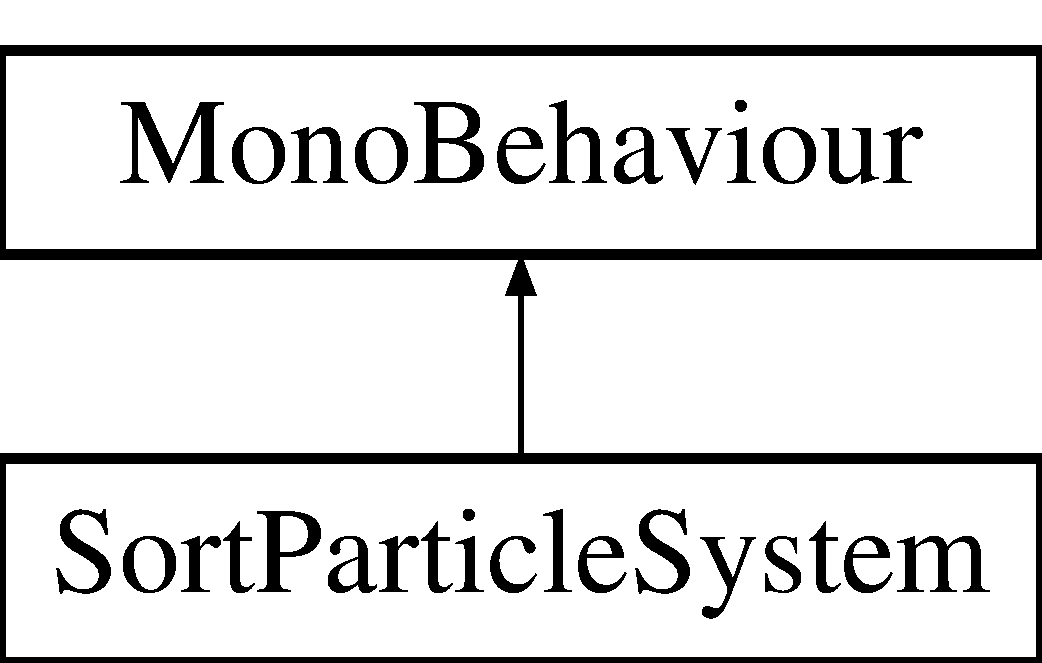
\includegraphics[height=2.000000cm]{class_sort_particle_system}
\end{center}
\end{figure}
\subsection*{Metody publiczne}
\begin{DoxyCompactItemize}
\item 
void {\bf Start} ()
\begin{DoxyCompactList}\small\item\em Domyślnie Particle\+System nie ma opcji ustawiania warstwy, na której ma być wyświetlany. \end{DoxyCompactList}\end{DoxyCompactItemize}
\subsection*{Atrybuty publiczne}
\begin{DoxyCompactItemize}
\item 
string {\bf Layer\+Name} = \char`\"{}Particles\char`\"{}
\begin{DoxyCompactList}\small\item\em Nazwa warstwy \end{DoxyCompactList}\end{DoxyCompactItemize}


\subsection{Opis szczegółowy}
klasa \doxyref{Sort\+Particle\+System}{str.}{class_sort_particle_system} 



\subsection{Dokumentacja funkcji składowych}
\index{Sort\+Particle\+System@{Sort\+Particle\+System}!Start@{Start}}
\index{Start@{Start}!Sort\+Particle\+System@{Sort\+Particle\+System}}
\subsubsection[{Start()}]{\setlength{\rightskip}{0pt plus 5cm}void Sort\+Particle\+System.\+Start (
\begin{DoxyParamCaption}
{}
\end{DoxyParamCaption}
)}\label{class_sort_particle_system_a671745a1f19ee8e655d8cd4ed2ccd06e}


Domyślnie Particle\+System nie ma opcji ustawiania warstwy, na której ma być wyświetlany. 



\subsection{Dokumentacja atrybutów składowych}
\index{Sort\+Particle\+System@{Sort\+Particle\+System}!Layer\+Name@{Layer\+Name}}
\index{Layer\+Name@{Layer\+Name}!Sort\+Particle\+System@{Sort\+Particle\+System}}
\subsubsection[{Layer\+Name}]{\setlength{\rightskip}{0pt plus 5cm}string Sort\+Particle\+System.\+Layer\+Name = \char`\"{}Particles\char`\"{}}\label{class_sort_particle_system_a9d51c7cdcf653de70767eef676bce85d}


Nazwa warstwy 



Dokumentacja dla tej klasy została wygenerowana z pliku\+:\begin{DoxyCompactItemize}
\item 
C\+:/\+Users/\+Paul/\+Projects/\+Unity\+Game/\+Projekt/\+Assets/\+Code/Sort\+Particle\+System.\+cs\end{DoxyCompactItemize}

\section{Dokumentacja klasy Start\+Screen}
\label{class_start_screen}\index{Start\+Screen@{Start\+Screen}}


Klasa umożliwi ewentualne rozpoczęcie gry od ekranu startowego, a nastepnie przeniesienie do pierwszego etapu gry.  


Diagram dziedziczenia dla Start\+Screen\begin{figure}[H]
\begin{center}
\leavevmode
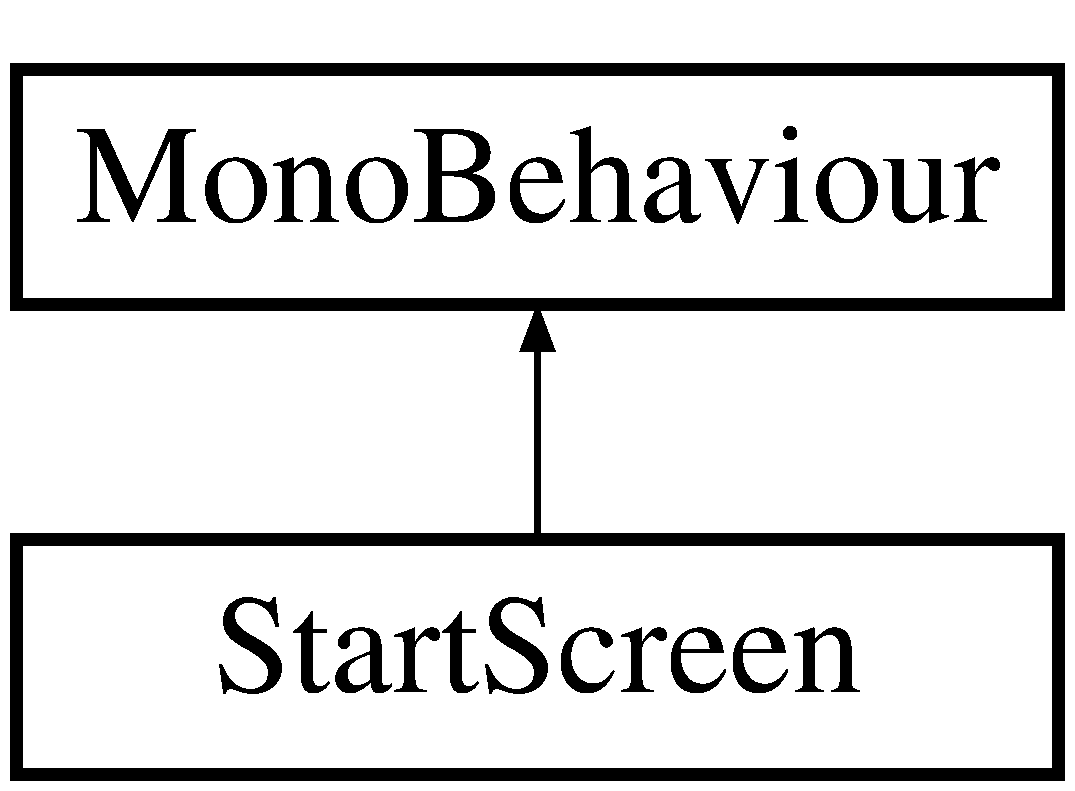
\includegraphics[height=2.000000cm]{class_start_screen}
\end{center}
\end{figure}
\subsection*{Metody publiczne}
\begin{DoxyCompactItemize}
\item 
void {\bfseries Update} ()\label{class_start_screen_ab77f1e4efe3c8c259e8957dccc8ef8ae}

\end{DoxyCompactItemize}
\subsection*{Atrybuty publiczne}
\begin{DoxyCompactItemize}
\item 
string {\bfseries First\+Level}\label{class_start_screen_a0dc7263b0b6fa4ccab70f1ebab366ade}

\end{DoxyCompactItemize}


\subsection{Opis szczegółowy}
Klasa umożliwi ewentualne rozpoczęcie gry od ekranu startowego, a nastepnie przeniesienie do pierwszego etapu gry. 



Dokumentacja dla tej klasy została wygenerowana z pliku\+:\begin{DoxyCompactItemize}
\item 
C\+:/\+Users/\+Paul/\+Projects/\+Unity\+Game/\+Projekt/\+Assets/\+Code/Start\+Screen.\+cs\end{DoxyCompactItemize}

%--- End generated contents ---

% Index
\backmatter
\newpage
\phantomsection
\clearemptydoublepage
\addcontentsline{toc}{chapter}{Indeks}
\printindex

\end{document}
